\chapter{Interweave System}
\label{chap:IS}
\index{Interweave system|(}
%}\vspace{0.4cm}
Secondary access to the licensed spectrum is viable only if the interference is avoided at the primary system. %In this regard, different paradigms have been conceptualized in the existing literature. 
Among the different paradigms conceptualized in the literature, ISs have been extensively investigated. %This makes performance characterization of a cognitive radio system critical, hence, an interesting research problem. 
In order to enable interference-free access to the licensed spectrum, ISs employ spectrum sensing at the Secondary Transmitter (ST). 
Spectrum sensing (or only sensing) is necessary for detecting the presence or the absence of a PU signal. In this way, sensing assists the ISs in protecting the PRs against harmful interference. \tc{A sensing mechanism} at the ST can be accomplished by listening to the signal transmitted by the PT.
The existing models (termed as baseline models), investigated in the literature \cite{Liang08, Sharma14, Pradhan15}, characterize the performance of IS in terms of a sensing-throughput tradeoff. However, this characterization assumes the perfect knowledge of the involved channels at the ST, which is unavailable in practice. 
%Baseline models investigated in the literature characterize the performance of IS in terms of a sensing-throughput tradeoff, however, this characterization assumes the perfect knowledge of the involved channels at the secondary transmitter, which is unavailable in practice. %As a result, these models depict an ideal scenario, thereby making the performance characterization based on these models disputable and impractical for hardware deployment. 
Motivated by this fact, this chapter, which is based on \citeK{Kaushik15_CC, Kaushik16_TWC, Kaushik16_VTC1}, proposes a novel approach to incorporate channel estimation corresponding to the IS in the system model, %, whereby imposes a fundamental limit on the performance of cognitive radio as interweave system. 
%In order to enable secondary access to the licensed spectrum, several paradigms have been conceptualized. Of these, interweave systems that employ spectrum sensing have been widely investigated in the literature. According to which, the interference is avoided by sustaining detection probability above a desired level. Upon satisfying the constraint, the secondary transmitter intends to optimize its throughput. 
%In literature, this optimization has been characterized in terms of sensing-throughput tradeoff. 
%Conventional investigations on the performance of interweave system that employ spectrum sensing at the secondary transmitter have assumed the perfect knowledge of interacting channels. 
%Sensing the energy over the primary user spectrum has been widely investigated in the literature. 
%According to which, an optimum throughput can be achieved by operating at a suitable sensing time. 
%This characterization however considers the knowledge of the channels at the secondary transmitter, this, depicts an ideal scenario. %(primary transmitter - secondary transmitter, secondary transmitter - secondary receiver, primary transmitter - secondary receiver)
%While considering a hardware deployment, this knowledge is essential. Motivated by this fact, we propose a novel system model that incorporates channel estimation. 
 and consequently investigates the impact of imperfect channel knowledge on the performance of the IS. 

More particularly, the variations induced in the detection probability affect the detector's performance at the ST. Since the detector installed at the ST is largely responsible for regulating the interference, uncertainty in its performance may result in severe interference at the PRs. In order to capture this uncertainty, an average constraint and an outage constraint\footnote{The outage constraint is an essential metric employed for designing communication systems, which ensures that the outage occurs no more than a certain percentage of time.} on the detection probability are proposed.
%Using these constraints, we characterize the true performance of the IS. 
%Our analysis reveals that the ideal scenario considerably overestimates the performance of the IS. 
The analysis, performed in this chapter, reveals that an appropriate choice of the estimation time and the sensing time intervals\footnote{Throughout the thesis, the estimation time interval and sensing time interval are used interchangeably with estimation time and sensing time, respectively.} can effectively control the performance degradation. Thus, depicting the achievable secondary throughput of the IS.

%%%%%%%%%%%%%%%%%%%%%%%%%%%%%%%%%%%%%%%%%%%%%%%%%%%%%%%%%%%%%%%%%%%%%%%%%%%%%%%%%%%%%%%%%
%\section{Introduction}
%%%%%%%%%%%%%%%%%%%%%%%%%%%%%%%%%%%%%%%%%%%%%%%%%%%%%%%%%%%%%%%%%%%%%%%%%%%%%%%%%%%%%%%%%
%\subsection{Background}
%Goldsmith \textit{et .al} \cite{Goldsmith09}

\section{Related Work}


%In this regard, a novel approach that incorporates channel estimation in the system model is established, and consequently the impact of imperfect channel knowledge on the performance of the IS is investigated. More particularly, the variation induced in the detection probability affects the detector's performance at the secondary transmitter, which may result in severe interference at the PRs. In order to control the excessive interference, average and outage constraints on the detection probability are proposed. 

For detecting a PU signal, several techniques such as\index{Spectrum sensing!energy detection} energy-based detection (or energy detection), matched filtering-based, cyclostationary-based and feature-based detection exist \cite{Sharma15, Axell12}. Because of its versatility towards unknown PU signals and its low computational complexity, energy detection has been extensively investigated in the literature \cite{Urkowitz, Kostylev02, Alouini03, Herath09, Mariani10}. In this technique, the decision is accomplished by comparing the power received at the ST to a decision threshold. In reality, the ST encounters variations in the received power due to the existence of thermal noise at the receiver and fading in the channel. Subsequently, these variations lead to sensing errors described as misdetection and false alarm, %The characterization of sensing errors as detection probability and false alarm probability has been studied in \cite{tan08}. 
which limit the performance of the IS. In order to determine the performance of a detector, it is essential to obtain the expressions of detection probability and false alarm probability.

In particular, detection probability is critical for IS because it protects the PR from the interference induced by the ST. As a result, the ISs have to ensure that they operate above a target detection probability \cite{peh07}. Therefore, the characterization of the detection probability becomes absolutely necessary for the performance analysis of the IS. In this context, Urkowitz \cite{Urkowitz} introduced a probabilistic framework for characterizing the sensing errors, however, the characterization accounts only for the noise in the system. 

To encounter the variation caused by channel fading, a frame structure has been introduced in \cite{Liang08}, \tc{assuming that the channel remains} constant over the frame duration (corresponds to a quasi-static block fading). Upon exceeding the frame duration, the system may observe a different realization of the channel. Based on this frame structure, the performance of the IS has been investigated in terms of a deterministic (corresponding to a non-random behaviour) channel \cite{Liang08, Sharma14, Pradhan15} \index{Channel!determistic channel} and a random channel\index{Channel!random channel} \cite{Kostylev02, Alouini03, Herath09}. \tc{In the thesis, the deterministic channel symbolizes that the performance of the CR system is analyzed for a specific frame, i.e., for a particular realization of the channel. Whereas the random channel represents that the performance is evaluated over multiple frames, i.e., the CR system observes multiple realizations of the channel. For the latter case, a fading model is employed to capture the random behaviour of the channel.} 
%Complementing the analysis in \cite{Liang08, Sharma14, Pradhan15}, the involved channels are considered to be deterministic and random.} 

%The long-term characterization is a classical approach that applies a fading model to average out the variation in the received power. Subject to the deployment scenarios\footnote{These scenarios include urban, suburban and rural, or indoor and outdoor from a different perspective.}, different fading models -- Rice, Rayleigh, Nakagami-$m$ and Log-normal can be employed \cite{Simon00}. The analytical expressions for the expected detection probability for these fading models are characterized in \cite{Kostylev02, Alouini03, Herath09}. Considering a CR system, this approach has some major drawbacks. Fading models depict a long-term characterization of the system, however, short-term or bursty interference that may lead to outage is ignored, thereby deteriorating the performance of a primary system. Moreover, fading models are specific to the deployment scenario, hence, knowledge of the fading model is necessary when designing a CR system. Apart from that, every fading model contains certain model parameters. As a result, estimation of these parameters at the ST \cite{Kaushik14}, particularly during the initial phase of the deployment, imposes an additional overhead on the secondary system. In practice, due to mobility, most systems are likely to violate stationarity over a long duration. Thus, it becomes challenging to track these model parameters. As a consequence, these drawbacks restrict the applicability of this approach to practical CR systems. 

%To overcome the aforementioned drawbacks, an alternative approach that considers the short-term characterization has been established \cite{Liang08, Sharma14, Pradhan15} in such a way that the performance can be analyzed for a single frame\footnote{By a single frame, we refer to the statistical realizations of the received power, whereas \cite{Liang08, Sharma14, Pradhan15} consider the temporal realizations of the same across several frames. Considering ergodic behaviour of the noise, the performance characterization under these two scenarios are equivalent.}. In this way, unlike long-term approach, we preclude the variation due to the channel and consider the variation due to noise in the system. Subsequently, this approach does not need to consider the deployment of the fading model and its complexities thereafter. Motivated by these facts, we focus on the short-term approach for performance analysis.  


Besides the detection probability, false alarm probability has a large influence on the throughput achieved by the secondary system. %Further, the characterization of the false alarm probability requires the knowledge of the noise power. Subject to a given uncertainty \cite{Tan08}, this knowledge can be acquired through hardware calibration. 
%\subsection{Problem Formulation}
Recently, the performance characterization of CR systems in terms of a sensing-throughput tradeoff\index{Tradeoffs!sensing-throughput tradeoff} has received significant attention \cite{Liang08, Juarez11, Sharkasi12, Pradhan15}. According to Liang \textit{et al.} \cite{Liang08}, the ST assures a reliable detection of a PU signal by retaining the detection probability above a desired level with an objective of maximizing the throughput at the SR. In this way, the sensing-throughput tradeoff depicts a suitable sensing time interval that achieves a maximum secondary throughput. To characterize the detection probability and the secondary throughput, the system requires the knowledge of interacting channels, namely, a \textit{sensing} channel, an \textit{access} channel and an \textit{interference} channel, \tc{refer to} \figurename~\ref{fig_IS:scenario}\footnote{As the interference to the PR is controlled by a regulatory constraint over the detection probability, in this view, the interaction with the PR is excluded in the considered scenario \cite{Liang08}.}. The baseline models, investigated in the literature, assume the knowledge of these channels to be available at the ST. 
However, in practice, this knowledge is not available and, thus, it needs to be estimated by the secondary system. As a result, the existing solutions for the IS are considered inadequate from a practical viewpoint. 


%\tc{Following the previous discussion, it is apparent that the knowledge of the sensing, interference and access channels is crucial for characterizing the detection probability and the secondary throughput. 
%In practice, the knowledge about the involved channels can be estimated either (i) directly by using the conventional channel estimation techniques such as training sequence based \cite{Stoica03} and pilot-based \cite{Gifford05, Gifford08} channel estimation or (ii) indirectly by estimating the received signal to noise ratio \cite{Chav11, Sharma13}. Such techniques are well-known for delivering accuracy channel estimates, hence, mostly employed for the channel estimation in state-of-the-art wireless standards. Despite this, they (i) increase the complexity of the channel estimation in terms of the mathematical operations and (or) on demand a demodulation of the PU signal at the ST. 
As a matter of fact, the sensing and the interference channels related to the CR system (refer to \figurename~\ref{fig_IS:scenario}) represent the channels between two different (primary and secondary) systems. In this context, it becomes challenging to select the estimation methods in such a way that low complexity and versatility (towards different PU signals) requirements are satisfied. These issues, discussed later in Section \ref{ssec_IS:pa}, render the existing estimation techniques \cite{Stoica03, Gifford05, Gifford08, Chav11, Sharma13} unsuitable for hardware implementations. 
%Existing works assume it to be known at the ST. In reality, due to  this knowledge is not available at the ST. 
%The channel, regarded as deterministic and unknown, is expected to remain constant over a frame duration, 
To tackle the issue related to the channel estimation, a received power-based estimation at the ST and at the SR for the sensing and the interference channels is employed, respectively.
Considering the fact that the access channel corresponds to the link between the ST and the SR, conventional channel estimation techniques such as pilot-based channel estimation at the ST is employed.

\tc{  
Inherent to the estimation process, the variations due the channel estimation translate to the variations in the performance parameters, namely detection probability and secondary throughput. In particular, the variations induced in the detection probability cause uncertain interference at the PR, which may severely degrade the performance of a CR system. The detrimental effect due to the time allocation for the channel estimation and the uncertain interference due to imperfect channel knowledge have not been considered in \cite{Liang08, Juarez11, Sharkasi12, Pradhan15} or studied partially in \cite{Chav11, Cao14}. In this context, the performance characterization of an IS with imperfect channel knowledge remains an open problem. %As a result, we apply received power estimation that entails the knowledge of the channel for the sensing channel, \tc{refer} \figurename~\ref{fig_IS:scenario}. 
%Upon sustaining the detection probability at a desired level, the ST aims to optimize its throughput. This phenomenon is characterized as a sensing-throughput tradeoff by Liang \textit{et al.} \cite{Liang08}. At the ST, the sensing-throughput tradeoff renders a suitable sensing time that achieves an optimum throughput for a given received power. Several contributions \cite{Liang08, Juarez11, Sharkasi12, Pradhan15} have considered this tradeoff to characterize the performance of the IS. These contributions investigated in the literature assume the knowledge of the interacting channels at the ST, which include an access channel from the ST and an interference channel from PT to the SR, \tc{refer} \figurename~\ref{fig_IS:scenario}. Hence, are considered idealistic and implausible for deployment. 
%The knowledge of these channels is not available in reality, thus, needs to be estimated by the SR and made available to the ST through a feedback channel. Moreover, due to the presence of noise in the system, this knowledge is never perfect. 
%Considering a hardware deployment, it is important to determine the performance of the IS based on channel estimation. %A similar analysis is performed in \cite{Kaushik15}, where the authors employ the received power estimation to control transmit power at the ST deployed as an underlay system. However, in this paper, we intend to capture the effect of estimation on the performance of an IS. %Furthermore, the effect of received power estimation on the performance of the system is an open problem.
%Moreover, the knowledge of the channels are not directly available. 
%The knowledge for the channel  For the channel (PT-SR), the channel knowledge is not directly available  
%In parallel to that, the variations in the further translates to the variation in the secondary system's throughput. Moreover, the estimation of the access and the interference channels imposes an additional variation on the throughput. 
Motivated by this fact, this chapter focuses on the performance characterization of the IS in terms of sensing-throughput tradeoff taking these aforementioned aspects into account.}

%Recently, sensing throughput tradeoff has been considered as an important metric to evaluate the performance of the IS. However, the influence of received power estimation on the performance of the system is an open research problem. %Hence, we tend to include the receiver power estimation.  
%With the inclusion of estimation error, the IS intends to operate at an suitable estimation time such that a maximum distortion remains below a desired level. 
%For a fixed the detection probability, the threshold and sensing time are determined. %Apart from these, the characterization of the false alarm probability requires the perfect knowledge of noise power at the ST. Considering a practical scenario, this is a rarely the situation. Hence, it is important to include the effect of noise uncertainty on the performance of the system. 
\section{Contributions}
The major contributions of this chapter can be summarized as follows:
%\begin{itemize}
\subsection{\tc{Analytical Framework}}
%\item 
In contrast to the existing models that assume perfect knowledge of the channels, the main goal of this chapter is to derive an analytical framework that constitutes the estimation of: (i) sensing channel at the ST, (ii) access channel and (iii) interference channel at the SR. As illustrated later in \figurename~\ref{fig_IS:fs}, under this framework, a novel integration of the channel estimation in the secondary system's frame structure is proposed. According to which the samples considered for channel estimation (of the sensing channel) are accounted also for the sensing such that the time resources within the frame are utilized efficiently. Furthermore, the estimation techniques are selected in such a way that the hardware complexity and the versatility towards unknown PU signals requirements (as considered while employing an energy based detection) are not compromised. In this context, a received power-based estimation for the sensing and the interference channels is proposed. Based on proposed framework, this chapter characterizes the performance of the IS by considering the performance degradation due to: \begin{itemize} \item the variations caused by imperfect channel knowledge and \item the inclusion of time allocated for performing channel estimation. \end{itemize} 
The proposed analytical framework is further complemented by considering a random behaviour of the interacting channels (or channel fading). Based on the derived expressions, the performance of the IS that employs channel estimation is evaluated, where the interacting channels are subjected to Nakagami-$m$ fading\index{Nakagami-$m$ fading}.


%\item
\subsection{\tc{Imperfect Channel Knowledge}}
In order to capture the variations induced due to imperfect channel knowledge, the cumulative distribution functions (cdfs) of performance parameters such as detection probability and achievable secondary throughput are characterized. More importantly, the cdf of the detection probability is utilized to incorporate two PU constraints, namely, an average constraint\index{Interference constraint!average constraint} and an outage constraint\index{Interference constraint!outage constraint} on the detection probability. In this way, the proposed approach is able to control the amount of uncertainty in the interference caused at the PR due to the imperfect channel knowledge. 
%\item 
\subsection{\tc{Estimation-Sensing-Throughput Tradeoff}\index{Tradeoffs!estimation-sensing-throughput tradeoff}}
Subject to the average and the outage constraints, the expressions of the sensing-throughput tradeoff that capture the aforementioned variations and evaluate the performance loss (in terms of the achievable secondary throughput) are established. In particular, two different optimization approaches for countering the variations in the IS and determining suitable estimation and suitable sensing time intervals, which attain a maximum secondary throughput, are proposed. Finally, a fundamental tradeoff between estimation time, sensing time and achievable secondary throughput is depicted. This tradeoff is exploited to determine suitable estimation and suitable sensing time intervals that depict the maximum achievable performance of the IS. 
%\subsection{\tc{Channel fading}}
Besides, %the variations due to the channel estimation and the channel fading are jointly captured by means of an outage constraint on the detection probability. %Subsequently, an expression of the sensing-throughput tradeoff subject to the aforementioned constraint is obtained.
%In addition, an estimation-sensing-throughput tradeoff is established for the random scenario. 
%In this regard, 
the estimation-sensing-throughput tradeoff is adapted to the scenarios with channel fading, thus determining the achievable secondary throughput subject to the random behaviour of the channels.
 
%\end{itemize}

%\subsection{Organization}
%The subsequent sections of the paper are organized as follows: Section \ref{sec_IS:sys_mod} describes the system model that includes the deployment scenario and the signal model. \tc{Section \ref{sec_IS:pr_mod} presents the problem description and the proposed approach.} Section \ref{sec_IS:ana} characterizes the distribution functions of the performance parameters and establishes the sensing-throughput tradeoff subject to average and outage constraints. Section \ref{sec_IS:num_ana} analyzes the numerical results based on the obtained expressions. Finally, Section \ref{sec_IS:conc} concludes the paper. Table \ref{tb_IS:tb1} lists the definitions ef acronyms and important mathematical notations used throughput the paper.

%\begin{table}
%%\vspace{-0.4cm}
%\renewcommand{\arraystretch}{1.4}
%\caption{Definitions of Acronyms and Notations used}
%%\vspace{-0.6cm}
%\label{tb_IS:tb1}
%\centering
%\scriptsize{
%%\begin{tabular}{l||l}
%\begin{tabular}{p{0.25\columnwidth}||p{0.6\columnwidth}}
%\hline
%\bfseries Acronyms and Notations & \bfseries Definitions \\
%\hline\hline
%AC, OC & average constraint, outage constraint \\ \hline
%%AWGN & Additive White Gaussian Noise  \\ \hline
%CR & cognitive radio\\ \hline
%CSC, CSC-BS, MC-BS, MS & cognitive small cell, cognitive small cell-base station, macro cell-base station, mobile station\\ \hline
%IM, EM & ideal model, estimation model \\ \hline
%IS & interweave system \\ \hline
%PU - PT, PR & primary user - primary transmitter, primary receiver \\ \hline
%SU - ST, SR & secondary user - secondary transmitter, secondary receiver \\ \hline
%$\mathcal H_1, \mathcal H_0$ & Signal plus noise hypothesis, noise only hypothesis\\ \hline
%$\fsam$ & Sampling frequency\\ \hline
%$\test, \tsen$ & Estimation time, sensing time interval\\ \hline
%$T$ & Frame duration\\ \hline
%$\pd, \pfa$ & Detection probability, false alarm probability \\ \hline
%$\pdd$ & Target detection probability\\ \hline
%$\mpd$ & Outage constraint over detection probability\\ \hline
%$\hpo, \hpt, \hs$ & Channel coefficient for the link PT-ST, PT-SR, ST-SR \\ \hline
%$\snrrcvd, \snrso$ & Signal to noise ratio for the link PT-ST, ST-SR \\ \hline
%$\snrpt$ & Interference (from PT) to noise ratio for the link PT-SR \\ \hline
%$\rs$ & Throughput at SR\\ \hline
%$\cz,\co$ & Date rate at SR without and with interference from PT  \\ \hline
%$\mu$ & Threshold for the energy detector\\ \hline
%$F_{(\cdot)}$ & Cumulative distribution function of random variable $(\cdot)$\\ \hline
%$f_{(\cdot)}$ & Probability density function of random variable $(\cdot)$\\ \hline
%$\hat{(\cdot)}$ & Estimated value of ($\cdot$)\\ \hline
%$\tilde{(\cdot)}$ & Suitable value of the parameter ($\cdot$) that achieves maximum performance \\ \hline
%$\mathbb E_{(\cdot)}$ & Expectation with respect to ($\cdot$) \\ \hline
%$\p$ & Probability measure \\ \hline
%\textbf{T}$(\cdot)$ & Test statistics\\ \hline
%%$x_{(\cdot)}[n], y_{(\cdot)}[n]$ & $n\supe{th}$ sample of the transmitted discrete and real signal, received discrete and real signal at ($\cdot$) \\ \hline
%%$P\sub{Tx, $(\cdot)$},  P\sub{Rx, $(\cdot)$}$ & Power transmitted, power received at ($\cdot$) \\ \hline
%$\spo,  \npo$ & Signal variance at PT, noise variance at ST and SR\\ \hline
%%$\Gamma(\cdot)$ & Gamma function\\ \hline
%%$\Gamma(\cdot, \cdot)$ & Regularized incomplete upper Gamma function\\ \hline
%%$\Gamma^{-1}(\cdot, \cdot)$ & Inverse of regularized incomplete upper Gamma function\\ \hline
%%$\mathcal N, \cchi2, \ncchi2$ & Normal, central chi-squared, non-central chi-squared distribution\\ \hline
%$ \Ks$ & Number of pilot symbols used for pilot based estimation at the SR for $\hs$ \\ \hline
%$ \Kp$ & Number of samples used for received power based estimation at the SR for $\hpt$ \\ \hline
%%$\as, \bs, \ap, \bp$ & Model parameters of Gamma distribution \\ \hline
%%$\ls$ & Non-centrality parameter of  $\ncchi2$ distribution \\ \hline
%\end{tabular}}
%\end{table}
% 
%%%%%%%%%%%%%%%%%%%%%%%%%%%%%%%%%%%%%%%%%%%%%%%%%%%%%%%%%%%%%%%%%%%%%%%%%%%%%%%%%%%%%%%%%
\section{System Model} \label{sec_IS:sys_mod}
%%%%%%%%%%%%%%%%%%%%%%%%%%%%%%%%%%%%%%%%%%%%%%%%%%%%%%%%%%%%%%%%%%%%%%%%%%%%%%%%%%%%%%%%%
\subsection{Interweave Scenario}

\begin{figure}[!ht]
\centering
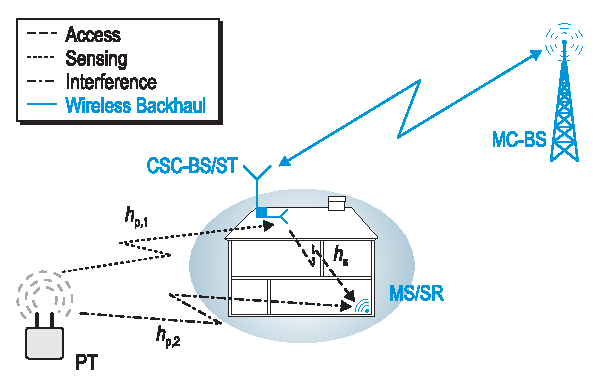
\includegraphics[width = \figscale]{figures/CR_Scenario_Interweave}
\caption{A cognitive small cell scenario demonstrating: (i) the interweave paradigm, (ii) the associated network elements, which constitute cognitive small cell-base station/secondary transmitter (CSC-BS/ST), mobile station/secondary receiver (MS/SR), macro cell-base station (MC-BS) and primary transmitter (PT), (iii) the interacting channels: sensing ($\hpo$), access ($\hs$) and interference ($\hpt$).} 
\label{fig_IS:scenario}
%\vspace{-0.3cm}
\end{figure}
%In order to consider the deployment of the IS, the CSC, a CR application that characterizes a small cell deployment that fulfills the spectral requirements for mobile stations (MSs) operating indoor, \tc{refer to} \figurename~\ref{fig_IS:scenario} is considered. For the disposition of the CSC in the network, the following key elements are essential: a CSC-base station (CSC-BS), a macro cell-base station (MC-BS) and MS, refer to \figurename~\ref{fig_IS:scenario}. MSs are the indoor devices served by the CSC-BS over an access channel ($\hs$). Furthermore, the MC-BS is connected to several CSC-BSs over a wireless backhaul\footnote{A wireless backhaul is a point-to-point wireless link between the CSC-BS and MC-BS that relays the traffic generated from the CSC to the core network.}. Moreover, the transmissions from the PT can be listened by the CSC-BS and the MS over sensing ($\hpo$) and interference channel ($\hpt$), respectively. %Although the MC-BS and the MS already exist in the conventional cellular architecture, to incorporate the opportunistic access inside the CSC, it is necessary to consider a functionality upgrade. 
To consider the applicability of IS, the CSC, a CR application illustrated in the previous chapter, is transformed into an interweave scenario. Considering the fact that the IS is employed at the CSC-BS, the CSC-BS and the MS represent the ST and the SR, respectively. A hardware prototype of the CSC-BS operating as IS was presented in \cite{Kaushik13}. For simplification, a PU constraint based on false alarm probability was considered in \cite{Kaushik13}. With the purpose of improving system's reliability, the analysis is extended to employ a PU constraint on the detection probability. 

\tc{Complementing the analysis depicted in \cite{Liang08},} a slotted medium access for the IS is considered, where the time axis is segmented into frames of length $T$, according to which the ST employs periodic sensing. Hence, each frame consists of a sensing slot $\tsen$ and the remaining duration $T - \tsen$ is utilized for data transmission. For small $T$ relative to the PUs' expected ON/OFF period, the requirement of the ST to be in alignment to PUs' medium access can be relaxed \cite{Wang09, Tang11, Zhao12}.  
 
\subsection{Signal Model}
%According to interweave system, ST considers a hypothesis testing to determine the presence ($\mathcal{H}_1$) or absence $(\mathcal{H}_0)$ of a signal transmitted by the PR. 
Subject to the underlying hypothesis that illustrates the presence $(\mathcal{H}_1)$ or the absence ($\mathcal{H}_0$) of a PU signal, the discrete and complex signal received at the ST is given by\index{Spectrum sensing!energy detection}  
\begin{equation}
\yrcvd[n] = 
\begin{cases}
\hpo \cdot \xp[n] + \wst[n] & : \mathcal{H}_1 \\
\wst[n] & :\mathcal{H}_0
\end{cases},
\label{eq_IS:sys_mod_p1s}
\end{equation}
where $\xp[n]$ corresponds to a discrete and complex sample transmitted by the PT, $|\hpo|^2$ represents the power gain of the sensing channel for a given frame and $\wst[n]$ is circularly symmetric Additive White Gaussian Noise (AWGN) $\mathcal{CN}(0, \npo)$ at the ST. 

\tc{According to \cite{Liang08}, the signal $\xp[n]$ transmitted by the PUs} can be modeled as: (i) a phase shift keying modulated signal, or (ii) a Gaussian signal. The signals that are prone to high inter-symbol interference or entail precoding, for instance Orthogonal Frequency Division Multiplexing (OFDM)\index{OFDM} signal with linear precoding, can be modeled as Gaussian signals. In this chapter and the Chapter \ref{chap:HS} (dedicated to the HS), the analysis is focused on the latter case, i.e., the primary and the secondary systems employ OFDM to carry out their transmission. In contrast, Chapter \ref{chap:US} associated with the US, considers the former case for the analysis. As a result, the mean and the variance for the signal and the noise are determined as $\e{}{\xp[n]} = 0$, $\e{}{\wst[n]} = 0$, $\e{}{|\xp[n]|^2} = \spo$ ($= \ptranpt$) and $\e{}{|\wst[n]|^2} = \npo$. The channel $\hpo$ is considered to be independent of $\xp[n]$ and $\wst[n]$. Thus, $\yrcvd[n]$ is also an independent and identically distributed (i.i.d.) random process. %The true received power is defined as
%\begin{align}
%\bprcvd = \e{}{|\yrcvd|^2}.
%\label{eq_IS:tprcvd}
%\end{align}
%Based on (\ref{eq_IS:tprcvd}), the received SNR at the ST is $\snrrcvd = \frac{\bprcvd}{\npo} - 1$.

Similar to (\ref{eq_IS:sys_mod_p1s}), during data transmission, the discrete and complex received signal at the SR conditioned on the detection probability ($\pd$) and the false alarm probability ($\pfa$) is given by
\begin{equation}
\ys[n] = 
\begin{cases}
\hs \cdot \xs[n] + \hpt \cdot \xp[n] +  \wsr[n] & : 1 - \pd \\
\hs \cdot \xs[n] + \wsr[n] & : 1 - \pfa
\end{cases},
\label{eq_IS:sys_mod_ss}
\end{equation}
%and on the other side, the interference signal at the SR, transmitted by the PR follows 
%\begin{equation}
%\yp[n] = \sqrt{\gpt \cdot \apt}/ \cdot \xp[n] + w[n],
%\label{eq_IS:sys_mod_p2s}
%\end{equation}
where $\xs[n]$ corresponds to discrete and complex sample transmitted by the ST and $\wsr[n]$ is the AWGN \index{AWGN} at the SR with $\mathcal{CN}(0, \npo)$\footnote{In practice, the noise power at different network nodes (the ST, the SR and the PR) have different values. The fact is, only the signal to noise ratios  received at these nodes are affected due to these different values, which are already included in the performance analysis. For the brevity of the exposition, in the thesis, the noise powers at these nodes are expressed using a single notation ($\npo$).}. Further, $|\hs|^2$ and $|\hpt|^2$ represent the power gains for the access and the interference channels, \tc{refer to} \figurename~\ref{fig_IS:scenario}. 
%The %received powers at the SR from ST and PR are evaluated as $\ps = \s{\test \fsam}{|\ys[n]^2|}$ and $\pp = \s{\test \fsam}{|\yp[n]^2|}$ %Likewise (\ref{eq_IS:sys_mod_p1s}), $\nap[n]$ and $\nas[n]$ represents circularly symmetric AWGN at PR and ST with zero mean and variance $\e{}{|\nap[n]|^2} = \npp$ and $\e{}{|\nas[n]|^2} = \nps$ correspondingly. Consider that $\ps$, $\ps$ and $\pp$ correspond to power for a given frame. 
%\subsubsection{Channel}
%, where $\bpp = \e{}{\pp}$ and $\bps = \e{}{\ps}$ correspond to their true value. Similar to ST-PR, the 
%received SNRs over the links ST-SR and PT-ST are $\snrs = \frac{\e{}{|\sqrt{\hs} \cdot \xs[n]|^2}}{ \npo}$ and $\snrp = \frac{\e{}{|\sqrt{\hpt} \cdot \xp[n]|^2}}{\npo}$.


%\section{\tc{Problem Description and Proposed Approach}} \label{sec_IS:pr_mod}
\subsection{\tc{Problem Description}}\label{ssec_IS:pd}
%\subsection{Sensing}
\tc{In accordance with the conventional frame structure}, the ST performs sensing for a duration of $\tsen$. The test statistics\index{Test statistics} $\ts$ at the ST is evaluated as   
\begin{align}
\ts = \s{\tsen \fsam}{ |\yrcvd[n]|^2} \mathop{\gtrless}_{\mathcal{H}_0}^{\mathcal{H}_1} \mu, 
\label{eq_IS:test_st}
\end{align}
where $\mu$ is the decision threshold, $\fsam$ represents the sampling frequency and $\textbf{y}$ is a vector with $\tsen \fsam$ samples. $\ts$ represents a random variable, whereby the characterization of the cdf depends on the underlying hypothesis. With regard to the Gaussian signal model, which corresponds to the OFDM signal transmitted by the PU, $\ts$ follows a central chi-squared\footnote{It is worthy to mention here that, by avoiding the Gaussian approximation that exists due to the application of central limit theorem\index{Central limit theorem}, thereby limiting the applicability of the considered analysis to only large sample sizes. In the thesis, an effort has been made to derive the theoretical expressions so that the performance analysis is valid for all sample sizes.}  ($\cchi2$) distribution for both hypotheses $\mathcal{H}_0$ and $\mathcal{H}_1$ \cite{Kay}. 
%\begin{equation}
%\ts = 
%\begin{cases}
%\sim \ncchi2  : \mathcal{H}_1 \\
%\sim \cchi2  : \mathcal{H}_0 \\
%\end{cases},
%\label{eq_IS:sys_mod_ss}
%\end{equation}
%Considering large number of samples $\fsam \tsen$ are used to evaluate $\ts$. It is possible to apply Central Limit Problem to approximate the distribution functions of the mentioned hypotheses as Gaussian distribution. 

As a result, the detection probability\index{Spectrum sensing!detection probability} $(\pd)$ and the false alarm probability\index{Spectrum sensing!false alarm probability} $(\pfa)$ corresponding to (\ref{eq_IS:test_st}) are determined as \cite{Tan08}
\begin{align}
%\pd(\mu, \tsen, \prcvd) &= \mathcal{Q}\left( \frac{\mu - \prcvd}{ \sqrt{\frac{2}{\tsen \fsam}} \prcvd} \right),  \label{eq_IS:pd} 
\pd &= \Gamma\left( \frac{\tsen \fsam}{2}, \frac{\tsen \fsam \mu}{2 \prcvdstpt} \right),  \label{eq_IS:pd} 
\end{align}
\begin{align}
\pfa &= \Gamma\left( \frac{\tsen \fsam}{2}, \frac{\tsen \fsam \mu}{2 \npo} \right),  \label{eq_IS:pfa} 
%\pfa(\mu, \tsen) &= \mathcal{Q}\left( \frac{\mu - \npo}{ \sqrt{\frac{2}{\tsen \fsam}} \npo} \right), \label{eq_IS:pfa}
\end{align}
where $\prcvdstpt$ is the power received over the sensing channel and $\Gamma(\cdot, \cdot)$ represents a regularized upper-incomplete Gamma function \cite{grad}.% and $\bprcvd$ signifies the true received power defined as
%\begin{align}
%\bprcvd = \e{}{|\yrcvd|^2}.
%\label{eq_IS:tprcvd}
%\end{align}
 %Due to the presence of the estimation received power $\prcvd$ in (\ref{eq_IS:pd}), $\pd$ corresponds to a random variable.

%The detection probability of the primary signal and the throughput achieved at the SR depict the performance of the IS. 

%\subsection{Sensing-Throughput tradeoff}
Following the characterization of $\pfa$ and $\pd$, Liang \textit{et al.} \cite{Liang08} established a tradeoff between the sensing time and the secondary throughput $(\rs)$ subject to a target detection probability $(\pdd)$. This tradeoff\index{Tradeoffs!sensing-throughput tradeoff} is represented as  
\begin{align}
\trs(\ttsen) &= \maxi_{\tsen} \rs(\tsen) \nonumber \\&= \frac{T- \tsen}{T} \bigg[ \cz (1 - \pfa) \phz +  \co (1 - \pd) \pho  \bigg], \label{eq_IS:thr_id} \\
\text{s.t.} & \text{ } \pd \ge \pdd, \label{eq_IS:thr_id_con} \\ 
\text{where } \cz &= \log_2 \left(1 + |\hs|^2 \frac{\ptranst}{\npo}\right) = \log_2 \left( 1 + \snrso \right) \label{eq_IS:Cap0},\\ 
\co &= \log_2 \left(1 + \frac{|\hs|^2 \ptranst }{|\hpt|^2 \ptranpt  + \npo} \right) \nonumber \\ \quad &= \log_2 \left(1 + \frac{|\hs|^2 \ptranst }{\prcvdsr} \right) = \log_2 \left(1 + \frac{\snrso}{\snrpt + 1}  \right), \label{eq_IS:Cap1} 
\end{align}
where $\phz$ and $\pho$ are the occurrence probabilities for the respective hypothesis, whereas $\snrrcvd$ and $\snrso$ represent the signal to noise ratio for the links PT-ST and ST-SR, respectively, and $\snrpt$ corresponds to interference (from the PT) to noise ratio for the link PT-SR. Moreover, $\ptranpt$ and $\ptranst$ represent the transmit power at the PT and the ST, whereas $\prcvdsr$ corresponds to the received power (which includes the interference power from the PT and the noise power) at the SR. In addition, $\cz$ and $\co$ represent the data rate\index{Data rate}\footnote{\tc{Please note, the following terms the data rate $\cz$, $\co$ and the throughput $\rs$ have been introduced to make a clear distinction between the instantaneous data rate and its average value over the frame duration. Also, the use of the term ``capacity'' is avoided for representing $\cz$ and $\co$, since it implies the optimization of the mutual information over the cognitive channel.}} without and with the interference from the PT. 

In other words, using (\ref{eq_IS:thr_id}), the ST determines a suitable sensing time $\tsen = \ttsen$, such that the secondary throughput is maximized subject to a target detection probability, \tc{refer to} (\ref{eq_IS:thr_id_con}). From the deployment perspective, the tradeoff depicted above has the following fundamental issues:
\begin{itemize}
\item Without the knowledge of the received power $\prcvdstpt$ over the sensing channel, it is not feasible to characterize $\pd$, refer to (\ref{eq_IS:pd}). This renders the characterization of the secondary throughput (\ref{eq_IS:thr_id}) impossible and the constraint defined in (\ref{eq_IS:thr_id_con}) inappropriate. 
\item Moreover, the knowledge of the interference and the access channels is required at the ST, \tc{refer to} (\ref{eq_IS:Cap0}) and (\ref{eq_IS:Cap1}) for characterizing the throughput in terms of $\cz$ and $\co$ at the SR. 
\end{itemize}
%Hence, At An optimum performance is achieved when the ST operates at the desired level, i.e., $\pd = \pdd$. %Hence, based on the expression in (\ref{eq_IS:pd}) and constraint in (\ref{eq_IS:thr_id}), the threshold is evaluated as
%\begin{align}
%\mu(\pdd, \tsen, \bprcvd) = \left( \mathcal{Q}^{-1} (\pdd) \sqrt{\frac{2}{\tsen \fsam}} + 1 \right) \bprcvd. \label{eq_IS:lambda} 
%\end{align}
Taking these issues into account, it is not feasible to employ the performance analysis depicted by this model \tc{(referred as ideal model\index{Ideal model}, hereafter)} for hardware implementation. In the subsequent section, an analytical framework \tc{(also referred as estimation model)} that addresses the aforementioned issues -- including the estimation of the sensing and the access channels at the ST and the interference at the SR -- is proposed. Based on the proposed approach, the performance of the IS in terms of the sensing-throughput tradeoff is investigated. 

\subsection{\tc{Proposed Approach}} \label{ssec_IS:pa}

\tc{In order to overcome the difficulties discussed in Section \ref{ssec_IS:pd}, the following strategy is proposed.
\begin{enumerate}
\item As a first step, the estimation of the involved channels is considered. In order to characterize the detection probability, a received power-based estimation at the ST for the sensing channel is employed. This is done to ensure that the detection probability remains above a desired level. Further, a pilot-based estimation and a received power-based estimation for the access channel and the interference channel are employed at the ST and the SR, respectively, to characterize the secondary throughput. 
\item Next, the variations due to channel estimation in the estimated parameters, namely, received power (for the sensing and the interference channels) and the power gain (for the access channel) are characterized in terms of their cdfs. 
\item In order to investigate the performance of the IS subject to the channel estimation, these variations in the performance parameters, which include the detection probability and the secondary throughput, are characterized in terms of their cdfs. 
\item Finally, the derived cdfs are utilized to obtain the expressions of sensing-throughput tradeoff. Hence, based on these expressions, the impact of imperfect channel knowledge on the performance of the ISs is qualified, and subsequently the achievable secondary throughput at a suitable sensing time is determined. 
\end{enumerate}
}

Considering the channel estimation, it is well-known that systems with transmitter information (which includes the filter parameters, pilot symbols, modulation type and time-frequency synchronization) at the receiver acquire the channel knowledge by listening to the pilot data sent by the ST \cite{Gans71, Gifford05, Gifford08, Anna05}. Other systems, where the receiver possesses either no access to this information or is limited by hardware complexity, procure channel knowledge indirectly by estimating a different parameter that entails the channel knowledge, for instance, received signal power \citeK{Kaushik15_CC} or received signal to noise ratio \cite{Chav11, Sharma13}. Recently, estimation techniques such as pilot-based estimation \cite{Suraweera10, Kim12} and received power-based estimation \citeK{Kaushik15_ICC} have been applied to obtain channel knowledge for the CR systems. However, the performance analysis has been limited to the underlay systems, where the emphasis has been given on modeling the interference at the PR. 

Since the pilot-based estimation requires the knowledge of the PU signal at the secondary system, the versatility (in terms of PU signals) of the secondary system is compromised. On the other side, for the estimation of the received signal to noise ratio\index{Channel estimation!received signal to noise ratio-based},\index{Channel estimation!eigenvalue-based} Eigenvalue (which involves matrix operations) based approach \cite{Sharma13} or iterative approaches such as expectation-maximization have been proposed \cite{Chav11}. Due to the complicated mathematical operations or the complexity of the iterative algorithms, such approaches tend to increase the hardware complexity of the ISs. In order to resolve these issues, a received power-based estimation\index{Channel estimation!received power-based} for the sensing and the interference channels, and a pilot-based estimation\index{Channel estimation!pilot-based} for the access channel is employed. Similar to the energy based detection, since the received power-based estimation involves simple operations on the obtained samples such as magnitude squared followed by summation, the proposed estimation provides a reasonable tradeoff between complexity and versatility. %Unlike the sensing channel, the access and interference channels have to be estimated at the SR and made available at the ST over a low-rate feedback channel. 
%As a result, by proposing the received power estimation and the pilot based estimation, we the versatility and the low complexity requirements of the CR system, which are absolutely essential from the deployment perspective. 

However, with the inclusion of this channel estimation, the system anticipates a performance loss in terms of: (i) temporal resources (time allocation) used and (ii) variations in the aforementioned performance parameters. A preliminary analysis of this performance loss was carried out in \cite{Kaushik15_CC}, where it was revealed that in low signal to noise ratio regime, imperfect knowledge of received power corresponds to a large variation in the detection probability, causing a severe degradation in the performance. However, this performance degradation was determined by means of lower and upper bounds. In this chapter, a more exact analysis is considered, whereby the variations in detection probability are captured by characterizing its cdf, and subsequently apply new probabilistic constraints on the detection probability, which allow the IS to operate at low signal to noise ratio regime. %These constraints are categorized as average and outage constraints corresponds to an conservative or aggressive approach followed by the SU towards the primary system.   

%Besides that, we include channel estimation at the SR to acquire the knowledge of the access and interference channels. 


\subsubsection{Frame Structure\index{Interweave system!frame structure}}
\begin{figure}[!ht]
\centering
\includegraphics[width = \columnwidth]{figures/Frame_Structure}
\caption{Frame structure of the IS illustrating the time allocation of the channel estimation, sensing and data transmission from the perspective of the ST and the SR.} %The estimation of the sensing ($\hpo$) and the interference channel ($\hptw$) estimation occur at the ST. The estimation of the access channel ($\hs$) happens at the SR. Because of the employment of pilot-based channel estimation, the time resources allocated (number of sample used) for its estimation relatively less as compared to the previous two channels used for the channel estimation, it is not considered in the frame structure.} 
\label{fig_IS:fs}
%\vspace{-0.5cm}
\end{figure}
%The inclusion of estimation of the interacting channels causes variations in the parameters $\pd$, $\cz$ and $\co$. Unless characterized, these variations may seriously degrade the performance of the hardware deployed. In this view, we include the estimation of the interacting channels in the system model, thereby characterizing the variations in $\pd$, $\cz$ and $\co$ by means of their their distribution functions $\fpd$, $\fcz$ and $\fco$. By utilizing these expressions, we finally obtain a characterization of sensing-throughput tradeoff. %that depicts an deployment scenario. 
In order to include channel estimation, a frame structure that constitutes estimation $\test$, sensing $\tsen$ and data transmission $T - \tsen$ is proposed, where $\test$ and $\tsen$ correspond to time intervals and \tc{$0 < \test \le \tsen < T$, refer to} \figurename~{\ref{fig_IS:fs}}. Since the estimated values of the interacting channels are required for determining the suitable sensing time (the duration of the sensing phase), the sequence depicted in \figurename~{\ref{fig_IS:fs}} is reasonable for the hardware deployment, whereby estimation is followed by sensing. 
\tc{Particularly for the sensing channel, it is worthy to note that the samples used for estimation can be combined with the samples acquired for sensing\footnote{\tc{Therefore, the sensing phase incorporates the estimation phase, see \figurename~\ref{fig_IS:fs}}.} such that the time resources within the frame duration can be utilized efficiently, as shown in the frame structure in \figurename~\ref{fig_IS:fs}.} 
%To acquire the estimates for the interference and the access channels at the ST, a low-rate feedback channel from the SR to the ST is required for the proposed approach. 
Considering the fact that the number of pilot symbols is relatively small in comparison to the samples used for performing received power-based channel estimation, the time allocation of the pilot symbols does not affect the overall performance of the ISs. Hence, no time resources are allocated for the estimation of the access channel in the frame structure\footnote{Please note that this argument is also applicable to the frame structures concerning the US and the HS, which will appear in the following two chapters.}. In the following paragraphs, the estimation of the involved channels is considered. 


%As $\tsen^{*}$ is dependent on $\prcvd$ or the state of $\hpo$ in particular, under this situation, $\tsen^{*}$ is lower bounded by $\test$, consequently translating $\fpd$ from a continuous function to a piecewise continuous function, thereby complicating the analytical tractability of $\fpd$. Hence, to simplify the analysis, in this work, we consider estimation and sensing as disjoint events in time. In this regard, the derived expressions based on our proposed model represents a lower performance bound. Next, in the following subsections, we present the estimation of the interacting channels. 
\subsubsection{Estimation of sensing channel ($\hpo$)}
\index{Channel estimation|(}
%To incorporate the effect of fading in the model, we assume that the channel remains constant for $T$.
\index{Channel estimation!received power-based|textbf} 
Following the previous discussions, the ST acquires the knowledge of $\phpo$ (included in $\prcvdstpt$, cf. (\ref{eq_IS:pd})) to characterize $\pd$, and to further evaluate the detector's performance. This knowledge is acquired by estimating the power received at the ST over the sensing channel. %by estimating its received power. The estimated received power is required for the characterization of $\pd$, thereby evaluating the detector performance. %, an vital performance parameter for the cognitive radio system. %Implicit to estimation, the variation in the received power are translated to the $\pd$. Hence, the characterization of the $\pd$ in terms of distribution function is essential. 
%Characterized by the fading process, each frame witnesses a different received power. In order to sustain a desired detection probability, it is important to acquire the knowledge of $\prcvd$. As a result, received power estimation $\test$ precedes sensing $\tsen$ for each frame. The remaining time $T - (\test + \tsen)$ is utilized for data transmission. 

Under $\mathcal H_1$, the received power-based estimated during the estimation phase at the ST is given as \cite{Urkowitz} 
\begin{align}
\eprcvdstpt = \s{\test \fsam}{ |\yrcvd[n]|^2}.
\label{eq_IS:eprcvd} 
\end{align}
$\eprcvdstpt$ determined in (\ref{eq_IS:eprcvd}) using $\test \fsam$ samples follows a central chi-squared distribution $\cchi2$ \cite{Kay}. $\fsam$ and $\test$ are such that the number of samples $\test \fsam$ is an integer\footnote{Please note that this assumption is considered throughout the thesis.}. 
 %Applying the central limit theorem, this distribution can be approximated as the Gaussian distribution 
The cdf of $\eprcvdstpt$ is given by  
\begin{align}
%\eprcvd \sim \mathcal{N}\left( \prcvd, \frac{2}{\test \fsam} \prcvd^2 \right).
%\eprcvd \sim  \cchi\left( \prcvd, \frac{2}{\test \fsam} \prcvd^2 \right).
\feprcvdstpt(x) = 1 - \Gamma\left(\frac{\test \fsam}{2}, \frac{ \test \fsam x}{2 \prcvdstpt}  \right). 
\label{eq_IS:dprcvd}
\end{align}

%Besides estimation of the received power at the ST, the channel estimation of $\hpt$ and $\hs$ is dealt in the following sub-sections. 

\subsubsection{Estimation of access channel ($\hs$)}
%This information is essential for characterize the throughput $\cz$ and $\co$. 
%However, this information is not directly available at the SR.
%To accomplish this, we employ a pilot based estimation for $\hs$ and received power based estimation $\hpt$. 
%Channel estimation is a fundamental aspect to most wireless communication systems. 
The signal received from the SR undergoes matched filtering and demodulation at the ST, hence, it is reasonable to employ pilot-based estimation for $\hs$. Unlike received power-based estimation, pilot-based estimation renders a direct estimation of the channel. Now, to accomplish pilot-based estimation, the ST aligns itself to the pilot symbols transmitted by the SR.\index{Channel estimation!pilot-based|textbf} 

Under $\mathcal H_0$, the discrete and complex pilot symbols at the output of the demodulator is given by \cite{Gifford08} 
\begin{align}
p[n] = \sqrt{E\sub{s}} \hs + \wst[n], 
\label{eq_IS:pilot_sig}
\end{align}
where $E\sub{s}$ denotes the pilot energy. Without loss of generality, the pilot symbols are considered to be +1. The \index{Maximum likelihood estimate}maximum likelihood estimate, representing a sample average of $\Ks$ pilot symbols, is given by \cite{Gifford05}
\begin{align}
\ehs = \hs + \smash[b]{\underbrace{\frac{\sum\limits^{\Ks}_{n=1} \wst[n]}{\Ks}}_{\epsilon}},
\label{eq_IS:pilot_MLE}
\end{align}\\[-0.00em]
where $\epsilon$ denotes the estimation error. 
%(\ref{eq_IS:pilot_MLE}) illustrates a correlation between the $\hs$ and $\ehs$. 
The estimate $\ehs$ is unbiased, efficient and achieves a \index{Cram\'er-Rao bound}Cram\'er-Rao bound with equality, with variance $\e{}{|\hs -\ehs|^2} = \npo/\Ks$ \cite{Gifford08}. 

Consequently, $\ehs$ conditioned on $\hs$ follows a circularly symmetric Gaussian distribution.
\begin{align}
\ehs|\hs \sim \mathcal{CN}\left( \hs,\evar \right).
\label{eq_IS:ehs} 
\end{align}
As a result, the power gain $|\ehs|^2$ follows a non-central chi-squared ($\ncchi2$) distribution with 2 degrees of freedom and non-centrality parameter $\ls = \frac{\Ks |\hs|^2}{\npo}$.  

\subsubsection{Estimation of interference channel ($\hpt$)}
\index{Channel estimation!received power-based} 
The knowledge of $\phpt$ is required to characterize the interference from the PT. 
Analog to the sensing channel, the SR performs received power-based estimation by listening to the signal transmitted by the PT. 

Under $\mathcal H_1$, in the estimation phase (which implies ST is not transmitting, please consider \figurename~\ref{fig_IS:fs}), the discrete and complex signal received at the SR is given as 
\begin{align}
\ys[n] = \hpt \cdot \xp[n] + \wsr[n].
\label{eq_IS:sys_mod_p2s}
\end{align}
%Under $\mathcal H_1$, the SR cancels the ST the data signal over the access channel in order to estimate the secondary interference (power) received from the PT, refer to (\ref{eq_US:sys_mod_sr}). In order to establish a preliminary analysis, it is assumed that signal to noise ratio for the access link is suitable enough to allow perfect cancellation of the data signal. For extreme situations, a probabilistic approach can be applied to deal with the imperfect signal cancellation for the proposed channel estimation. However, under such situations, it is possible that due to bad quality of the access channel, the ST may not consider such a channel for data transmission. In both situations, the received power at the SR from the PT given by  
As a result, the estimated power at the SR, from the signal transmitted by the PT, is given by  
\begin{align} 
\eprcvdsr &= \frac{1}{\Kp} \sum\limits_{n = 1}^{\Kp} |\ys[n]|^2,
\label{eq_IS:ehp2}
\end{align}
where $\eprcvdsr$ follows a $\cchi2$ distribution.%, where $\Kp$ corresponds to the number of samples used for the estimation.
\index{Channel estimation|)}
 
\subsection{\tc{Validation}}
\tc{
At this stage, it is clear that the estimates $\eprcvdstpt$, $|\ehs|^2$ and $\eprcvdsr$ exhibit the knowledge corresponding to the involved channels, however, it is essential to validate them, mainly $\eprcvdstpt$ and $\eprcvdsr$. In this context, it is necessary to ensure the presence of the PU signal ($\mathcal H_1$) for that particular frame. In this direction, Chavali \textit{et al.} \cite{Chav11} recently proposed a detection followed by the estimation of the signal to noise ratio, while \cite{Cao14} implemented a blind technique for estimating the signal power of non-coherent PU signals. 

In this thesis, a different methodology is proposed, according to which a coarse detection\footnote{\tc{For the coarse detection, an energy detection is employed whose threshold can be determined by means of a constant false alarm rate.}} on the estimates ($\eprcvdstpt$, $\eprcvdsr$) at the end of the estimation phase $\test$ is applied. Through an appropriate selection of the time interval $\test$ (for instance, $\test \in [1, 10]\SI{}{ms}$) during the system design, the reliability of the coarse detection can be ensured. With the existence of a separate control channel such as cognitive pilot channel, the reliability of the coarse detection can be further enhanced by exchanging the detection results between the ST and the SR.} 

\tc{
The estimation and the coarse detection processes in the proposed method are equivalent in terms of their mathematical operations, which consist of magnitude squared and summation. In this regard, the validity of the channel estimates with certain reliability and without comprising the complexity of the estimators, employed by the secondary system, is considered. Moreover, by performing a joint estimation and (coarse) detection, an efficient way of utilizing the time resources within the frame duration is proposed. The ST considers these estimates to determine a suitable sensing time based on the sensing-throughput tradeoff such that the desired detector's performance is ensured. At the end of the detection phase, a fine detection\footnote{\tc{In accordance with the proposed frame structure in \figurename~\ref{fig_IS:fs}, fine detection represents the main detection, which also includes the samples acquired during the estimation phase.}} of the PU signals is carried out, thereby improving the performance of the detector.} 
  
\subsection{Assumptions}
%We consider the estimation of $\bprcvd$ at the ST. To simplify the analysis for the proposed model, it is assumed that the ST acquires the perfect knowledge about $\snrp$ and $ \snrs$ from the SR over a feedback channel. 
To simplify the analysis and sustain analytical tractability for the proposed approach, several assumptions, considered in the thesis, are summarized as follows:
\begin{itemize}
\item All transmitted signals are subjected to distance dependent path loss and small scale fading gain. %The small scale fading gains $\gpo, \gpt, \gs$ are modelled as frequency-flat fading. %Hence, the $\gpo, \gpt, \gs$ follow a unit-mean exponential distribution \cite{Tse05}.
With no loss of generality, it is considered that the channel gains include distance dependent path loss and small scale gain. Moreover, the coherence time for the channel gain is considered to be greater than the frame duration\footnote{In scenarios, where the coherence time exceeds the frame duration, the proposed characterization depicts a lower performance bound.}. 
%Finally, we target short-term policy, we optimize the performance for each frame.
%\item We consider that all transmitted signals are subjected to distance dependent path loss and the small scale fading gains. The coherence time for the channel gain is greater than the frame duration. %The small scale fading gains $\gpo, \gpt, \gs$ are modelled as frequency-flat fading. Hence, the $\gpo, \gpt, \gs$ follow a unit-mean exponential distribution \cite{Tse05}.
%With no loss of generality, we consider that the channel gains include distance dependent path loss and small scale gain. %Finally, we target short-term policy, we optimize the performance for each frame.
%\item To ensure mathematical tractability of the proposed model, we consider disjoint sets of samples for estimation and sensing for a certain frame. However, in practice, it is possible to utilize the samples used in the estimation phase for sensing purpose as well, which leads to an improvement in the detector's performance in terms of the number of samples utilized for sensing. 
%\item As the estimation and sensing involves the summation of a large number of samples, where each sample is independent and follows $\ncchi2$ distribution, we apply Central limit theorem to approximate the $\ncchi2$ distribution as Gaussian ($\mathcal N$) distribution \cite{Tan08, Liang08}. The parameters of $\mathcal N$ distribution is computed by comparing its first two central moments with the $\ncchi2$.  
\item Perfect knowledge of the noise power is assumed in the system, however, the uncertainty in noise power can be captured as a bounded interval \cite{Tan08}. Inserting this interval in the derived expressions, \tc{refer to} Section \ref{sec_IS:ana}, the performance of the IS can be expressed in terms of the upper and the lower bounds. 
%\item For all degrees of freedom, $\ncchi2$ distribution can be approximated by Gamma distribution \cite{abramo}. The parameters of the Gamma distribution are obtained by matching the first two central moments to those of $\ncchi2$. 
%\item Analog to \cite{Liang08, Juarez11, Sharkasi12, Pradhan15}, the proposed model stipulates the knowledge of the underlying hypothesis at the ST and the SR. With the knowledge of occurrence probabilities $\phz$ and $\pho$ and subsequently applying PU traffic models proposed in \cite{Wang09, Tang11, Zhao12}, it is possible to acquire this knowledge with high probability. 
%Moreover, it is reasonable that the ST and the SR perform estimation independently. 
%\item Considering a realistic situation, it is possible that SR might not accomplish estimation in each frame, under such circumstances, the ST utilizes the previous estimation value for the sensing-throughput analysis. %Hence, it is sufficient to incorporate $\test \fsam$ in the expression of the throughput.  
\end{itemize}
For analytical tractability, the following approximation is considered.
\index{Approximation} 
\begin{approxi} \label{ap:ap1}
\normalfont
For all degrees of freedom, $\ncchi2$ distribution can be approximated by a Gamma distribution \cite{abramo}. The parameters of the Gamma distribution are obtained by matching the first two central moments to those of $\ncchi2$.
\end{approxi}


\section{Theoretical Analysis} \label{sec_IS:ana}
%%%%%%%%%%%%%%%%%%%%%%%%%%%%%%%%%%%%%%%%%%%%%%%%%%%%%%%%%%%%%%%%%%%%%%%%%%%%%%%%%%%%%%%%%
%\subsection*{Characterizing the performance parameters}
%%%%%%%%%%%%%%%%%%%%%%%%%%%%%%%%%%%%%%%%%%%%%%%%%%%%%%%%%%%%%%%%%%%%%%%%%%%%%%%%%%%%%%%%%%
%The estimation of received power at the ST and interacting channels translate to the distortion in the performance parameters $\pd$ and $\trs$. 
%While substituting estimated received power $\prcvd$ in (\ref{eq_IS:pd}), a certain distortion is induced in the $\pd$. In order capture this distortion, it is essential to characterize its distribution function $\fpd$. 
\index{Channel!determistic channel}
\subsection{Deterministic Channel} \label{ssec_IS:det_th}
At first, the performance of the proposed framework in context to the deterministic channel is evaluated.
It is evident that the variation due to the imperfect channel knowledge translates to the variations in the performance parameters 
\begin{align}
\epd = \Gamma\left( \frac{\tsen \fsam}{2}, \frac{\tsen \fsam \mu}{2 \eprcvdstpt} \right),  \label{eq_IS:epd} 
\end{align}
\begin{align}
\ecz = \log_2 \left(1 + \ephs \frac{\ptranst}{\npo}\right), 
\label{eq_IS:ecz} 
\end{align}
and 
\begin{align}
\eco = \log_2 \left(1 + \frac{\ephs \ptranst }{\eprcvdsr} \right), 
\label{eq_IS:eco} 
\end{align}
which are fundamental to sensing-throughput tradeoff. It is worth noticing the fact (\ref{eq_IS:epd}), (\ref{eq_IS:ecz}) and (\ref{eq_IS:ecz}) are determined using the estimated parameters, which include $\eprcvdstpt$, $\ephs$ and $\eprcvdsr$, determined in previous section. Below, the variations in these performance parameters are characterized in terms of their cdfs $\fpd(\cdot)$, $\fcz(\cdot)$ and $\fco(\cdot)$.  
\begin{lemma} \label{lm_IS:lem1}
\normalfont
The cdf of $\epd$ is characterized as 
\begin{align}
\fpd(x) = 1 - \Gamma \left(\frac{\test \fsam}{2}, \frac{\test \tsen \fsam^2 \mu}{4 \prcvdstpt \Gamma^{-1}(x, \frac{\tsen \fsam}{2}) } \right), 
%\fpd(x) = 1 - \mathcal{Q} \left( {\frac{\mu}{ \left( \sqrt{\frac{2}{\tsen \fsam}} \mathcal{Q}^{-1}(x) + 1 \right) }}\Bigg/{ \sqrt{\frac{2}{\test \fsam}} \prcvd }  \right).
%\dpd = \mu \frac{\exp \left( \frac{\left(\mathcal{Q}^{-1}(x)\right)^2}{2}  - \left( \frac{\frac{\lambda}{1 + \sqrt{\frac{2}{\tsen \fsam}} \mathcal{Q}^{-1}(x)} - \bprcvd}{ \bprcvd \sqrt{\frac{4}{\test \fsam}}}    \right)^2 \right)}{ \bprcvd \sqrt{\frac{2}{\tsen \fsam}} \left( 1 + \sqrt{\frac{2}{\test \fsam}} \mathcal{Q}^{-1}(x) \right)^2 }
\label{eq_IS:fpd}
\end{align}
where $\Gamma^{-1}(\cdot, \cdot)$ is inverse function of regularized upper-incomplete Gamma function \cite{grad}.  
\end{lemma} 
\begin{IEEEproof}[Solution]
The cdf of $\epd$ is defined as 
\begin{align}
\fpd(x) = \p(\epd \le x).
\end{align}
Using (\ref{eq_IS:epd})
\begin{align}
\quad =  \p \left( \Gamma \left( \frac{\tsen \fsam}{2}, \frac{\tsen \fsam \mu}{2 \eprcvdstpt} \right) \le x \right), 
\end{align}
\begin{align}
\quad =  1- \p \left( \eprcvdstpt \ge \frac{\mu \tsen \fsam}{2 {\Gamma}^{-1}\left( x, \frac{\tsen \fsam}{2} \right) } \right). \label{eq_IS:lem1} 
%\quad &=  \p \left( \mathcal{Q} \left( \frac{\mu - \eprcvd}{\sqrt{\frac{2}{\tsen \fsam} }} \right) \le x \right) \\ 
%\quad &=  1- \p \left( \eprcvd \le \frac{\mu}{\mathcal{Q}^{-1}(x) \sqrt{\frac{2}{\tsen \fsam}}} \right) 
\end{align}
Replacing the cdf of $\eprcvdstpt$ in (\ref{eq_IS:lem1}), an expression of $\fpd(\cdot)$ is obtained.
\end{IEEEproof}
%From (\ref{eq_IS:fpd}), it is clearly observed that $\fpd$ depends on $\prcvd$, $\tsen$ and $\test$. %This insight will be discussed in later analysis.
%Now, ST precludes the primary system by sustaining the $\pd$ above a certain desired level $\pdd$
%\begin{align}
%\pd(\mu, \tsen, \bprcvd) \ge \pdd. \label{eq_IS:pdc}  
%\end{align}
%%%%%%%%%%%%%%%%%%%%%%%%%%%%%%%%%%%%%%%%%%%%%%%%%%%%%%%%%%%%%%%%%%%%%%%%%%%%%%%%%%%%%%%%%
%\subsection*{Distortion in throughput}
%%%%%%%%%%%%%%%%%%%%%%%%%%%%%%%%%%%%%%%%%%%%%%%%%%%%%%%%%%%%%%%%%%%%%%%%%%%%%%%%%%%%%%%%%
%Due to the estimation of the interacting channels a certain amount of distortion is introduced in the throughput. 

\captionsetup[subfigure]{position=top}
\begin{figure}[!ht]
\centering
\subfloat[]{
% This file is generated by the MATLAB m-file laprint.m. It can be included
% into LaTeX documents using the packages graphicx, color and psfrag.
% It is accompanied by a postscript file. A sample LaTeX file is:
%    \documentclass{article}\usepackage{graphicx,color,psfrag}
%    \begin{document}% This file is generated by the MATLAB m-file laprint.m. It can be included
% into LaTeX documents using the packages graphicx, color and psfrag.
% It is accompanied by a postscript file. A sample LaTeX file is:
%    \documentclass{article}\usepackage{graphicx,color,psfrag}
%    \begin{document}% This file is generated by the MATLAB m-file laprint.m. It can be included
% into LaTeX documents using the packages graphicx, color and psfrag.
% It is accompanied by a postscript file. A sample LaTeX file is:
%    \documentclass{article}\usepackage{graphicx,color,psfrag}
%    \begin{document}\input{fig_CDF_pd_diff_test}\end{document}
% See http://www.mathworks.de/matlabcentral/fileexchange/loadFile.do?objectId=4638
% for recent versions of laprint.m.
%
% created by:           LaPrint version 3.16 (13.9.2004)
% created on:           30-Nov-2015 14:08:24
% eps bounding box:     16 cm x 12 cm
% comment:              
%
%\begin{psfrags}%
%\psfragscanon%
%
% text strings:
\psfrag{s05}[t][t]{\fontsize{8}{12}\fontseries{m}\mathversion{normal}\fontshape{n}\selectfont \color[rgb]{0,0,0}\setlength{\tabcolsep}{0pt}\begin{tabular}{c}$\pd$\end{tabular}}%
\psfrag{s06}[b][b]{\fontsize{8}{12}\fontseries{m}\mathversion{normal}\fontshape{n}\selectfont \color[rgb]{0,0,0}\setlength{\tabcolsep}{0pt}\begin{tabular}{c}CDF\end{tabular}}%
\psfrag{s10}[][]{\fontsize{10}{15}\fontseries{m}\mathversion{normal}\fontshape{n}\selectfont \color[rgb]{0,0,0}\setlength{\tabcolsep}{0pt}\begin{tabular}{c} \end{tabular}}%
\psfrag{s11}[][]{\fontsize{10}{15}\fontseries{m}\mathversion{normal}\fontshape{n}\selectfont \color[rgb]{0,0,0}\setlength{\tabcolsep}{0pt}\begin{tabular}{c} \end{tabular}}%
\psfrag{s12}[l][l]{\fontsize{8}{12}\fontseries{m}\mathversion{normal}\fontshape{n}\selectfont \color[rgb]{0,0,0}Simulated}%
\psfrag{s13}[l][l]{\fontsize{8}{12}\fontseries{m}\mathversion{normal}\fontshape{n}\selectfont \color[rgb]{0,0,0}Theoretical}%
\psfrag{s14}[l][l]{\fontsize{8}{12}\fontseries{m}\mathversion{normal}\fontshape{n}\selectfont \color[rgb]{0,0,0}Simulated}%
%
% axes font properties:
\fontsize{8}{12}\fontseries{m}\mathversion{normal}%
\fontshape{n}\selectfont%
%
% xticklabels:
\psfrag{x01}[t][t]{0}%
\psfrag{x02}[t][t]{0.1}%
\psfrag{x03}[t][t]{0.2}%
\psfrag{x04}[t][t]{0.3}%
\psfrag{x05}[t][t]{0.4}%
\psfrag{x06}[t][t]{0.5}%
\psfrag{x07}[t][t]{0.6}%
\psfrag{x08}[t][t]{0.7}%
\psfrag{x09}[t][t]{0.8}%
\psfrag{x10}[t][t]{0.9}%
\psfrag{x11}[t][t]{1}%
%
% yticklabels:
\psfrag{v01}[r][r]{0}%
\psfrag{v02}[r][r]{0.1}%
\psfrag{v03}[r][r]{0.2}%
\psfrag{v04}[r][r]{0.3}%
\psfrag{v05}[r][r]{0.4}%
\psfrag{v06}[r][r]{0.5}%
\psfrag{v07}[r][r]{0.6}%
\psfrag{v08}[r][r]{0.7}%
\psfrag{v09}[r][r]{0.8}%
\psfrag{v10}[r][r]{0.9}%
\psfrag{v11}[r][r]{1}%
%
% Figure:
%\resizebox{8cm}{!}{\includegraphics{fig_CDF_pd_diff_test.eps}}%
%\end{psfrags}%
%
% End fig_CDF_pd_diff_test.tex
\end{document}
% See http://www.mathworks.de/matlabcentral/fileexchange/loadFile.do?objectId=4638
% for recent versions of laprint.m.
%
% created by:           LaPrint version 3.16 (13.9.2004)
% created on:           30-Nov-2015 14:08:24
% eps bounding box:     16 cm x 12 cm
% comment:              
%
%\begin{psfrags}%
%\psfragscanon%
%
% text strings:
\psfrag{s05}[t][t]{\fontsize{8}{12}\fontseries{m}\mathversion{normal}\fontshape{n}\selectfont \color[rgb]{0,0,0}\setlength{\tabcolsep}{0pt}\begin{tabular}{c}$\pd$\end{tabular}}%
\psfrag{s06}[b][b]{\fontsize{8}{12}\fontseries{m}\mathversion{normal}\fontshape{n}\selectfont \color[rgb]{0,0,0}\setlength{\tabcolsep}{0pt}\begin{tabular}{c}CDF\end{tabular}}%
\psfrag{s10}[][]{\fontsize{10}{15}\fontseries{m}\mathversion{normal}\fontshape{n}\selectfont \color[rgb]{0,0,0}\setlength{\tabcolsep}{0pt}\begin{tabular}{c} \end{tabular}}%
\psfrag{s11}[][]{\fontsize{10}{15}\fontseries{m}\mathversion{normal}\fontshape{n}\selectfont \color[rgb]{0,0,0}\setlength{\tabcolsep}{0pt}\begin{tabular}{c} \end{tabular}}%
\psfrag{s12}[l][l]{\fontsize{8}{12}\fontseries{m}\mathversion{normal}\fontshape{n}\selectfont \color[rgb]{0,0,0}Simulated}%
\psfrag{s13}[l][l]{\fontsize{8}{12}\fontseries{m}\mathversion{normal}\fontshape{n}\selectfont \color[rgb]{0,0,0}Theoretical}%
\psfrag{s14}[l][l]{\fontsize{8}{12}\fontseries{m}\mathversion{normal}\fontshape{n}\selectfont \color[rgb]{0,0,0}Simulated}%
%
% axes font properties:
\fontsize{8}{12}\fontseries{m}\mathversion{normal}%
\fontshape{n}\selectfont%
%
% xticklabels:
\psfrag{x01}[t][t]{0}%
\psfrag{x02}[t][t]{0.1}%
\psfrag{x03}[t][t]{0.2}%
\psfrag{x04}[t][t]{0.3}%
\psfrag{x05}[t][t]{0.4}%
\psfrag{x06}[t][t]{0.5}%
\psfrag{x07}[t][t]{0.6}%
\psfrag{x08}[t][t]{0.7}%
\psfrag{x09}[t][t]{0.8}%
\psfrag{x10}[t][t]{0.9}%
\psfrag{x11}[t][t]{1}%
%
% yticklabels:
\psfrag{v01}[r][r]{0}%
\psfrag{v02}[r][r]{0.1}%
\psfrag{v03}[r][r]{0.2}%
\psfrag{v04}[r][r]{0.3}%
\psfrag{v05}[r][r]{0.4}%
\psfrag{v06}[r][r]{0.5}%
\psfrag{v07}[r][r]{0.6}%
\psfrag{v08}[r][r]{0.7}%
\psfrag{v09}[r][r]{0.8}%
\psfrag{v10}[r][r]{0.9}%
\psfrag{v11}[r][r]{1}%
%
% Figure:
%\resizebox{8cm}{!}{\includegraphics{fig_CDF_pd_diff_test.eps}}%
%\end{psfrags}%
%
% End fig_CDF_pd_diff_test.tex
\end{document}
% See http://www.mathworks.de/matlabcentral/fileexchange/loadFile.do?objectId=4638
% for recent versions of laprint.m.
%
% created by:           LaPrint version 3.16 (13.9.2004)
% created on:           30-Nov-2015 14:08:24
% eps bounding box:     16 cm x 12 cm
% comment:              
%
%\begin{psfrags}%
%\psfragscanon%
%
% text strings:
\psfrag{s05}[t][t]{\fontsize{8}{12}\fontseries{m}\mathversion{normal}\fontshape{n}\selectfont \color[rgb]{0,0,0}\setlength{\tabcolsep}{0pt}\begin{tabular}{c}$\pd$\end{tabular}}%
\psfrag{s06}[b][b]{\fontsize{8}{12}\fontseries{m}\mathversion{normal}\fontshape{n}\selectfont \color[rgb]{0,0,0}\setlength{\tabcolsep}{0pt}\begin{tabular}{c}CDF\end{tabular}}%
\psfrag{s10}[][]{\fontsize{10}{15}\fontseries{m}\mathversion{normal}\fontshape{n}\selectfont \color[rgb]{0,0,0}\setlength{\tabcolsep}{0pt}\begin{tabular}{c} \end{tabular}}%
\psfrag{s11}[][]{\fontsize{10}{15}\fontseries{m}\mathversion{normal}\fontshape{n}\selectfont \color[rgb]{0,0,0}\setlength{\tabcolsep}{0pt}\begin{tabular}{c} \end{tabular}}%
\psfrag{s12}[l][l]{\fontsize{8}{12}\fontseries{m}\mathversion{normal}\fontshape{n}\selectfont \color[rgb]{0,0,0}Simulated}%
\psfrag{s13}[l][l]{\fontsize{8}{12}\fontseries{m}\mathversion{normal}\fontshape{n}\selectfont \color[rgb]{0,0,0}Theoretical}%
\psfrag{s14}[l][l]{\fontsize{8}{12}\fontseries{m}\mathversion{normal}\fontshape{n}\selectfont \color[rgb]{0,0,0}Simulated}%
%
% axes font properties:
\fontsize{8}{12}\fontseries{m}\mathversion{normal}%
\fontshape{n}\selectfont%
%
% xticklabels:
\psfrag{x01}[t][t]{0}%
\psfrag{x02}[t][t]{0.1}%
\psfrag{x03}[t][t]{0.2}%
\psfrag{x04}[t][t]{0.3}%
\psfrag{x05}[t][t]{0.4}%
\psfrag{x06}[t][t]{0.5}%
\psfrag{x07}[t][t]{0.6}%
\psfrag{x08}[t][t]{0.7}%
\psfrag{x09}[t][t]{0.8}%
\psfrag{x10}[t][t]{0.9}%
\psfrag{x11}[t][t]{1}%
%
% yticklabels:
\psfrag{v01}[r][r]{0}%
\psfrag{v02}[r][r]{0.1}%
\psfrag{v03}[r][r]{0.2}%
\psfrag{v04}[r][r]{0.3}%
\psfrag{v05}[r][r]{0.4}%
\psfrag{v06}[r][r]{0.5}%
\psfrag{v07}[r][r]{0.6}%
\psfrag{v08}[r][r]{0.7}%
\psfrag{v09}[r][r]{0.8}%
\psfrag{v10}[r][r]{0.9}%
\psfrag{v11}[r][r]{1}%
%
% Figure:
%\resizebox{8cm}{!}{\includegraphics{fig_CDF_pd_diff_test.eps}}%
%\end{psfrags}%
%
% End fig_CDF_pd_diff_test.tex

\begin{tikzpicture}[scale=1]
\node[anchor=south west,inner sep=0] (image) at (0,0)
{
	\includegraphics[width = \figscale]{figures/fig_CDF_pd_diff_test}
};
\begin{scope}[x={(image.south east)},y={(image.north west)}]
\draw[black,->] (0.62,0.3) -- (0.82,0.13);
\node[draw=none, font=\scriptsize] at (0.57,0.35) {$\test \in \{1,5,10\} \SI{}{ms}$};
%\draw[help lines,xstep=.1,ystep=.1] (0,0) grid (1,1);
%\foreach \x in {0,1,...,9} { \node [anchor=north] at (\x/10,0) {0.\x}; }
%\foreach \y in {0,1,...,9} { \node [anchor=east] at (0,\y/10) {0.\y}; }
\end{scope}
\end{tikzpicture} 
\quad \label{fig_IS:CDF_pd_test}
}
\hfil
\subfloat[]{
% This file is generated by the MATLAB m-file laprint.m. It can be included
% into LaTeX documents using the packages graphicx, color and psfrag.
% It is accompanied by a postscript file. A sample LaTeX file is:
%    \documentclass{article}\usepackage{graphicx,color,psfrag}
%    \begin{document}% This file is generated by the MATLAB m-file laprint.m. It can be included
% into LaTeX documents using the packages graphicx, color and psfrag.
% It is accompanied by a postscript file. A sample LaTeX file is:
%    \documentclass{article}\usepackage{graphicx,color,psfrag}
%    \begin{document}% This file is generated by the MATLAB m-file laprint.m. It can be included
% into LaTeX documents using the packages graphicx, color and psfrag.
% It is accompanied by a postscript file. A sample LaTeX file is:
%    \documentclass{article}\usepackage{graphicx,color,psfrag}
%    \begin{document}\input{fig_CDF_pd_diff_tsen}\end{document}
% See http://www.mathworks.de/matlabcentral/fileexchange/loadFile.do?objectId=4638
% for recent versions of laprint.m.
%
% created by:           LaPrint version 3.16 (13.9.2004)
% created on:           30-Nov-2015 14:08:07
% eps bounding box:     14 cm x 10.5 cm
% comment:              
%
%\begin{psfrags}%
%\psfragscanon%
%
% text strings:
\psfrag{s05}[t][t]{\fontsize{8}{12}\fontseries{m}\mathversion{normal}\fontshape{n}\selectfont \color[rgb]{0,0,0}\setlength{\tabcolsep}{0pt}\begin{tabular}{c}$\pd$\end{tabular}}%
\psfrag{s06}[b][b]{\fontsize{8}{12}\fontseries{m}\mathversion{normal}\fontshape{n}\selectfont \color[rgb]{0,0,0}\setlength{\tabcolsep}{0pt}\begin{tabular}{c}CDF\end{tabular}}%
\psfrag{s10}[][]{\fontsize{10}{15}\fontseries{m}\mathversion{normal}\fontshape{n}\selectfont \color[rgb]{0,0,0}\setlength{\tabcolsep}{0pt}\begin{tabular}{c} \end{tabular}}%
\psfrag{s11}[][]{\fontsize{10}{15}\fontseries{m}\mathversion{normal}\fontshape{n}\selectfont \color[rgb]{0,0,0}\setlength{\tabcolsep}{0pt}\begin{tabular}{c} \end{tabular}}%
\psfrag{s12}[l][l]{\fontsize{8}{12}\fontseries{m}\mathversion{normal}\fontshape{n}\selectfont \color[rgb]{0,0,0}Simulated}%
\psfrag{s13}[l][l]{\fontsize{8}{12}\fontseries{m}\mathversion{normal}\fontshape{n}\selectfont \color[rgb]{0,0,0}Theoretical}%
\psfrag{s14}[l][l]{\fontsize{8}{12}\fontseries{m}\mathversion{normal}\fontshape{n}\selectfont \color[rgb]{0,0,0}Simulated}%
%
% axes font properties:
\fontsize{8}{12}\fontseries{m}\mathversion{normal}%
\fontshape{n}\selectfont%
%
% xticklabels:
\psfrag{x01}[t][t]{0}%
\psfrag{x02}[t][t]{0.2}%
\psfrag{x03}[t][t]{0.4}%
\psfrag{x04}[t][t]{0.6}%
\psfrag{x05}[t][t]{0.8}%
\psfrag{x06}[t][t]{1}%
%
% yticklabels:
\psfrag{v01}[r][r]{0}%
\psfrag{v02}[r][r]{0.1}%
\psfrag{v03}[r][r]{0.2}%
\psfrag{v04}[r][r]{0.3}%
\psfrag{v05}[r][r]{0.4}%
\psfrag{v06}[r][r]{0.5}%
\psfrag{v07}[r][r]{0.6}%
\psfrag{v08}[r][r]{0.7}%
\psfrag{v09}[r][r]{0.8}%
\psfrag{v10}[r][r]{0.9}%
\psfrag{v11}[r][r]{1}%
%
% Figure:
%\resizebox{7cm}{!}{\includegraphics{fig_CDF_pd_diff_tsen.eps}}%
%\end{psfrags}%
%
% End fig_CDF_pd_diff_tsen.tex
\end{document}
% See http://www.mathworks.de/matlabcentral/fileexchange/loadFile.do?objectId=4638
% for recent versions of laprint.m.
%
% created by:           LaPrint version 3.16 (13.9.2004)
% created on:           30-Nov-2015 14:08:07
% eps bounding box:     14 cm x 10.5 cm
% comment:              
%
%\begin{psfrags}%
%\psfragscanon%
%
% text strings:
\psfrag{s05}[t][t]{\fontsize{8}{12}\fontseries{m}\mathversion{normal}\fontshape{n}\selectfont \color[rgb]{0,0,0}\setlength{\tabcolsep}{0pt}\begin{tabular}{c}$\pd$\end{tabular}}%
\psfrag{s06}[b][b]{\fontsize{8}{12}\fontseries{m}\mathversion{normal}\fontshape{n}\selectfont \color[rgb]{0,0,0}\setlength{\tabcolsep}{0pt}\begin{tabular}{c}CDF\end{tabular}}%
\psfrag{s10}[][]{\fontsize{10}{15}\fontseries{m}\mathversion{normal}\fontshape{n}\selectfont \color[rgb]{0,0,0}\setlength{\tabcolsep}{0pt}\begin{tabular}{c} \end{tabular}}%
\psfrag{s11}[][]{\fontsize{10}{15}\fontseries{m}\mathversion{normal}\fontshape{n}\selectfont \color[rgb]{0,0,0}\setlength{\tabcolsep}{0pt}\begin{tabular}{c} \end{tabular}}%
\psfrag{s12}[l][l]{\fontsize{8}{12}\fontseries{m}\mathversion{normal}\fontshape{n}\selectfont \color[rgb]{0,0,0}Simulated}%
\psfrag{s13}[l][l]{\fontsize{8}{12}\fontseries{m}\mathversion{normal}\fontshape{n}\selectfont \color[rgb]{0,0,0}Theoretical}%
\psfrag{s14}[l][l]{\fontsize{8}{12}\fontseries{m}\mathversion{normal}\fontshape{n}\selectfont \color[rgb]{0,0,0}Simulated}%
%
% axes font properties:
\fontsize{8}{12}\fontseries{m}\mathversion{normal}%
\fontshape{n}\selectfont%
%
% xticklabels:
\psfrag{x01}[t][t]{0}%
\psfrag{x02}[t][t]{0.2}%
\psfrag{x03}[t][t]{0.4}%
\psfrag{x04}[t][t]{0.6}%
\psfrag{x05}[t][t]{0.8}%
\psfrag{x06}[t][t]{1}%
%
% yticklabels:
\psfrag{v01}[r][r]{0}%
\psfrag{v02}[r][r]{0.1}%
\psfrag{v03}[r][r]{0.2}%
\psfrag{v04}[r][r]{0.3}%
\psfrag{v05}[r][r]{0.4}%
\psfrag{v06}[r][r]{0.5}%
\psfrag{v07}[r][r]{0.6}%
\psfrag{v08}[r][r]{0.7}%
\psfrag{v09}[r][r]{0.8}%
\psfrag{v10}[r][r]{0.9}%
\psfrag{v11}[r][r]{1}%
%
% Figure:
%\resizebox{7cm}{!}{\includegraphics{fig_CDF_pd_diff_tsen.eps}}%
%\end{psfrags}%
%
% End fig_CDF_pd_diff_tsen.tex
\end{document}
% See http://www.mathworks.de/matlabcentral/fileexchange/loadFile.do?objectId=4638
% for recent versions of laprint.m.
%
% created by:           LaPrint version 3.16 (13.9.2004)
% created on:           30-Nov-2015 14:08:07
% eps bounding box:     14 cm x 10.5 cm
% comment:              
%
%\begin{psfrags}%
%\psfragscanon%
%
% text strings:
\psfrag{s05}[t][t]{\fontsize{8}{12}\fontseries{m}\mathversion{normal}\fontshape{n}\selectfont \color[rgb]{0,0,0}\setlength{\tabcolsep}{0pt}\begin{tabular}{c}$\pd$\end{tabular}}%
\psfrag{s06}[b][b]{\fontsize{8}{12}\fontseries{m}\mathversion{normal}\fontshape{n}\selectfont \color[rgb]{0,0,0}\setlength{\tabcolsep}{0pt}\begin{tabular}{c}CDF\end{tabular}}%
\psfrag{s10}[][]{\fontsize{10}{15}\fontseries{m}\mathversion{normal}\fontshape{n}\selectfont \color[rgb]{0,0,0}\setlength{\tabcolsep}{0pt}\begin{tabular}{c} \end{tabular}}%
\psfrag{s11}[][]{\fontsize{10}{15}\fontseries{m}\mathversion{normal}\fontshape{n}\selectfont \color[rgb]{0,0,0}\setlength{\tabcolsep}{0pt}\begin{tabular}{c} \end{tabular}}%
\psfrag{s12}[l][l]{\fontsize{8}{12}\fontseries{m}\mathversion{normal}\fontshape{n}\selectfont \color[rgb]{0,0,0}Simulated}%
\psfrag{s13}[l][l]{\fontsize{8}{12}\fontseries{m}\mathversion{normal}\fontshape{n}\selectfont \color[rgb]{0,0,0}Theoretical}%
\psfrag{s14}[l][l]{\fontsize{8}{12}\fontseries{m}\mathversion{normal}\fontshape{n}\selectfont \color[rgb]{0,0,0}Simulated}%
%
% axes font properties:
\fontsize{8}{12}\fontseries{m}\mathversion{normal}%
\fontshape{n}\selectfont%
%
% xticklabels:
\psfrag{x01}[t][t]{0}%
\psfrag{x02}[t][t]{0.2}%
\psfrag{x03}[t][t]{0.4}%
\psfrag{x04}[t][t]{0.6}%
\psfrag{x05}[t][t]{0.8}%
\psfrag{x06}[t][t]{1}%
%
% yticklabels:
\psfrag{v01}[r][r]{0}%
\psfrag{v02}[r][r]{0.1}%
\psfrag{v03}[r][r]{0.2}%
\psfrag{v04}[r][r]{0.3}%
\psfrag{v05}[r][r]{0.4}%
\psfrag{v06}[r][r]{0.5}%
\psfrag{v07}[r][r]{0.6}%
\psfrag{v08}[r][r]{0.7}%
\psfrag{v09}[r][r]{0.8}%
\psfrag{v10}[r][r]{0.9}%
\psfrag{v11}[r][r]{1}%
%
% Figure:
%\resizebox{7cm}{!}{\includegraphics{fig_CDF_pd_diff_tsen.eps}}%
%\end{psfrags}%
%
% End fig_CDF_pd_diff_tsen.tex

\begin{tikzpicture}[scale=1]
\node[anchor=south west,inner sep=0] (image) at (0,0)
{
	\includegraphics[width = \figscale]{figures/fig_CDF_pd_diff_tsen}
};
\begin{scope}[x={(image.south east)},y={(image.north west)}]
\draw[black,<-] (0.5,0.45) -- (0.68,0.21); 
\node[draw=none, font=\scriptsize] at (0.73,0.16) {$(\tsen - \test) \in \{1,5,10\} \SI{}{ms}$};
%\draw[help lines,xstep=.1,ystep=.1] (0,0) grid (1,1);
%\foreach \x in {0,1,...,9} { \node [anchor=north] at (\x/10,0) {0.\x}; }
%\foreach \y in {0,1,...,9} { \node [anchor=east] at (0,\y/10) {0.\y}; }
\end{scope}
\end{tikzpicture}
\quad
\label{fig_IS:CDF_pd_tsen}}
\vspace{0.3cm}
\caption{The cdf of $\epd$ for different $\test$ and $\tsen$. (a) $\test \in \{1,5,10\} \SI{}{ms}$ and $(\tsen - \test) = \SI{1}{ms}$, (b) $\test = \SI{1}{ms}$ and $(\tsen - \test) \in \{1,5,10\} \SI{}{ms}$.}
\label{fig_IS:CDF_pd}
%\vspace{-0.5cm}
\end{figure}


\begin{lemma} \label{lm_IS:lem2}
\normalfont
The cdf of $\ecz$ is defined as
\begin{align}
\fcz(x) &= \int\limits_{0}^{x} \dcz(t) dt, \label{eq_IS:dis_C0} 
\end{align}
where
\begin{align}
\dcz(x) &= 2^x \ln 2 \frac{(2^x - 1)^{\as - 1}}{\Gamma(\as) \bs^{\as}} \exp\left(-\frac{2^x - 1}{\bs}\right),  \label{eq_IS:den_C0}
\end{align}
and, $\as$ and $\bs$ are defined in (\ref{eq_IS:dphs_para}).
%\begin{align}
%\quad & \as = \frac{\left(2 \lambdas + |\hs|^2  \right)^2 }{ \lambdas \left(2 \lambdas + 4 |\hs|^2  \right)}   \text{  and  } \nonumber \\ \quad & \bs = \frac{\lambdas \left(2 \lambdas + 4  |\hs|^2 \right)}{\left( \lambdas + |\hs|^2  \right) } \label{eq_IS:para_s}. 
%\end{align}
\end{lemma} 
\begin{IEEEproof}[Solution]
\tc{See Section \ref{ssec_IS:lem2}}
\end{IEEEproof}

\begin{figure}[!ht]

%% Add psfrag entries
% This file is generated by the MATLAB m-file laprint.m. It can be included
% into LaTeX documents using the packages graphicx, color and psfrag.
% It is accompanied by a postscript file. A sample LaTeX file is:
%    \documentclass{article}\usepackage{graphicx,color,psfrag}
%    \begin{document}% This file is generated by the MATLAB m-file laprint.m. It can be included
% into LaTeX documents using the packages graphicx, color and psfrag.
% It is accompanied by a postscript file. A sample LaTeX file is:
%    \documentclass{article}\usepackage{graphicx,color,psfrag}
%    \begin{document}% This file is generated by the MATLAB m-file laprint.m. It can be included
% into LaTeX documents using the packages graphicx, color and psfrag.
% It is accompanied by a postscript file. A sample LaTeX file is:
%    \documentclass{article}\usepackage{graphicx,color,psfrag}
%    \begin{document}\input{fig_CDF_C0_diff_SNR_s}\end{document}
% See http://www.mathworks.de/matlabcentral/fileexchange/loadFile.do?objectId=4638
% for recent versions of laprint.m.
%
% created by:           LaPrint version 3.16 (13.9.2004)
% created on:           30-Nov-2015 14:08:58
% eps bounding box:     16 cm x 12 cm
% comment:              
%
%\begin{psfrags}%
%\psfragscanon%
%
% text strings:
\psfrag{s05}[t][t]{\fontsize{8}{12}\fontseries{m}\mathversion{normal}\fontshape{n}\selectfont \color[rgb]{0,0,0}\setlength{\tabcolsep}{0pt}\begin{tabular}{c}$\ecz$ [bits/sec/Hz]\end{tabular}}%
\psfrag{s06}[b][b]{\fontsize{8}{12}\fontseries{m}\mathversion{normal}\fontshape{n}\selectfont \color[rgb]{0,0,0}\setlength{\tabcolsep}{0pt}\begin{tabular}{c}CDF\end{tabular}}%
\psfrag{s10}[][]{\fontsize{10}{15}\fontseries{m}\mathversion{normal}\fontshape{n}\selectfont \color[rgb]{0,0,0}\setlength{\tabcolsep}{0pt}\begin{tabular}{c} \end{tabular}}%
\psfrag{s11}[][]{\fontsize{10}{15}\fontseries{m}\mathversion{normal}\fontshape{n}\selectfont \color[rgb]{0,0,0}\setlength{\tabcolsep}{0pt}\begin{tabular}{c} \end{tabular}}%
\psfrag{s12}[l][l]{\fontsize{8}{12}\fontseries{m}\mathversion{normal}\fontshape{n}\selectfont \color[rgb]{0,0,0}Simulated}%
\psfrag{s13}[l][l]{\fontsize{8}{12}\fontseries{m}\mathversion{normal}\fontshape{n}\selectfont \color[rgb]{0,0,0}(\ref{eq_IS:dis_C0})}%
\psfrag{s14}[l][l]{\fontsize{8}{12}\fontseries{m}\mathversion{normal}\fontshape{n}\selectfont \color[rgb]{0,0,0}Simulated}%
%
% axes font properties:
\fontsize{8}{12}\fontseries{m}\mathversion{normal}%
\fontshape{n}\selectfont%
%
% xticklabels:
\psfrag{x01}[t][t]{0}%
\psfrag{x02}[t][t]{0.5}%
\psfrag{x03}[t][t]{1}%
\psfrag{x04}[t][t]{1.5}%
\psfrag{x05}[t][t]{2}%
\psfrag{x06}[t][t]{2.5}%
\psfrag{x07}[t][t]{3}%
\psfrag{x08}[t][t]{3.5}%
\psfrag{x09}[t][t]{4}%
\psfrag{x10}[t][t]{4.5}%
%
% yticklabels:
\psfrag{v01}[r][r]{0}%
\psfrag{v02}[r][r]{0.1}%
\psfrag{v03}[r][r]{0.2}%
\psfrag{v04}[r][r]{0.3}%
\psfrag{v05}[r][r]{0.4}%
\psfrag{v06}[r][r]{0.5}%
\psfrag{v07}[r][r]{0.6}%
\psfrag{v08}[r][r]{0.7}%
\psfrag{v09}[r][r]{0.8}%
\psfrag{v10}[r][r]{0.9}%
\psfrag{v11}[r][r]{1}%
%
% Figure:
%\resizebox{8cm}{!}{\includegraphics{fig_CDF_C0_diff_SNR_s.eps}}%
%\end{psfrags}%
%
% End fig_CDF_C0_diff_SNR_s.tex
\end{document}
% See http://www.mathworks.de/matlabcentral/fileexchange/loadFile.do?objectId=4638
% for recent versions of laprint.m.
%
% created by:           LaPrint version 3.16 (13.9.2004)
% created on:           30-Nov-2015 14:08:58
% eps bounding box:     16 cm x 12 cm
% comment:              
%
%\begin{psfrags}%
%\psfragscanon%
%
% text strings:
\psfrag{s05}[t][t]{\fontsize{8}{12}\fontseries{m}\mathversion{normal}\fontshape{n}\selectfont \color[rgb]{0,0,0}\setlength{\tabcolsep}{0pt}\begin{tabular}{c}$\ecz$ [bits/sec/Hz]\end{tabular}}%
\psfrag{s06}[b][b]{\fontsize{8}{12}\fontseries{m}\mathversion{normal}\fontshape{n}\selectfont \color[rgb]{0,0,0}\setlength{\tabcolsep}{0pt}\begin{tabular}{c}CDF\end{tabular}}%
\psfrag{s10}[][]{\fontsize{10}{15}\fontseries{m}\mathversion{normal}\fontshape{n}\selectfont \color[rgb]{0,0,0}\setlength{\tabcolsep}{0pt}\begin{tabular}{c} \end{tabular}}%
\psfrag{s11}[][]{\fontsize{10}{15}\fontseries{m}\mathversion{normal}\fontshape{n}\selectfont \color[rgb]{0,0,0}\setlength{\tabcolsep}{0pt}\begin{tabular}{c} \end{tabular}}%
\psfrag{s12}[l][l]{\fontsize{8}{12}\fontseries{m}\mathversion{normal}\fontshape{n}\selectfont \color[rgb]{0,0,0}Simulated}%
\psfrag{s13}[l][l]{\fontsize{8}{12}\fontseries{m}\mathversion{normal}\fontshape{n}\selectfont \color[rgb]{0,0,0}(\ref{eq_IS:dis_C0})}%
\psfrag{s14}[l][l]{\fontsize{8}{12}\fontseries{m}\mathversion{normal}\fontshape{n}\selectfont \color[rgb]{0,0,0}Simulated}%
%
% axes font properties:
\fontsize{8}{12}\fontseries{m}\mathversion{normal}%
\fontshape{n}\selectfont%
%
% xticklabels:
\psfrag{x01}[t][t]{0}%
\psfrag{x02}[t][t]{0.5}%
\psfrag{x03}[t][t]{1}%
\psfrag{x04}[t][t]{1.5}%
\psfrag{x05}[t][t]{2}%
\psfrag{x06}[t][t]{2.5}%
\psfrag{x07}[t][t]{3}%
\psfrag{x08}[t][t]{3.5}%
\psfrag{x09}[t][t]{4}%
\psfrag{x10}[t][t]{4.5}%
%
% yticklabels:
\psfrag{v01}[r][r]{0}%
\psfrag{v02}[r][r]{0.1}%
\psfrag{v03}[r][r]{0.2}%
\psfrag{v04}[r][r]{0.3}%
\psfrag{v05}[r][r]{0.4}%
\psfrag{v06}[r][r]{0.5}%
\psfrag{v07}[r][r]{0.6}%
\psfrag{v08}[r][r]{0.7}%
\psfrag{v09}[r][r]{0.8}%
\psfrag{v10}[r][r]{0.9}%
\psfrag{v11}[r][r]{1}%
%
% Figure:
%\resizebox{8cm}{!}{\includegraphics{fig_CDF_C0_diff_SNR_s.eps}}%
%\end{psfrags}%
%
% End fig_CDF_C0_diff_SNR_s.tex
\end{document}
% See http://www.mathworks.de/matlabcentral/fileexchange/loadFile.do?objectId=4638
% for recent versions of laprint.m.
%
% created by:           LaPrint version 3.16 (13.9.2004)
% created on:           30-Nov-2015 14:08:58
% eps bounding box:     16 cm x 12 cm
% comment:              
%
%\begin{psfrags}%
%\psfragscanon%
%
% text strings:
\psfrag{s05}[t][t]{\fontsize{8}{12}\fontseries{m}\mathversion{normal}\fontshape{n}\selectfont \color[rgb]{0,0,0}\setlength{\tabcolsep}{0pt}\begin{tabular}{c}$\ecz$ [bits/sec/Hz]\end{tabular}}%
\psfrag{s06}[b][b]{\fontsize{8}{12}\fontseries{m}\mathversion{normal}\fontshape{n}\selectfont \color[rgb]{0,0,0}\setlength{\tabcolsep}{0pt}\begin{tabular}{c}CDF\end{tabular}}%
\psfrag{s10}[][]{\fontsize{10}{15}\fontseries{m}\mathversion{normal}\fontshape{n}\selectfont \color[rgb]{0,0,0}\setlength{\tabcolsep}{0pt}\begin{tabular}{c} \end{tabular}}%
\psfrag{s11}[][]{\fontsize{10}{15}\fontseries{m}\mathversion{normal}\fontshape{n}\selectfont \color[rgb]{0,0,0}\setlength{\tabcolsep}{0pt}\begin{tabular}{c} \end{tabular}}%
\psfrag{s12}[l][l]{\fontsize{8}{12}\fontseries{m}\mathversion{normal}\fontshape{n}\selectfont \color[rgb]{0,0,0}Simulated}%
\psfrag{s13}[l][l]{\fontsize{8}{12}\fontseries{m}\mathversion{normal}\fontshape{n}\selectfont \color[rgb]{0,0,0}(\ref{eq_IS:dis_C0})}%
\psfrag{s14}[l][l]{\fontsize{8}{12}\fontseries{m}\mathversion{normal}\fontshape{n}\selectfont \color[rgb]{0,0,0}Simulated}%
%
% axes font properties:
\fontsize{8}{12}\fontseries{m}\mathversion{normal}%
\fontshape{n}\selectfont%
%
% xticklabels:
\psfrag{x01}[t][t]{0}%
\psfrag{x02}[t][t]{0.5}%
\psfrag{x03}[t][t]{1}%
\psfrag{x04}[t][t]{1.5}%
\psfrag{x05}[t][t]{2}%
\psfrag{x06}[t][t]{2.5}%
\psfrag{x07}[t][t]{3}%
\psfrag{x08}[t][t]{3.5}%
\psfrag{x09}[t][t]{4}%
\psfrag{x10}[t][t]{4.5}%
%
% yticklabels:
\psfrag{v01}[r][r]{0}%
\psfrag{v02}[r][r]{0.1}%
\psfrag{v03}[r][r]{0.2}%
\psfrag{v04}[r][r]{0.3}%
\psfrag{v05}[r][r]{0.4}%
\psfrag{v06}[r][r]{0.5}%
\psfrag{v07}[r][r]{0.6}%
\psfrag{v08}[r][r]{0.7}%
\psfrag{v09}[r][r]{0.8}%
\psfrag{v10}[r][r]{0.9}%
\psfrag{v11}[r][r]{1}%
%
% Figure:
%\resizebox{8cm}{!}{\includegraphics{fig_CDF_C0_diff_SNR_s.eps}}%
%\end{psfrags}%
%
% End fig_CDF_C0_diff_SNR_s.tex

\centering
\begin{tikzpicture}[scale=1]
\node[anchor=south west,inner sep=0] (image) at (0,0)
{
\includegraphics[width= \figscale]{figures/fig_CDF_C0_diff_SNR_s}
};
\begin{scope}[x={(image.south east)},y={(image.north west)}]

\draw (0.748,0.52) arc(-250:70:0.04 and 0.02);
\node[draw,fill=gray!10,font=\scriptsize] (text1) at (0.55,0.50) {$\snrso = \SI{10}{dB}$};
\draw[black, <-] (text1.east) -- (0.72,0.50);
\draw (0.31,0.7) arc(-250:70:0.04 and 0.02);
\node[draw,fill=gray!10,font=\scriptsize] (text2) at (0.55,0.68) {$\snrso = \SI{0}{dB}$};
\draw[black, <-] (text2.west) -- (0.365,0.68);
\draw (0.20,0.9) arc(-250:70:0.04 and 0.02);
\node[draw,fill=gray!10,font=\scriptsize] (text3) at (0.55,0.88) {$\snrso = \SI{-10}{dB}$};
\draw[black, <-] (text3.west) -- (0.26,0.88);

%\draw[help lines,xstep=.1,ystep=.1] (0,0) grid (1,1);
%\foreach \x in {0,1,...,9} { \node [anchor=north] at (\x/10,0) {0.\x}; }
%\foreach \y in {0,1,...,9} { \node [anchor=east] at (0,\y/10) {0.\y}; }
\end{scope}
\end{tikzpicture}

\caption{The cdf of $\ecz$ for different values of $\snrso \in \{-10,0,10 \} \SI{}{dB}$.}
\label{fig_IS:CDF_C0}
\vspace{-0.0cm}
\end{figure}


\begin{lemma} \label{lm_IS:lem3}
\normalfont
The cdf of $\eco$ is given by  
\begin{align}
\fco(x) &= \int\limits_{0}^{x} \dco(t) dt, \label{eq_IS:dis_C1} 
\end{align}
where
\begin{align}
\dco(x) &= 2^x \ln 2 \frac{(2^x - 1)^{\as - 1} \Gamma(\as + \ap)}{\Gamma(\as) \Gamma(\ap) \bs^{\as} \bp^{\ap}} \left(\frac{1}{\bp} + \frac{2^x - 1}{\bs}\right)^{(\as + \ap)}, \label{eq_IS:den_C1}
\end{align}
%and 
%\begin{align}
%\quad & \ap = \frac{N (1 + \snrp)^2}{(2 + 4 \snrp)} \text{  and  } \bp = \frac{\sigma^2 (2+ 4 \snrp)}{N (1 + \snrp)}, \label{eq_IS:para_p} 
%\quad & \ap = \frac{\Kp}{2}  \text{  and  } \bp = \frac{2 \prcvdsr}{\npo \Kp}, \label{eq_IS:para_p} 
%\end{align}
where $\as$ and $\bs$ are defined in (\ref{eq_IS:dphs_para}), whereas $\ap$ and $\bp$ are defined in (\ref{eq_IS:dsnrp_para}). 
\end{lemma} 
\begin{IEEEproof}[Solution]
See Section \ref{ssec_IS:lem3}
\end{IEEEproof}

\begin{figure}[!ht]
\centering
\subfloat[]{
% This file is generated by the MATLAB m-file laprint.m. It can be included
% into LaTeX documents using the packages graphicx, color and psfrag.
% It is accompanied by a postscript file. A sample LaTeX file is:
%    \documentclass{article}\usepackage{graphicx,color,psfrag}
%    \begin{document}% This file is generated by the MATLAB m-file laprint.m. It can be included
% into LaTeX documents using the packages graphicx, color and psfrag.
% It is accompanied by a postscript file. A sample LaTeX file is:
%    \documentclass{article}\usepackage{graphicx,color,psfrag}
%    \begin{document}% This file is generated by the MATLAB m-file laprint.m. It can be included
% into LaTeX documents using the packages graphicx, color and psfrag.
% It is accompanied by a postscript file. A sample LaTeX file is:
%    \documentclass{article}\usepackage{graphicx,color,psfrag}
%    \begin{document}\input{fig_CDF_C1_diff_SNR_s_SNR_p2_10}\end{document}
% See http://www.mathworks.de/matlabcentral/fileexchange/loadFile.do?objectId=4638
% for recent versions of laprint.m.
%
% created by:           LaPrint version 3.16 (13.9.2004)
% created on:           30-Nov-2015 14:08:34
% eps bounding box:     16 cm x 12 cm
% comment:              
%
%\begin{psfrags}%
%\psfragscanon%
%
% text strings:
\psfrag{s05}[t][t]{\fontsize{8}{12}\fontseries{m}\mathversion{normal}\fontshape{n}\selectfont \color[rgb]{0,0,0}\setlength{\tabcolsep}{0pt}\begin{tabular}{c}$\text{C}_1$ [bits/sec/Hz]\end{tabular}}%
\psfrag{s06}[b][b]{\fontsize{8}{12}\fontseries{m}\mathversion{normal}\fontshape{n}\selectfont \color[rgb]{0,0,0}\setlength{\tabcolsep}{0pt}\begin{tabular}{c}CDF\end{tabular}}%
\psfrag{s10}[][]{\fontsize{10}{15}\fontseries{m}\mathversion{normal}\fontshape{n}\selectfont \color[rgb]{0,0,0}\setlength{\tabcolsep}{0pt}\begin{tabular}{c} \end{tabular}}%
\psfrag{s11}[][]{\fontsize{10}{15}\fontseries{m}\mathversion{normal}\fontshape{n}\selectfont \color[rgb]{0,0,0}\setlength{\tabcolsep}{0pt}\begin{tabular}{c} \end{tabular}}%
\psfrag{s12}[l][l]{\fontsize{8}{12}\fontseries{m}\mathversion{normal}\fontshape{n}\selectfont \color[rgb]{0,0,0}Simulated}%
\psfrag{s13}[l][l]{\fontsize{8}{12}\fontseries{m}\mathversion{normal}\fontshape{n}\selectfont \color[rgb]{0,0,0}Theoretical}%
\psfrag{s14}[l][l]{\fontsize{8}{12}\fontseries{m}\mathversion{normal}\fontshape{n}\selectfont \color[rgb]{0,0,0}Simulated}%
%
% axes font properties:
\fontsize{8}{12}\fontseries{m}\mathversion{normal}%
\fontshape{n}\selectfont%
%
% xticklabels:
\psfrag{x01}[t][t]{0}%
\psfrag{x02}[t][t]{0.5}%
\psfrag{x03}[t][t]{1}%
\psfrag{x04}[t][t]{1.5}%
%
% yticklabels:
\psfrag{v01}[r][r]{0}%
\psfrag{v02}[r][r]{0.1}%
\psfrag{v03}[r][r]{0.2}%
\psfrag{v04}[r][r]{0.3}%
\psfrag{v05}[r][r]{0.4}%
\psfrag{v06}[r][r]{0.5}%
\psfrag{v07}[r][r]{0.6}%
\psfrag{v08}[r][r]{0.7}%
\psfrag{v09}[r][r]{0.8}%
\psfrag{v10}[r][r]{0.9}%
\psfrag{v11}[r][r]{1}%
%
% Figure:
%\resizebox{8cm}{!}{\includegraphics{fig_CDF_C1_diff_SNR_s_SNR_p2_10.eps}}%
%\end{psfrags}%
%
% End fig_CDF_C1_diff_SNR_s_SNR_p2_10.tex
\end{document}
% See http://www.mathworks.de/matlabcentral/fileexchange/loadFile.do?objectId=4638
% for recent versions of laprint.m.
%
% created by:           LaPrint version 3.16 (13.9.2004)
% created on:           30-Nov-2015 14:08:34
% eps bounding box:     16 cm x 12 cm
% comment:              
%
%\begin{psfrags}%
%\psfragscanon%
%
% text strings:
\psfrag{s05}[t][t]{\fontsize{8}{12}\fontseries{m}\mathversion{normal}\fontshape{n}\selectfont \color[rgb]{0,0,0}\setlength{\tabcolsep}{0pt}\begin{tabular}{c}$\text{C}_1$ [bits/sec/Hz]\end{tabular}}%
\psfrag{s06}[b][b]{\fontsize{8}{12}\fontseries{m}\mathversion{normal}\fontshape{n}\selectfont \color[rgb]{0,0,0}\setlength{\tabcolsep}{0pt}\begin{tabular}{c}CDF\end{tabular}}%
\psfrag{s10}[][]{\fontsize{10}{15}\fontseries{m}\mathversion{normal}\fontshape{n}\selectfont \color[rgb]{0,0,0}\setlength{\tabcolsep}{0pt}\begin{tabular}{c} \end{tabular}}%
\psfrag{s11}[][]{\fontsize{10}{15}\fontseries{m}\mathversion{normal}\fontshape{n}\selectfont \color[rgb]{0,0,0}\setlength{\tabcolsep}{0pt}\begin{tabular}{c} \end{tabular}}%
\psfrag{s12}[l][l]{\fontsize{8}{12}\fontseries{m}\mathversion{normal}\fontshape{n}\selectfont \color[rgb]{0,0,0}Simulated}%
\psfrag{s13}[l][l]{\fontsize{8}{12}\fontseries{m}\mathversion{normal}\fontshape{n}\selectfont \color[rgb]{0,0,0}Theoretical}%
\psfrag{s14}[l][l]{\fontsize{8}{12}\fontseries{m}\mathversion{normal}\fontshape{n}\selectfont \color[rgb]{0,0,0}Simulated}%
%
% axes font properties:
\fontsize{8}{12}\fontseries{m}\mathversion{normal}%
\fontshape{n}\selectfont%
%
% xticklabels:
\psfrag{x01}[t][t]{0}%
\psfrag{x02}[t][t]{0.5}%
\psfrag{x03}[t][t]{1}%
\psfrag{x04}[t][t]{1.5}%
%
% yticklabels:
\psfrag{v01}[r][r]{0}%
\psfrag{v02}[r][r]{0.1}%
\psfrag{v03}[r][r]{0.2}%
\psfrag{v04}[r][r]{0.3}%
\psfrag{v05}[r][r]{0.4}%
\psfrag{v06}[r][r]{0.5}%
\psfrag{v07}[r][r]{0.6}%
\psfrag{v08}[r][r]{0.7}%
\psfrag{v09}[r][r]{0.8}%
\psfrag{v10}[r][r]{0.9}%
\psfrag{v11}[r][r]{1}%
%
% Figure:
%\resizebox{8cm}{!}{\includegraphics{fig_CDF_C1_diff_SNR_s_SNR_p2_10.eps}}%
%\end{psfrags}%
%
% End fig_CDF_C1_diff_SNR_s_SNR_p2_10.tex
\end{document}
% See http://www.mathworks.de/matlabcentral/fileexchange/loadFile.do?objectId=4638
% for recent versions of laprint.m.
%
% created by:           LaPrint version 3.16 (13.9.2004)
% created on:           30-Nov-2015 14:08:34
% eps bounding box:     16 cm x 12 cm
% comment:              
%
%\begin{psfrags}%
%\psfragscanon%
%
% text strings:
\psfrag{s05}[t][t]{\fontsize{8}{12}\fontseries{m}\mathversion{normal}\fontshape{n}\selectfont \color[rgb]{0,0,0}\setlength{\tabcolsep}{0pt}\begin{tabular}{c}$\text{C}_1$ [bits/sec/Hz]\end{tabular}}%
\psfrag{s06}[b][b]{\fontsize{8}{12}\fontseries{m}\mathversion{normal}\fontshape{n}\selectfont \color[rgb]{0,0,0}\setlength{\tabcolsep}{0pt}\begin{tabular}{c}CDF\end{tabular}}%
\psfrag{s10}[][]{\fontsize{10}{15}\fontseries{m}\mathversion{normal}\fontshape{n}\selectfont \color[rgb]{0,0,0}\setlength{\tabcolsep}{0pt}\begin{tabular}{c} \end{tabular}}%
\psfrag{s11}[][]{\fontsize{10}{15}\fontseries{m}\mathversion{normal}\fontshape{n}\selectfont \color[rgb]{0,0,0}\setlength{\tabcolsep}{0pt}\begin{tabular}{c} \end{tabular}}%
\psfrag{s12}[l][l]{\fontsize{8}{12}\fontseries{m}\mathversion{normal}\fontshape{n}\selectfont \color[rgb]{0,0,0}Simulated}%
\psfrag{s13}[l][l]{\fontsize{8}{12}\fontseries{m}\mathversion{normal}\fontshape{n}\selectfont \color[rgb]{0,0,0}Theoretical}%
\psfrag{s14}[l][l]{\fontsize{8}{12}\fontseries{m}\mathversion{normal}\fontshape{n}\selectfont \color[rgb]{0,0,0}Simulated}%
%
% axes font properties:
\fontsize{8}{12}\fontseries{m}\mathversion{normal}%
\fontshape{n}\selectfont%
%
% xticklabels:
\psfrag{x01}[t][t]{0}%
\psfrag{x02}[t][t]{0.5}%
\psfrag{x03}[t][t]{1}%
\psfrag{x04}[t][t]{1.5}%
%
% yticklabels:
\psfrag{v01}[r][r]{0}%
\psfrag{v02}[r][r]{0.1}%
\psfrag{v03}[r][r]{0.2}%
\psfrag{v04}[r][r]{0.3}%
\psfrag{v05}[r][r]{0.4}%
\psfrag{v06}[r][r]{0.5}%
\psfrag{v07}[r][r]{0.6}%
\psfrag{v08}[r][r]{0.7}%
\psfrag{v09}[r][r]{0.8}%
\psfrag{v10}[r][r]{0.9}%
\psfrag{v11}[r][r]{1}%
%
% Figure:
%\resizebox{8cm}{!}{\includegraphics{fig_CDF_C1_diff_SNR_s_SNR_p2_10.eps}}%
%\end{psfrags}%
%
% End fig_CDF_C1_diff_SNR_s_SNR_p2_10.tex


\begin{tikzpicture}[scale=1]
\node[anchor=south west,inner sep=0] (image) at (0,0)
{
	\includegraphics[width = \figscale]{figures/fig_CDF_C1_diff_SNR_s_SNR_p2_10} 
};
\begin{scope}[x={(image.south east)},y={(image.north west)}]

\draw (0.618,0.52) arc(-250:70:0.04 and 0.02);
\node[draw,fill=gray!10,font=\scriptsize] (text1) at (0.41,0.50) {$\snrso = \SI{10}{dB}$};
\draw[black, <-] (text1.east) -- (0.592,0.50);
\draw (0.167,0.7) arc(-250:70:0.04 and 0.02);
\node[draw,fill=gray!10,font=\scriptsize] (text2) at (0.41,0.68) {$\snrso = \SI{0}{dB}$};
\draw[black, <-] (text2.west) -- (0.223,0.68);
\draw (0.115,0.9) arc(-250:70:0.04 and 0.02);
\node[draw,fill=gray!10,font=\scriptsize] (text3) at (0.41,0.88) {$\snrso = \SI{-10}{dB}$};
\draw[black, <-] (text3.west) -- (0.175,0.88);


%\draw[help lines,xstep=.1,ystep=.1] (0,0) grid (1,1);
%\foreach \x in {0,1,...,9} { \node [anchor=north] at (\x/10,0) {0.\x}; }
%\foreach \y in {0,1,...,9} { \node [anchor=east] at (0,\y/10) {0.\y}; }
\end{scope}
\end{tikzpicture}

\label{fig_IS:CDF_C1_s}}
\hfil
\subfloat[]{
% This file is generated by the MATLAB m-file laprint.m. It can be included
% into LaTeX documents using the packages graphicx, color and psfrag.
% It is accompanied by a postscript file. A sample LaTeX file is:
%    \documentclass{article}\usepackage{graphicx,color,psfrag}
%    \begin{document}% This file is generated by the MATLAB m-file laprint.m. It can be included
% into LaTeX documents using the packages graphicx, color and psfrag.
% It is accompanied by a postscript file. A sample LaTeX file is:
%    \documentclass{article}\usepackage{graphicx,color,psfrag}
%    \begin{document}% This file is generated by the MATLAB m-file laprint.m. It can be included
% into LaTeX documents using the packages graphicx, color and psfrag.
% It is accompanied by a postscript file. A sample LaTeX file is:
%    \documentclass{article}\usepackage{graphicx,color,psfrag}
%    \begin{document}\input{fig_CDF_C1_diff_SNR_p2_SNR_s_00}\end{document}
% See http://www.mathworks.de/matlabcentral/fileexchange/loadFile.do?objectId=4638
% for recent versions of laprint.m.
%
% created by:           LaPrint version 3.16 (13.9.2004)
% created on:           30-Nov-2015 14:08:46
% eps bounding box:     16 cm x 12 cm
% comment:              
%
%\begin{psfrags}%
%\psfragscanon%
%
% text strings:
\psfrag{s05}[t][t]{\fontsize{8}{12}\fontseries{m}\mathversion{normal}\fontshape{n}\selectfont \color[rgb]{0,0,0}\setlength{\tabcolsep}{0pt}\begin{tabular}{c}$\text{C}_1$ [bits/sec/Hz]\end{tabular}}%
\psfrag{s06}[b][b]{\fontsize{8}{12}\fontseries{m}\mathversion{normal}\fontshape{n}\selectfont \color[rgb]{0,0,0}\setlength{\tabcolsep}{0pt}\begin{tabular}{c}CDF\end{tabular}}%
\psfrag{s10}[][]{\fontsize{10}{15}\fontseries{m}\mathversion{normal}\fontshape{n}\selectfont \color[rgb]{0,0,0}\setlength{\tabcolsep}{0pt}\begin{tabular}{c} \end{tabular}}%
\psfrag{s11}[][]{\fontsize{10}{15}\fontseries{m}\mathversion{normal}\fontshape{n}\selectfont \color[rgb]{0,0,0}\setlength{\tabcolsep}{0pt}\begin{tabular}{c} \end{tabular}}%
\psfrag{s12}[l][l]{\fontsize{8}{12}\fontseries{m}\mathversion{normal}\fontshape{n}\selectfont \color[rgb]{0,0,0}Simulated}%
\psfrag{s13}[l][l]{\fontsize{8}{12}\fontseries{m}\mathversion{normal}\fontshape{n}\selectfont \color[rgb]{0,0,0}Theoretical}%
\psfrag{s14}[l][l]{\fontsize{8}{12}\fontseries{m}\mathversion{normal}\fontshape{n}\selectfont \color[rgb]{0,0,0}Simulated}%
%
% axes font properties:
\fontsize{8}{12}\fontseries{m}\mathversion{normal}%
\fontshape{n}\selectfont%
%
% xticklabels:
\psfrag{x01}[t][t]{0}%
\psfrag{x02}[t][t]{0.5}%
\psfrag{x03}[t][t]{1}%
\psfrag{x04}[t][t]{1.5}%
\psfrag{x05}[t][t]{2}%
\psfrag{x06}[t][t]{2.5}%
\psfrag{x07}[t][t]{3}%
%
% yticklabels:
\psfrag{v01}[r][r]{0}%
\psfrag{v02}[r][r]{0.1}%
\psfrag{v03}[r][r]{0.2}%
\psfrag{v04}[r][r]{0.3}%
\psfrag{v05}[r][r]{0.4}%
\psfrag{v06}[r][r]{0.5}%
\psfrag{v07}[r][r]{0.6}%
\psfrag{v08}[r][r]{0.7}%
\psfrag{v09}[r][r]{0.8}%
\psfrag{v10}[r][r]{0.9}%
\psfrag{v11}[r][r]{1}%
%
% Figure:
%\resizebox{8cm}{!}{\includegraphics{fig_CDF_C1_diff_SNR_p2_SNR_s_00.eps}}%
%\end{psfrags}%
%
% End fig_CDF_C1_diff_SNR_p2_SNR_s_00.tex
\end{document}
% See http://www.mathworks.de/matlabcentral/fileexchange/loadFile.do?objectId=4638
% for recent versions of laprint.m.
%
% created by:           LaPrint version 3.16 (13.9.2004)
% created on:           30-Nov-2015 14:08:46
% eps bounding box:     16 cm x 12 cm
% comment:              
%
%\begin{psfrags}%
%\psfragscanon%
%
% text strings:
\psfrag{s05}[t][t]{\fontsize{8}{12}\fontseries{m}\mathversion{normal}\fontshape{n}\selectfont \color[rgb]{0,0,0}\setlength{\tabcolsep}{0pt}\begin{tabular}{c}$\text{C}_1$ [bits/sec/Hz]\end{tabular}}%
\psfrag{s06}[b][b]{\fontsize{8}{12}\fontseries{m}\mathversion{normal}\fontshape{n}\selectfont \color[rgb]{0,0,0}\setlength{\tabcolsep}{0pt}\begin{tabular}{c}CDF\end{tabular}}%
\psfrag{s10}[][]{\fontsize{10}{15}\fontseries{m}\mathversion{normal}\fontshape{n}\selectfont \color[rgb]{0,0,0}\setlength{\tabcolsep}{0pt}\begin{tabular}{c} \end{tabular}}%
\psfrag{s11}[][]{\fontsize{10}{15}\fontseries{m}\mathversion{normal}\fontshape{n}\selectfont \color[rgb]{0,0,0}\setlength{\tabcolsep}{0pt}\begin{tabular}{c} \end{tabular}}%
\psfrag{s12}[l][l]{\fontsize{8}{12}\fontseries{m}\mathversion{normal}\fontshape{n}\selectfont \color[rgb]{0,0,0}Simulated}%
\psfrag{s13}[l][l]{\fontsize{8}{12}\fontseries{m}\mathversion{normal}\fontshape{n}\selectfont \color[rgb]{0,0,0}Theoretical}%
\psfrag{s14}[l][l]{\fontsize{8}{12}\fontseries{m}\mathversion{normal}\fontshape{n}\selectfont \color[rgb]{0,0,0}Simulated}%
%
% axes font properties:
\fontsize{8}{12}\fontseries{m}\mathversion{normal}%
\fontshape{n}\selectfont%
%
% xticklabels:
\psfrag{x01}[t][t]{0}%
\psfrag{x02}[t][t]{0.5}%
\psfrag{x03}[t][t]{1}%
\psfrag{x04}[t][t]{1.5}%
\psfrag{x05}[t][t]{2}%
\psfrag{x06}[t][t]{2.5}%
\psfrag{x07}[t][t]{3}%
%
% yticklabels:
\psfrag{v01}[r][r]{0}%
\psfrag{v02}[r][r]{0.1}%
\psfrag{v03}[r][r]{0.2}%
\psfrag{v04}[r][r]{0.3}%
\psfrag{v05}[r][r]{0.4}%
\psfrag{v06}[r][r]{0.5}%
\psfrag{v07}[r][r]{0.6}%
\psfrag{v08}[r][r]{0.7}%
\psfrag{v09}[r][r]{0.8}%
\psfrag{v10}[r][r]{0.9}%
\psfrag{v11}[r][r]{1}%
%
% Figure:
%\resizebox{8cm}{!}{\includegraphics{fig_CDF_C1_diff_SNR_p2_SNR_s_00.eps}}%
%\end{psfrags}%
%
% End fig_CDF_C1_diff_SNR_p2_SNR_s_00.tex
\end{document}
% See http://www.mathworks.de/matlabcentral/fileexchange/loadFile.do?objectId=4638
% for recent versions of laprint.m.
%
% created by:           LaPrint version 3.16 (13.9.2004)
% created on:           30-Nov-2015 14:08:46
% eps bounding box:     16 cm x 12 cm
% comment:              
%
%\begin{psfrags}%
%\psfragscanon%
%
% text strings:
\psfrag{s05}[t][t]{\fontsize{8}{12}\fontseries{m}\mathversion{normal}\fontshape{n}\selectfont \color[rgb]{0,0,0}\setlength{\tabcolsep}{0pt}\begin{tabular}{c}$\text{C}_1$ [bits/sec/Hz]\end{tabular}}%
\psfrag{s06}[b][b]{\fontsize{8}{12}\fontseries{m}\mathversion{normal}\fontshape{n}\selectfont \color[rgb]{0,0,0}\setlength{\tabcolsep}{0pt}\begin{tabular}{c}CDF\end{tabular}}%
\psfrag{s10}[][]{\fontsize{10}{15}\fontseries{m}\mathversion{normal}\fontshape{n}\selectfont \color[rgb]{0,0,0}\setlength{\tabcolsep}{0pt}\begin{tabular}{c} \end{tabular}}%
\psfrag{s11}[][]{\fontsize{10}{15}\fontseries{m}\mathversion{normal}\fontshape{n}\selectfont \color[rgb]{0,0,0}\setlength{\tabcolsep}{0pt}\begin{tabular}{c} \end{tabular}}%
\psfrag{s12}[l][l]{\fontsize{8}{12}\fontseries{m}\mathversion{normal}\fontshape{n}\selectfont \color[rgb]{0,0,0}Simulated}%
\psfrag{s13}[l][l]{\fontsize{8}{12}\fontseries{m}\mathversion{normal}\fontshape{n}\selectfont \color[rgb]{0,0,0}Theoretical}%
\psfrag{s14}[l][l]{\fontsize{8}{12}\fontseries{m}\mathversion{normal}\fontshape{n}\selectfont \color[rgb]{0,0,0}Simulated}%
%
% axes font properties:
\fontsize{8}{12}\fontseries{m}\mathversion{normal}%
\fontshape{n}\selectfont%
%
% xticklabels:
\psfrag{x01}[t][t]{0}%
\psfrag{x02}[t][t]{0.5}%
\psfrag{x03}[t][t]{1}%
\psfrag{x04}[t][t]{1.5}%
\psfrag{x05}[t][t]{2}%
\psfrag{x06}[t][t]{2.5}%
\psfrag{x07}[t][t]{3}%
%
% yticklabels:
\psfrag{v01}[r][r]{0}%
\psfrag{v02}[r][r]{0.1}%
\psfrag{v03}[r][r]{0.2}%
\psfrag{v04}[r][r]{0.3}%
\psfrag{v05}[r][r]{0.4}%
\psfrag{v06}[r][r]{0.5}%
\psfrag{v07}[r][r]{0.6}%
\psfrag{v08}[r][r]{0.7}%
\psfrag{v09}[r][r]{0.8}%
\psfrag{v10}[r][r]{0.9}%
\psfrag{v11}[r][r]{1}%
%
% Figure:
%\resizebox{8cm}{!}{\includegraphics{fig_CDF_C1_diff_SNR_p2_SNR_s_00.eps}}%
%\end{psfrags}%
%
% End fig_CDF_C1_diff_SNR_p2_SNR_s_00.tex

\begin{tikzpicture}[scale=1]
\node[anchor=south west,inner sep=0] (image) at (0,0)
{
	\includegraphics[width = \figscale]{figures/fig_CDF_C1_diff_SNR_p2_SNR_s_00} 
};
\begin{scope}[x={(image.south east)},y={(image.north west)}]

\draw (0.34,0.52) arc(-250:70:0.04 and 0.02);
\node[draw,fill=gray!10,font=\scriptsize] (text1) at (0.72,0.5) {$\snrpt = \SI{-10}{dB}$};
\draw[black, <-] (text1.west) -- (0.395,0.5);
\draw (0.287,0.7) arc(-250:70:0.04 and 0.02);
\node[draw,fill=gray!10,font=\scriptsize] (text2) at (0.72,0.68) {$\snrpt = \SI{0}{dB}$};
\draw[black, <-] (text2.west) -- (0.345,0.68);
\draw (0.145,0.9) arc(-250:70:0.04 and 0.02);
\node[draw,fill=gray!10,font=\scriptsize] (text3) at (0.72,0.88) {$\snrpt = \SI{10}{dB}$};
\draw[black, <-] (text3.west) -- (0.205,0.88);

%\draw[help lines,xstep=.1,ystep=.1] (0,0) grid (1,1);
%\foreach \x in {0,1,...,9} { \node [anchor=north] at (\x/10,0) {0.\x}; }
%\foreach \y in {0,1,...,9} { \node [anchor=east] at (0,\y/10) {0.\y}; }
\end{scope}
\end{tikzpicture}
\label{fig_IS:CDF_C1_p2}}
\vspace{0.3cm}
\caption{The cdf of $\eco$ for different $\snrso$ and $\snrpt$. (a) $\snrso \in \{-10, 0, 10\} \SI{}{dB}$ and $\snrpt = \SI{10}{dB}$, (b) $\snrso = \SI{0}{dB}$ and $\snrpt \in \{-10, 0, 10\} \SI{}{dB}$.}
\label{fig_IS:CDF_C1}
%\vspace{-0.5cm}
\end{figure}
In consideration to Approximation \ref{ap:ap1}, which is applied to approximate the cdf of $\ephs$ in (\ref{eq_IS:dphs}), the theoretical expressions of the cdfs $\fpd(\cdot)$, $\fcz(\cdot)$ and $\fco(\cdot)$ -- depicted in Lemma \ref{lm_IS:lem1}, Lemma \ref{lm_IS:lem2} and Lemma \ref{lm_IS:lem3} -- are validated by means of simulations in \figurename~\ref{fig_IS:CDF_pd}, \figurename~\ref{fig_IS:CDF_C0} and \figurename~\ref{fig_IS:CDF_C1}, respectively, with different choices of system parameters, including $\test \in \{1,5,10\} \SI{}{ms}$, $(\tsen - \test) = \{1,5,10\}$ $\SI{}{ms}$, $\snrso \in \{-10, 0, 10\}$ $\SI{}{dB}$ and  $\snrpt \in \{-10, 0, 10\}$ $\SI{}{dB}$. 

%%%%%%%%%%%%%%%%%%%%%%%%%%%%%%%%%%%%%%%%%%%%%%%%%%%%%%%%%%%%%%%%%%%%%%%%%%%%%%%%%%%%%%%%%
%\subsection{Sensing-throughput tradeoff} \label{sec_IS:st_ana}
%%%%%%%%%%%%%%%%%%%%%%%%%%%%%%%%%%%%%%%%%%%%%%%%%%%%%%%%%%%%%%%%%%%%%%%%%%%%%%%%%%%%%%%%%
%\subsection{Estimation Model (EM)} 
Next, a sensing-throughput tradeoff for the estimation model is established that includes the estimation time and incorporates the variations in the performance parameter. Most importantly, to restrain the harmful effect of the uncertain interference at the PR due to the variations in the detection probability%Unless investigated, these distortions may result in harmful interference at the PR and/or reduction in the throughput at the SR. In this regard, we capture these distortions induced in the system, thereby characterizing the true performance of the IS. 
, two new PU constraints at the PR, namely an Average Constraint (AC) and an Outage Constraint (OC) on the detection probability are proposed. Based on these constraints, the sensing-throughput tradeoff for the IS is characterized. 


%In order to sustain the effect of the distortion induced due to the estimation of the received power, an outage constraint on the detection probability is proposed. 
%\subsection*{Average Constraint}
%The average constraint on the detection probability is defined as
%\begin{equation}
%\e{}{\pd} \le \pdd
%\label{eq_IS:AC}
%\end{equation}
%The transformed sensing-throughput tradeoff subject to the average constraint is presented as
%\begin{figure*}
\index{Tradeoffs!estimation-sensing-throughput tradeoff}
\index{Secondary throughput}
\index{Interference constraint!average constraint}
\begin{theorem} \label{th_IS:th1}
\normalfont
The achievable expected secondary throughput subject to an average constraint on $\epd$ that employs channel estimation corresponding to the deterministic behavior of the interacting channels, is given by  
\begin{align}
\trsac(\ttest, \ttsenac) =& \maxi_{\tc{\test}, \tsen} \e{\epd, \ecz, \eco}{\rs(\test, \tsen)} \nonumber \\ 
\quad =& \frac{T- \tsen}{T} \bigg[ \e{\ecz}{\ecz} (1 - \pfa) \phz + \nonumber \\ \quad & \e{\eco}{\eco} (1 - \e{\epd}{\epd}) \pho  \bigg], \label{eq_IS:thr_AC} \\
\text{s.t.} & \text{ }  \e{\epd}{\epd} \ge \pdd, \label{eq_IS:AC} \\
\tc{\text{s.t.}} & \text{ }  \tc{0 < \test \le \tsen \le T,} \nonumber
\end{align}
\end{theorem} 
% IEEE uses as a separator
%\hrulefill
% The spacer can be tweaked to stop underfull vboxes.
%\vspace*{4pt}
%\end{figure*}
%In this regard, we analyze the performance of IS based on this constraint.
where $\e{\epd}{\cdot}$ represents the expectation with respect to $\epd$, $\e{\epd, \ecz, \eco}{\cdot}$ denotes the expectation with respect to $\epd$, $\ecz$ and $\eco$. Unlike (\ref{eq_IS:thr_id_con}), $\pdd$ in (\ref{eq_IS:thr_AC}) represents the constraint on expected detection probability.

\begin{IEEEproof}[Solution]
\tc{See Section \ref{ssec_IS:th1}. For simplification, the proof of Problem \ref{th_IS:th1} is included in the proof of Problem \ref{th_IS:th2}.} 
\end{IEEEproof}
%\subsection*{Outage Constraint}
%Here, we consider the outage constraint on the detection probability is defined as 
%\begin{equation}
%P(\pd \le \pdd) \le \mpd
%\label{eq_IS:OC}
%\end{equation}

\index{Interference constraint!outage constraint}
\begin{theorem} \label{th_IS:th2}
\normalfont
The achievable expected secondary throughput subject to an outage constraint on $\epd$ that employs channel estimation corresponding to the deterministic behavior of the interacting channels, is given by  
\begin{align}
\trsoc(\ttest, \ttsenoc) =& \maxi_{\tc{\test}, \tsen} \e{\epd, \ecz, \eco}{\rs(\test, \tsen)} \nonumber \\ 
\quad =& \frac{T- \tsen}{T} \bigg[ \e{\ecz}{\ecz} (1 - \pfa) \phz + \nonumber \\ \quad & \e{\eco}{\eco} (1 - \e{\epd}{\epd}) \pho  \bigg], \label{eq_IS:thr_OC} \\
\text{s.t.} & \text{ }  \p(\epd \le \pdd) \le \mpd, \label{eq_IS:OC} \\
\tc{\text{s.t.}} & \text{ }  \tc{0 < \test \le \tsen \le T,} \nonumber
\end{align}
\end{theorem} 
%In this regard, we analyze the performance of IS based on this constraint. 
where $\mpd$ represents the outage constraint. 
%\subsubsection*{Methodology of analysis}

\begin{IEEEproof}[Solution] 
See Section \ref{ssec_IS:th1}.
\end{IEEEproof} 
\begin{remark} \label{rem_IS:rem1}
\normalfont
\tc{In contrast to the ideal model, the sensing-throughput tradeoff investigated by the estimation model (refer to Problems \ref{th_IS:th1} and \ref{th_IS:th2}) incorporates the imperfect channel knowledge. In this context, the performance characterization considered by the proposed framework is closer to the realistic situations.} 
%Subsequently, following the variation of optimum expected throughput $\trs(\test,\ttsen)$ (optimized over the sensing time) against the estimation time, 
Herein, based on the estimation model, a fundamental relation between estimation time (that regulates the variation in the detection probability according to the PU constraint), sensing time (that represents the detector performance) and achievable throughput is established. This relationship is characterized as estimation-sensing-throughput tradeoff. Based on this tradeoff, a suitable estimation time $\test = \ttest$ and a suitable sensing time $\tsen = \ttsen$ that attains a maximum achievable throughput $\trs(\ttest,\ttsen)$ for the IS is determined.  
\end{remark}

\begin{coro} \label{cor_IS:cor1}
\normalfont
\tc{Problems \ref{th_IS:th1} and \ref{th_IS:th2} consider the optimization of the expected secondary throughput to incorporate the effect of variations due to the channel estimation, and subsequently determine the suitable sensing and the suitable estimation time. Here, an alternative approach to the optimization problem that captures the effect of imperfect channel knowledge is investigated. According to which, the suitable sensing time for a certain value of estimation time, subject to the average constraint, is determined as} 
\tc{
\begin{align}
\ttsen &= \argmaxi_{\tsen} \rs(\test, \tsen) \label{eq_IS:C_sen_AC} \\ 
\quad &= \frac{T- \tsen}{T} \bigg[ \ecz (1 - \pfa) \phz + \eco (1 - \epd) \pho  \bigg], \nonumber \\
\text{s.t.} & \text{ }  \e{\epd}{\epd} \ge \pdd, \nonumber \\
\tc{\text{s.t.}} & \text{ }  \tc{0 < \test \le \tsen \le T.} \nonumber
\end{align}
}
\tc{
Similarly, the suitable sensing time for a certain value of estimation time, subject to the outage constraint, is determined as}
\tc{
\begin{align}
\ttsen &= \argmaxi_{\tsen} \rs(\test, \tsen) \label{eq_IS:C_sen_OC} \\ 
\quad &= \frac{T- \tsen}{T} \bigg[ \ecz (1 - \pfa) \phz + \eco (1 - \epd) \pho  \bigg], \nonumber \\
\text{s.t.} & \text{ }   \p(\epd \le \pdd) \le \mpd, \nonumber \\
\tc{\text{s.t.}} & \text{ }  \tc{0 < \test \le \tsen \le T.} \nonumber
\end{align}
}
In contrast to (\ref{eq_IS:thr_AC}) and (\ref{eq_IS:thr_OC}), the suitable sensing time evaluated in (\ref{eq_IS:C_sen_AC}) and (\ref{eq_IS:C_sen_OC}) entails the variations due to the channel estimation from the performance parameters ($\epd, \ecz, \eco$). Hence, the expected secondary throughput subject to the average and the outage constraints that captures the variations in the suitable sensing time and the performance parameters, is determined as 
\begin{align}
\e{\epd, \ecz, \eco, \ttsen}{\rs(\test, \ttsen)} \label{eq_IS:C_thr},
\end{align}
where $\e{\epd, \ecz, \eco, \ttsen}{\cdot}$ corresponds to an expectation over $\epd, \ecz, \eco, \ttsen$.

In reference to Remark \ref{rem_IS:rem1}, the expected secondary throughput, defined in (\ref{eq_IS:C_thr}), is further optimized over the estimation time to yield the achievable expected secondary throughput 
\begin{align}
\trs(\ttest, \ttsenac) &= \maxi_{\test} \e{\epd, \ecz, \eco, \ttsen}{\rs(\test, \ttsen)} \label{eq_IS:C_thr_AC}. 
\end{align}
In this way, an estimation-sensing-throughput tradeoff for the alternative approach is established that determines the suitable estimation and the suitable sensing time intervals.    
\end{coro}
\begin{remark} \label{rm:rem2} 
\normalfont
Complementing the analysis in \cite{Liang08}, it is complicated to obtain a closed-form expression of $\ttsen$, thereby rendering the analytical tractability of its cdf difficult. In this view, the performance of the alternative approach is captured by means of simulations.
\end{remark} 
%Replacing the expression of $\pd$ from (\ref{eq_IS:pd}) in (\ref{eq_IS:OC}) by including gives
%\begin{align}
%P\left( \mathcal{Q}\left( \frac{\mu - \prcvd}{ \sqrt{\frac{2}{\tsen \fsam}} \prcvd} \right)  \le \pdd \right) \le \mpd, \nonumber \\
%\intertext{Rearranging,}
%P\left( \prcvd \ge \frac{1}{ \sqrt{\frac{2}{\tsen \fsam}} \mathcal{Q}^{-1}(\pdd)}  + 1 \right)  \le \mpd, \nonumber
%\intertext{Inserting the characterization of $\prcvd$ depicted in (\ref{eq_IS:CLT}) and rearranging results in} 
%\mu(\tsen, \test) = \frac{ \left( \mathcal{Q}^{-1}(\mpd) \sqrt{\frac{2}{\test \fsam}} + 1 \right) \bprcvd}{ \frac{1}{ \sqrt{\frac{2}{\tsen \fsam}} \mathcal{Q}^{-1}(\pdd)}  + 1 }. \label{eq_IS:lambda_EM} 
%\end{align} 
%Good news it that the $\mu$ is not a random variable. 

\subsection{Random Channel} \label{ssec_IS:ran_th}
\index{Channel!random channel}
In this section, the proposition is to extend the performance analysis of the proposed framework, where the interacting channels encounter quasi-static block fading. From a system perspective, it corresponds to slow and flat fading channel. In this view, the channel gains $\hpo$, $\hpt$ and $\hs$ are characterized according to Nakagami-$m$ fading model\index{Nakagami-$m$ fading}. As a consequence, the power gains $\phpo$, $\phpt$ and $\phs$ follow a Gamma distribution\index{Gamma distribution} \cite{Goldsmith05}, whose corresponding cdfs are defined as
\begin{align}
\fphpo(x) = 1 - \Gamma\left(\mpo, \frac{\mpo x}{\bphpo}\right), \label{eq_IS:dis_phpo}\\
\fphpt(x) = 1 - \Gamma\left(\mpt, \frac{\mpt x}{\bphpt}\right), \label{eq_IS:dis_pght}\\  
\fphs(x) = 1 - \Gamma\left(\ms , \frac{\ms x}{\bphs}\right), \label{eq_IS:dis_phs}
\end{align}
where $\mpo$, $\mpt$ and $\ms$ represent the Nakagami-$m$ parameter, whereas $\bphpo$, $\bphpt$ and $\bphs$ are the expected values for the channels $\phpo$, $\phpt$ and $\phs$, respectively. In constrast to the determisitc channel where the power gains were treated as deterministic variables, $\phpo$, $\phpt$ and $\phs$ represent the random variables. 

It is a well-known fact that Nakagami-$m$ fading model is considered as a generalized fading model. In this context, it facilitates in understanding the performance behaviour of CR systems under fading conditions (severe and mild fading). 

\subsubsection{Perfect Channel Knowledge}
\index{Channel knowledge!perfect}
First a scenario (also represented as the ideal model for the random channels) that precludes channel estimation is considered, in other words, the ST assumes perfect knowledge of the interacting channels. In this context, the ST encounters variations caused due to the channel fading only. These variations translate to the variations in the detection probability, more specifically those variations that do not meet the desired detection probability $(\pdd)$, results in uncertain interference\footnote{Please note, in the context with perfect channel knowledge, the uncertainty is due to the variations in the channel gain, and is characterized as channel fading.} at the PR. To deal with this issue, an outage constraint is employed over $\pd$ \cite{Juarez11}, given as
\begin{align}
\p( \pd \le \pdd) \le \mpd, \label{eq_IS:OC_i}
\end{align}
where $\mpd$ represents the outage constraint. Using (\ref{eq_IS:OC_i}), the ST is able to regulate the uncertain interference at the PR. As a result, a decision threshold ($\mu$) on $\prcvdstpt$ is obtained such that it satisfies the constraint defined (\ref{eq_IS:OC_i}) for a certain value of $\tsen$.

Besides the interference at the PR, the throughput at the SR is given by %(refer to (\ref{eq_IS:thr_i}), see top of the next page),
%\begin{figure*}
\begin{align}
%\hspace{-8mm}
\rs(\tsen) =& \frac{T - \tsen}{T} \mathbb{E}_{\phs \phpt} \bigg[ \phz (1 - \pfa) \smash[b]{\overbrace{\log_2 \bigg( 1 + \frac{\phs \ptranst}{\npo} \bigg)}^{\cz}} + \nonumber \\ & \pho (1 - \pd) \smash[b]{\overbrace{\log_2 \bigg( 1 + \frac{\phs \ptranst}{\phpt \ptranpt + \npo} \bigg)}^{\co}} \bigg]. \label{eq_IS:thr_i} 
\end{align}
%\hrulefill
%\end{figure}
%where $\cz$ and $\co$ correspond to the data rate at the SR with and without interference from the PT. %Where the signal to noise ratio for the link PT-ST and ST-SR is defined as $\snrrcvd = \frac{\prcvd}{\npo} - 1$ and $\snrso = \frac{\phs \ptranst}{\npo}$, and the interference to noise ratio for the link PT-SR is given by $\snrpt = \frac{\prcvdsr}{\npo} - 1$. %It is worth noticing the fact that the authors in \cite{Juarez11} did not consider fading over the access and interference channels.
Since the detection probability and the secondary throughput are related through the sensing time, this relationship is exploited to determine a sensing-throughput tradeoff for the case with the perfect channel estimation.
\begin{theorem} \label{th_IS:th3}
\normalfont
The achievable expected secondary throughput subject to an outage constraint on $\pd$ at the PR that considers the perfect channel estimation and the random behaviour of the interacting channels, is given by
\begin{align}
\trsoc(\ttsenoc) &= \maxi_{\tsen} \e{\pd, \phs, \phpt}{\rs(\tsen)}, \label{eq_IS:STT_i} \\
\text{s.t.} & \text{ }  (\ref{eq_IS:OC_i}), \nonumber \\ 
\text{s.t.} & \text{ }  0 < \tsen \le T. \nonumber
\end{align}
\end{theorem}
\begin{remark} \label{rem_IS:rem3}
\normalfont

It is worth noticing the fact that the authors in \cite{Juarez11} applied channel fading only to the sensing channel, however, according to Problem \ref{th_IS:th3}, here, a more practical approach is considered, whereby the channel fading is also employed for the access and the interference channels. The perfect channel knowledge scenario is employed to benchmark the performance of those IS that employs channel estimation (discussed later in Section \ref{ssec_IS:ice}). In this view, the parameters such as threshold (which is used for evaluating $\pd$ and $\pfa$) and the expected secondary throughput are evaluated numerically.
%\footnote{In our future work, we plan to obtain analytical expressions of the aforementioned parameters.}.
Despite the knowledge of the fading model, similar to the ideal model depicted for the deterministic channel, the characterization in (\ref{eq_IS:STT_i}) and (\ref{eq_IS:OC_i}) assumes the perfect knowledge\footnote{For the channel fading case, this knowledge signifies the perfect knowledge of the different realizations of the corresponding channel.} of the power gains for the corresponding channels. In view of this, the proposed framework is further extended to investigate the effect of the random channel (channel fading) on the performance of the ISs that incorporates estimation of the involved channels.


\end{remark}

\subsubsection{Imperfect Channel Knowledge} \label{ssec_IS:ice}
\index{Channel knowledge!imperfect}
%At this stage, it is clear that channel fading causes harmful interference at PR. Next, the estimation of the involved channels performed by considering the random behaviour of the involved channels (or channel fading). 
Here, the estimation of the interacting channels in context to the channel fading is considered. To incorporate channel estimation, the similar frame structure, depicted in \figurename~\ref{fig_IS:fs}, is employed. In contrast to the deterministic channel, here the IS incorporates variations in the performance parameters ($\pd$ and $\rs$) due to the channel estimation and the channel fading. 
%Now, to facilitate the hardware complexity and the versatility to unknown PU signals (as proposed by the energy detector) requirements at the secondary system, we propose to employ received power-based estimation $(\eprcvd, \eprcvdsr)$ for the sensing and the interference channel at the ST and the SR and the pilot-based estimation $\ephs$ for the access channel. 

It is worth mentioning that the characterization of the estimated parameters $\eprcvdstpt$ and $\eprcvdsr$ for the sensing and the interference channel, and $\ephs$ for the access channel, in terms of their cdfs, has been performed in Section \ref{ssec_IS:pa}. In addition, the characterization of the performance parameters $\epd$, $\ecz$ and $\eco$, in terms of their cdfs $\fpd(\cdot)$, $\fcz(\cdot)$ and $\fco(\cdot)$, has been performed in Lemma \ref{lm_IS:lem1}, Lemma \ref{lm_IS:lem2} and Lemma \ref{lm_IS:lem3} of Section \ref{ssec_IS:det_th}.

In order to regulate the uncertainty in detection probability, an outage constraint that jointly captures the variations due to channel estimation and channel fading, which result in uncertain interference at the PR, is defined as 
%In order to protect the PR against harmful interference that arieses due to variations in context to channel estimation and channel fading, an outage constraint that jointly captures these variations is defined as
\begin{align}
\smash[b]{\underbrace{\mathbb{E}_{\phpo}{\smash[b]{\overbrace{[\p( \epd \le \pdd)]}^{\text{Channel Estimation}}}}}_{\text{Channel fading}}} &\le \mpd, \label{eq_IS:OC_p} \\[-0.1em] \nonumber 
\end{align}
where $\e{\phpo}{\cdot}$ represents the expectation over the sensing channel. The variations due to the channel estimation only ($\p(\epd \le \pdd)$) are characterized in terms of cdf in (\ref{eq_IS:fpd}).
%\begin{align}
%\fpd(x) = 1 - \Gamma \left( \frac{\tsen \fsam}{2}, \frac{\tsen \fsam}{4 \prcvd \Gamma^{-1}\left(x, \frac{\tsen \fsam}{2} \right)} \right), \label{eq_IS:dis_pd}
%\end{align}
%where $\Gamma^{-1}(\cdot)$ represents the inverse function of regularized upper incomplete Gamma function. 
It is worth noticing that $\e{\phpo}{\cdot}$ in (\ref{eq_IS:OC_p}) acts on $\eprcvdstpt$, included in the characterization of $\epd$, as $\eprcvdstpt$ incorporates the variations due to fading in the sensing channel $\phpo$.

\index{Secondary throughput}
Next, the expression of the secondary throughput for the random channel is characterized as 
\begin{align}
\rs(\test, \tsen) =& \mathbb{E}_{\epd,\ecz,\eco,\phpo, \phs, \phpt} \bigg[ \frac{T - \tsen}{T} \times \nonumber \\ & \bigg( \phz (1 - \pfa) \ecz + \pho (1 -\epd) \eco \bigg) \bigg] \label{eq_IS:thr_p} \\
  \quad =& \frac{T - \tsen}{T} \bigg[ \phz (1 - \pfa) \e{\eco, \phs}{\eco} + \nonumber \\ & \pho \e{\epd, \phpo}{\epd} \e{\eco, \phs, \phpt}{\eco} \bigg], \nonumber 
\end{align}
where $\e{\pd,\ecz,\eco,\phpo, \phs, \phpt}{\cdot}$ corresponds to an expectation over the estimated parameters $\left( \epd, \ecz, \eco \right)$ and the channel fading $\big(\phpo, \phs,$ $\phpt \big)$. Please note that the randomness due to channel fading is included in the system parameters $\epd$, $\ecz$ and $\eco$, refer to (\ref{eq_IS:thr_i}).

\begin{theorem} \label{th_IS:th4}
\normalfont
The achievable expected secondary throughput subject to an outage constraint on $\pd$ at the PR that considers the imperfect channel estimation and the random behaviour of the interacting channels, is given by
\begin{align}
\trsoc(\ttest, \ttsen) &= \maxi_{\tc{\test}, \tsen} \e{\epd, \ecz, \eco, \phpo, \phs, \phpt}{\rs(\test, \tsen)}, \nonumber \\ 
\text{s.t.} & \text{ }  (\ref{eq_IS:OC_p}),  \\
\tc{\text{s.t.}} & \text{ }  \tc{0 < \test \le \tsen \le T.} \nonumber
\end{align}
\end{theorem}
%In this regard, we analyze the performance of IS based on this constraint. 
%where $\mpd$ represents the outage constraint.  
%\subsubsection*{Methodology of analysis}

\begin{IEEEproof}[Solution]
In order to solve the constrained optimization problem, the following approach is considered. First the underlying constraint (\ref{eq_IS:OC_p}) is exploited to determine the decision threshold $\mu$. Since it is complicated to obtain a closed form expression of $\mu$, in this regard, its value is obtained numerically.

Using $\mu$ to determine $\epd$ and $\pfa$ and evaluating an expectation over $\epd, \ecz, \eco$, $\phpo, \phs, \phpt$, the expected throughput as a function of estimation and sensing time is determined. Finally, this function is used to determine the suitable estimation time ($\ttest$) and suitable sensing time ($\ttsen$).
\end{IEEEproof}
%\tc{In contrast to the ideal model (refer to Problem \ref{th_IS:th3}), the sensing-throughput tradeoff investigated by the proposed approach (refer to Problem \ref{th_IS:th4}) incorporates the imperfect channel knowledge, in this context, the performance characterization considered by the proposed framework are closer to the realistic situations.}


\begin{remark} \label{rem_IS:rem4}
%Subsequently, following the variation of optimum expected throughput $\trs(\test,\ttsen)$ (optimized over the sensing time) against the estimation time, 
\normalfont
Similar to the deterministic channel, the expression $\rs(\test, \tsen)$ derived by the estimation model (referred as the proposed approach) establishes a fundamental relation between estimation time, sensing time and achievable secondary throughput, characterized as estimation-sensing-throughput tradeoff for the random channel that incorporates channel estimation. Based on this tradeoff, a suitable estimation $\test = \ttest$ and a sensing time $\tsen = \ttsen$ that attains a maximum achievable throughput $\trs(\ttest,\ttsen)$ for the IS is determined.
\end{remark}


%%%%%%%%%%%%%%%%%%%%%%%%%%%%%%%%%%%%%%%%%%%%%%%%%%%%%%%%%%%%%%%%%%%%%%%%%%%%%%%%%%%%%%%%%
\section{Numerical Results} \label{sec_IS:num_ana}
%%%%%%%%%%%%%%%%%%%%%%%%%%%%%%%%%%%%%%%%%%%%%%%%%%%%%%%%%%%%%%%%%%%%%%%%%%%%%%%%%%%%%%%%%
Here, the performance of the IS based on the proposed approach is investigated. In this regard: (i) the simulations are performed to validate the expressions obtained, (ii) the performance degradation incurred due to the channel estimation is analyzed. In this regard, the ideal model is considered to benchmark, and to evaluate the performance loss, (iii) the mathematical justification to the considered approximations is established. Although the expressions derived in this chapter depicting the performance analysis are general and applicable to all CR systems, the parameters are selected in such a way that they closely relate to the deployment scenario described in \figurename~{\ref{fig_IS:scenario}. Unless stated explicitly, the choice of the parameters given in Table \ref{tb_IS:tb2} is considered for the analysis. 
\begin{table}
%\vspace{-0.4cm}
\renewcommand{\arraystretch}{1.4}
\caption{Parameters for Numerical Analysis}
%\vspace{-0.6cm}
\label{tb_IS:tb2}
\centering
%\scriptsize{
\begin{tabular}{c||c}
\hline
\bfseries Parameter & \bfseries Value \\
\hline\hline
$\fsam$  & $\SI{1}{MHz}$ \\ %\hline
$\phpo$ (or $\bphpo$)  & $\SI{-100}{dB}$ \\ %\hline
$\phpt$ (or $\bphpt$) & $\SI{-100}{dB}$ \\ %\hline
$\phs$ (or $\bphs$) & $\SI{-80}{dB}$ \\ %\hline 
$T$ & $\SI{100}{ms}$ \\ %\hline 
$\pdd$ & 0.9 \\ %\hline 
$\mpd$ & $0.05$ \\ %\hline 
$\npo$ & $\SI{-100}{dBm}$ \\ %\hline
$\snrrcvd$ & $\SI{-10}{dB}$ \\ %\hline
$\snrpt$ & $\SI{-10}{dB}$ \\ %\hline
$\snrso$ & $\SI{10}{dB}$ \\ %\hline
$\spo = \ptranpt$ & $-\SI{10}{dBm}$ \\ %\hline
$\ptranst$ & $-\SI{10}{dBm}$ \\ %\hline
$\pho = 1 - \phz$ & 0.2 \\ %\hline
$\test$ & $\SI{5}{ms}$ \\ %\hline
$\Ks$ & 10 \\ \hline 
%$\Kp$ & $1000$ \\ \hline
\end{tabular}
%}
\end{table}
%Here, we analyze the performance of the IS in terms of sensing-throughput tradoff subject to new interference constraints.  
\subsection{Deterministic Channel} %\label{ssec_IS:ran_na}

\begin{figure}[!ht]
\centering
%% Add psfrag entries
% This file is generated by the MATLAB m-file laprint.m. It can be included
% into LaTeX documents using the packages graphicx, color and psfrag.
% It is accompanied by a postscript file. A sample LaTeX file is:
%    \documentclass{article}\usepackage{graphicx,color,psfrag}
%    \begin{document}% This file is generated by the MATLAB m-file laprint.m. It can be included
% into LaTeX documents using the packages graphicx, color and psfrag.
% It is accompanied by a postscript file. A sample LaTeX file is:
%    \documentclass{article}\usepackage{graphicx,color,psfrag}
%    \begin{document}% This file is generated by the MATLAB m-file laprint.m. It can be included
% into LaTeX documents using the packages graphicx, color and psfrag.
% It is accompanied by a postscript file. A sample LaTeX file is:
%    \documentclass{article}\usepackage{graphicx,color,psfrag}
%    \begin{document}\input{fig_thr_sen_time_tradeoff_AWGN}\end{document}
% See http://www.mathworks.de/matlabcentral/fileexchange/loadFile.do?objectId=4638
% for recent versions of laprint.m.
%
% created by:           LaPrint version 3.16 (13.9.2004)
% created on:           12-Jul-2016 14:47:00
% eps bounding box:     16 cm x 12 cm
% comment:              
%
%\begin{psfrags}%
%\psfragscanon%
%
% text strings:
\psfrag{s08}[b][b]{\fontsize{8}{12}\fontseries{m}\mathversion{normal}\fontshape{n}\selectfont \color[rgb]{0,0,0}\setlength{\tabcolsep}{0pt}\begin{tabular}{c}$\rs(\test = \SI{5}{ms}, \tsen)$ [bits/sec/Hz]\end{tabular}}%
\psfrag{s09}[t][t]{\fontsize{8}{12}\fontseries{m}\mathversion{normal}\fontshape{n}\selectfont \color[rgb]{0,0,0}\setlength{\tabcolsep}{0pt}\begin{tabular}{c}$\tsen$ [ms]\end{tabular}}%
\psfrag{s13}[][]{\fontsize{10}{15}\fontseries{m}\mathversion{normal}\fontshape{n}\selectfont \color[rgb]{0,0,0}\setlength{\tabcolsep}{0pt}\begin{tabular}{c} \end{tabular}}%
\psfrag{s14}[][]{\fontsize{10}{15}\fontseries{m}\mathversion{normal}\fontshape{n}\selectfont \color[rgb]{0,0,0}\setlength{\tabcolsep}{0pt}\begin{tabular}{c} \end{tabular}}%
\psfrag{s15}[l][l]{\fontsize{8}{12}\fontseries{m}\mathversion{normal}\fontshape{n}\selectfont \color[rgb]{0,0,0}Simulated}%
\psfrag{s16}[l][l]{\fontsize{8}{12}\fontseries{m}\mathversion{normal}\fontshape{n}\selectfont \color[rgb]{0,0,0}IM}%
\psfrag{s17}[l][l]{\fontsize{8}{12}\fontseries{m}\mathversion{normal}\fontshape{n}\selectfont \color[rgb]{0,0,0}EM-AC, Problem 1}%
\psfrag{s18}[l][l]{\fontsize{8}{12}\fontseries{m}\mathversion{normal}\fontshape{n}\selectfont \color[rgb]{0,0,0}EM-OC, Problem 2}%
\psfrag{s19}[l][l]{\fontsize{8}{12}\fontseries{m}\mathversion{normal}\fontshape{n}\selectfont \color[rgb]{0,0,0}$\trs(\test,\ttsen)$}%
\psfrag{s20}[l][l]{\fontsize{8}{12}\fontseries{m}\mathversion{normal}\fontshape{n}\selectfont \color[rgb]{0,0,0}Simulated}%
\psfrag{s21}[b][b]{\fontsize{8}{12}\fontseries{m}\mathversion{normal}\fontshape{n}\selectfont \color[rgb]{0,0,0}\setlength{\tabcolsep}{0pt}\begin{tabular}{c}Zoom\end{tabular}}%
%
% axes font properties:
\fontsize{8}{12}\fontseries{m}\mathversion{normal}%
\fontshape{n}\selectfont%
%
% xticklabels:
\psfrag{x01}[t][t]{5}%
\psfrag{x02}[t][t]{5.2}%
\psfrag{x03}[t][t]{5.4}%
\psfrag{x04}[t][t]{5.6}%
\psfrag{x05}[t][t]{1}%
\psfrag{x06}[t][t]{2}%
\psfrag{x07}[t][t]{3}%
\psfrag{x08}[t][t]{4}%
\psfrag{x09}[t][t]{5}%
\psfrag{x10}[t][t]{6}%
\psfrag{x11}[t][t]{7}%
\psfrag{x12}[t][t]{8}%
\psfrag{x13}[t][t]{9}%
\psfrag{x14}[t][t]{10}%
%
% yticklabels:
\psfrag{v01}[r][r]{2.55}%
\psfrag{v02}[r][r]{2.6}%
\psfrag{v03}[r][r]{2.65}%
\psfrag{v04}[r][r]{0}%
\psfrag{v05}[r][r]{0.5}%
\psfrag{v06}[r][r]{1}%
\psfrag{v07}[r][r]{1.5}%
\psfrag{v08}[r][r]{2}%
\psfrag{v09}[r][r]{2.5}%
%
% Figure:
%\resizebox{8cm}{!}{\includegraphics{fig_thr_sen_time_tradeoff_AWGN.eps}}%
%\end{psfrags}%
%
% End fig_thr_sen_time_tradeoff_AWGN.tex
\end{document}
% See http://www.mathworks.de/matlabcentral/fileexchange/loadFile.do?objectId=4638
% for recent versions of laprint.m.
%
% created by:           LaPrint version 3.16 (13.9.2004)
% created on:           12-Jul-2016 14:47:00
% eps bounding box:     16 cm x 12 cm
% comment:              
%
%\begin{psfrags}%
%\psfragscanon%
%
% text strings:
\psfrag{s08}[b][b]{\fontsize{8}{12}\fontseries{m}\mathversion{normal}\fontshape{n}\selectfont \color[rgb]{0,0,0}\setlength{\tabcolsep}{0pt}\begin{tabular}{c}$\rs(\test = \SI{5}{ms}, \tsen)$ [bits/sec/Hz]\end{tabular}}%
\psfrag{s09}[t][t]{\fontsize{8}{12}\fontseries{m}\mathversion{normal}\fontshape{n}\selectfont \color[rgb]{0,0,0}\setlength{\tabcolsep}{0pt}\begin{tabular}{c}$\tsen$ [ms]\end{tabular}}%
\psfrag{s13}[][]{\fontsize{10}{15}\fontseries{m}\mathversion{normal}\fontshape{n}\selectfont \color[rgb]{0,0,0}\setlength{\tabcolsep}{0pt}\begin{tabular}{c} \end{tabular}}%
\psfrag{s14}[][]{\fontsize{10}{15}\fontseries{m}\mathversion{normal}\fontshape{n}\selectfont \color[rgb]{0,0,0}\setlength{\tabcolsep}{0pt}\begin{tabular}{c} \end{tabular}}%
\psfrag{s15}[l][l]{\fontsize{8}{12}\fontseries{m}\mathversion{normal}\fontshape{n}\selectfont \color[rgb]{0,0,0}Simulated}%
\psfrag{s16}[l][l]{\fontsize{8}{12}\fontseries{m}\mathversion{normal}\fontshape{n}\selectfont \color[rgb]{0,0,0}IM}%
\psfrag{s17}[l][l]{\fontsize{8}{12}\fontseries{m}\mathversion{normal}\fontshape{n}\selectfont \color[rgb]{0,0,0}EM-AC, Problem 1}%
\psfrag{s18}[l][l]{\fontsize{8}{12}\fontseries{m}\mathversion{normal}\fontshape{n}\selectfont \color[rgb]{0,0,0}EM-OC, Problem 2}%
\psfrag{s19}[l][l]{\fontsize{8}{12}\fontseries{m}\mathversion{normal}\fontshape{n}\selectfont \color[rgb]{0,0,0}$\trs(\test,\ttsen)$}%
\psfrag{s20}[l][l]{\fontsize{8}{12}\fontseries{m}\mathversion{normal}\fontshape{n}\selectfont \color[rgb]{0,0,0}Simulated}%
\psfrag{s21}[b][b]{\fontsize{8}{12}\fontseries{m}\mathversion{normal}\fontshape{n}\selectfont \color[rgb]{0,0,0}\setlength{\tabcolsep}{0pt}\begin{tabular}{c}Zoom\end{tabular}}%
%
% axes font properties:
\fontsize{8}{12}\fontseries{m}\mathversion{normal}%
\fontshape{n}\selectfont%
%
% xticklabels:
\psfrag{x01}[t][t]{5}%
\psfrag{x02}[t][t]{5.2}%
\psfrag{x03}[t][t]{5.4}%
\psfrag{x04}[t][t]{5.6}%
\psfrag{x05}[t][t]{1}%
\psfrag{x06}[t][t]{2}%
\psfrag{x07}[t][t]{3}%
\psfrag{x08}[t][t]{4}%
\psfrag{x09}[t][t]{5}%
\psfrag{x10}[t][t]{6}%
\psfrag{x11}[t][t]{7}%
\psfrag{x12}[t][t]{8}%
\psfrag{x13}[t][t]{9}%
\psfrag{x14}[t][t]{10}%
%
% yticklabels:
\psfrag{v01}[r][r]{2.55}%
\psfrag{v02}[r][r]{2.6}%
\psfrag{v03}[r][r]{2.65}%
\psfrag{v04}[r][r]{0}%
\psfrag{v05}[r][r]{0.5}%
\psfrag{v06}[r][r]{1}%
\psfrag{v07}[r][r]{1.5}%
\psfrag{v08}[r][r]{2}%
\psfrag{v09}[r][r]{2.5}%
%
% Figure:
%\resizebox{8cm}{!}{\includegraphics{fig_thr_sen_time_tradeoff_AWGN.eps}}%
%\end{psfrags}%
%
% End fig_thr_sen_time_tradeoff_AWGN.tex
\end{document}
% See http://www.mathworks.de/matlabcentral/fileexchange/loadFile.do?objectId=4638
% for recent versions of laprint.m.
%
% created by:           LaPrint version 3.16 (13.9.2004)
% created on:           12-Jul-2016 14:47:00
% eps bounding box:     16 cm x 12 cm
% comment:              
%
%\begin{psfrags}%
%\psfragscanon%
%
% text strings:
\psfrag{s08}[b][b]{\fontsize{8}{12}\fontseries{m}\mathversion{normal}\fontshape{n}\selectfont \color[rgb]{0,0,0}\setlength{\tabcolsep}{0pt}\begin{tabular}{c}$\rs(\test = \SI{5}{ms}, \tsen)$ [bits/sec/Hz]\end{tabular}}%
\psfrag{s09}[t][t]{\fontsize{8}{12}\fontseries{m}\mathversion{normal}\fontshape{n}\selectfont \color[rgb]{0,0,0}\setlength{\tabcolsep}{0pt}\begin{tabular}{c}$\tsen$ [ms]\end{tabular}}%
\psfrag{s13}[][]{\fontsize{10}{15}\fontseries{m}\mathversion{normal}\fontshape{n}\selectfont \color[rgb]{0,0,0}\setlength{\tabcolsep}{0pt}\begin{tabular}{c} \end{tabular}}%
\psfrag{s14}[][]{\fontsize{10}{15}\fontseries{m}\mathversion{normal}\fontshape{n}\selectfont \color[rgb]{0,0,0}\setlength{\tabcolsep}{0pt}\begin{tabular}{c} \end{tabular}}%
\psfrag{s15}[l][l]{\fontsize{8}{12}\fontseries{m}\mathversion{normal}\fontshape{n}\selectfont \color[rgb]{0,0,0}Simulated}%
\psfrag{s16}[l][l]{\fontsize{8}{12}\fontseries{m}\mathversion{normal}\fontshape{n}\selectfont \color[rgb]{0,0,0}IM}%
\psfrag{s17}[l][l]{\fontsize{8}{12}\fontseries{m}\mathversion{normal}\fontshape{n}\selectfont \color[rgb]{0,0,0}EM-AC, Problem 1}%
\psfrag{s18}[l][l]{\fontsize{8}{12}\fontseries{m}\mathversion{normal}\fontshape{n}\selectfont \color[rgb]{0,0,0}EM-OC, Problem 2}%
\psfrag{s19}[l][l]{\fontsize{8}{12}\fontseries{m}\mathversion{normal}\fontshape{n}\selectfont \color[rgb]{0,0,0}$\trs(\test,\ttsen)$}%
\psfrag{s20}[l][l]{\fontsize{8}{12}\fontseries{m}\mathversion{normal}\fontshape{n}\selectfont \color[rgb]{0,0,0}Simulated}%
\psfrag{s21}[b][b]{\fontsize{8}{12}\fontseries{m}\mathversion{normal}\fontshape{n}\selectfont \color[rgb]{0,0,0}\setlength{\tabcolsep}{0pt}\begin{tabular}{c}Zoom\end{tabular}}%
%
% axes font properties:
\fontsize{8}{12}\fontseries{m}\mathversion{normal}%
\fontshape{n}\selectfont%
%
% xticklabels:
\psfrag{x01}[t][t]{5}%
\psfrag{x02}[t][t]{5.2}%
\psfrag{x03}[t][t]{5.4}%
\psfrag{x04}[t][t]{5.6}%
\psfrag{x05}[t][t]{1}%
\psfrag{x06}[t][t]{2}%
\psfrag{x07}[t][t]{3}%
\psfrag{x08}[t][t]{4}%
\psfrag{x09}[t][t]{5}%
\psfrag{x10}[t][t]{6}%
\psfrag{x11}[t][t]{7}%
\psfrag{x12}[t][t]{8}%
\psfrag{x13}[t][t]{9}%
\psfrag{x14}[t][t]{10}%
%
% yticklabels:
\psfrag{v01}[r][r]{2.55}%
\psfrag{v02}[r][r]{2.6}%
\psfrag{v03}[r][r]{2.65}%
\psfrag{v04}[r][r]{0}%
\psfrag{v05}[r][r]{0.5}%
\psfrag{v06}[r][r]{1}%
\psfrag{v07}[r][r]{1.5}%
\psfrag{v08}[r][r]{2}%
\psfrag{v09}[r][r]{2.5}%
%
% Figure:
%\resizebox{8cm}{!}{\includegraphics{fig_thr_sen_time_tradeoff_AWGN.eps}}%
%\end{psfrags}%
%
% End fig_thr_sen_time_tradeoff_AWGN.tex


\begin{tikzpicture}[scale=1]
\node[anchor=south west,inner sep=0] (image) at (0,0)
{
        \includegraphics[width= \figscale]{figures/fig_thr_sen_time_tradeoff_AWGN}
};
\begin{scope}[x={(image.south east)},y={(image.north west)}]

%\node[draw,fill=gray!10,font=\small] (senid) at (0.232,0.83) {$\trs$};
%\draw[black, ->] (senid.north) -- (0.232,0.93);
%\node[draw,fill=gray!10,font=\small] (senac) at (0.378,0.882) {$\trsac$};
%\draw[black, ->] (senac.east) -- (0.478,0.882);
%\node[draw,fill=gray!10,font=\small] (senoc) at (0.614,0.733) {$\trsoc$};
%\draw[black, ->] (senoc.north) -- (0.614,0.833);

\draw[black,thick,<->] (0.088,0.1) --  node[above, font=\small] {$\test$} (0.512,0.1);

%\draw[help lines,xstep=.1,ystep=.1] (0,0) grid (1,1);
%\foreach \x in {0,1,...,9} { \node [anchor=north] at (\x/10,0) {0.\x}; }
%\foreach \y in {0,1,...,9} { \node [anchor=east] at (0,\y/10) {0.\y}; }
\end{scope}
\end{tikzpicture}
\caption{\tc{Sensing-throughput tradeoff for the Ideal Model (IM) and Estimation Model (EM), $\snrrcvd = \SI{-10}{dB}$, $\test = \SI{5}{ms}$ and $\mpd = 0.05$.}}
\label{fig_IS:ST_gen}
\vspace{-0.0cm}
\end{figure}

At first, the performance of the IS in terms of sensing-throughput tradeoff corresponding to the Ideal Model (IM) and Estimation Model (EM) for a fixed $\test = \SI{5}{ms}$ is analyzed, \tc{refer to} \figurename~\ref{fig_IS:ST_gen}. In contrast to constraint on $\pd$ for the ideal model, the average constraint (EM-AC) and the outage constraint (EM-OC) for the proposed estimation model are employed. With the inclusion of received power-based estimation in the frame structure, the ST achieves no throughput at the SR for the interval $\test$. For the given cases, namely, IM, EM-AC and EM-OC, a suitable sensing time that results in a maximum secondary throughput $\trs(\test = \SI{5}{ms},\ttsen)$ is determined. Apart from that, a performance degradation is depicted in terms of the achievable throughput, refer to \figurename~\ref{fig_IS:ST_gen}. For $\mpd = 0.05$, it is observed that the outage constraint is more sensitive to the performance loss in comparison to the average constraint. It is clear that the analysis, illustrated in \figurename~\ref{fig_IS:ST_gen}, is obtained for a certain choice of system parameters, particularly $\snrrcvd = -\SI{10}{dB}$, $\test = \SI{5}{ms}$ and $\mpd = 0.05$. To acquire more insights, the effect of these variations on the performance parameters is considered, subsequently. 

\begin{figure}[!ht]

%% Add psfrag entries
% This file is generated by the MATLAB m-file laprint.m. It can be included
% into LaTeX documents using the packages graphicx, color and psfrag.
% It is accompanied by a postscript file. A sample LaTeX file is:
%    \documentclass{article}\usepackage{graphicx,color,psfrag}
%    \begin{document}% This file is generated by the MATLAB m-file laprint.m. It can be included
% into LaTeX documents using the packages graphicx, color and psfrag.
% It is accompanied by a postscript file. A sample LaTeX file is:
%    \documentclass{article}\usepackage{graphicx,color,psfrag}
%    \begin{document}% This file is generated by the MATLAB m-file laprint.m. It can be included
% into LaTeX documents using the packages graphicx, color and psfrag.
% It is accompanied by a postscript file. A sample LaTeX file is:
%    \documentclass{article}\usepackage{graphicx,color,psfrag}
%    \begin{document}\input{fig_opt_thr_vs_SNR_AWGN}\end{document}
% See http://www.mathworks.de/matlabcentral/fileexchange/loadFile.do?objectId=4638
% for recent versions of laprint.m.
%
% created by:           LaPrint version 3.16 (13.9.2004)
% created on:           11-Oct-2015 14:32:29
% eps bounding box:     12 cm x 9 cm
% comment:              
%
%\begin{psfrags}%
%\psfragscanon%
%
% text strings:
\psfrag{s05}[b][b]{\fontsize{8}{12}\fontseries{m}\mathversion{normal}\fontshape{n}\selectfont \color[rgb]{0,0,0}\setlength{\tabcolsep}{0pt}\begin{tabular}{c}$\rs(\testpr,  \testpr, \ttsen)$ [bits/sec/Hz]\end{tabular}}%
\psfrag{s06}[t][t]{\fontsize{8}{12}\fontseries{m}\mathversion{normal}\fontshape{n}\selectfont \color[rgb]{0,0,0}\setlength{\tabcolsep}{0pt}\begin{tabular}{c}$\phpth$ [dB]\end{tabular}}%
\psfrag{s10}[][]{\fontsize{10}{15}\fontseries{m}\mathversion{normal}\fontshape{n}\selectfont \color[rgb]{0,0,0}\setlength{\tabcolsep}{0pt}\begin{tabular}{c} \end{tabular}}%
\psfrag{s11}[][]{\fontsize{10}{15}\fontseries{m}\mathversion{normal}\fontshape{n}\selectfont \color[rgb]{0,0,0}\setlength{\tabcolsep}{0pt}\begin{tabular}{c} \end{tabular}}%
\psfrag{s12}[l][l]{\fontsize{8}{12}\fontseries{m}\mathversion{normal}\fontshape{n}\selectfont \color[rgb]{0,0,0}EM}%
\psfrag{s13}[l][l]{\fontsize{8}{12}\fontseries{m}\mathversion{normal}\fontshape{n}\selectfont \color[rgb]{0,0,0}IM}%
\psfrag{s14}[l][l]{\fontsize{8}{12}\fontseries{m}\mathversion{normal}\fontshape{n}\selectfont \color[rgb]{0,0,0}EM}%
%
% axes font properties:
\fontsize{8}{12}\fontseries{m}\mathversion{normal}%
\fontshape{n}\selectfont%
%
% xticklabels:
\psfrag{x01}[t][t]{-110}%
\psfrag{x02}[t][t]{-105}%
\psfrag{x03}[t][t]{-100}%
\psfrag{x04}[t][t]{-95}%
\psfrag{x05}[t][t]{-90}%
%
% yticklabels:
\psfrag{v01}[r][r]{2.2}%
\psfrag{v02}[r][r]{2.4}%
\psfrag{v03}[r][r]{2.6}%
\psfrag{v04}[r][r]{2.8}%
\psfrag{v05}[r][r]{3}%
\psfrag{v06}[r][r]{3.2}%
\psfrag{v07}[r][r]{3.4}%
%
% Figure:
%\resizebox{6cm}{!}{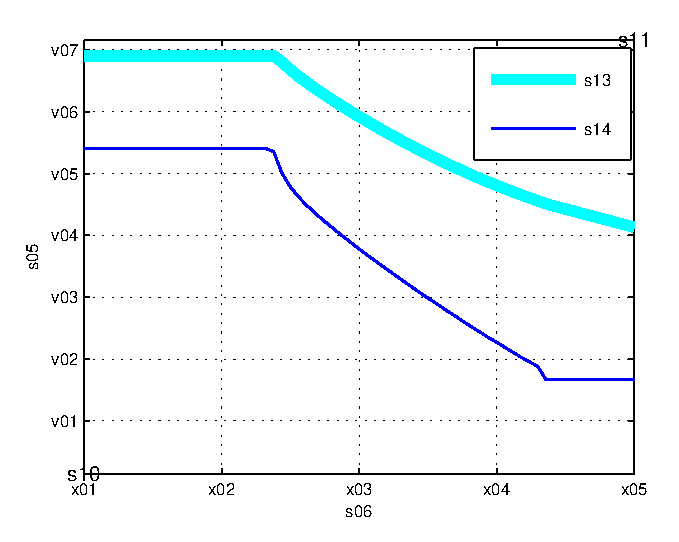
\includegraphics{fig_opt_thr_vs_SNR_AWGN.eps}}%
%\end{psfrags}%
%
% End fig_opt_thr_vs_SNR_AWGN.tex
\end{document}
% See http://www.mathworks.de/matlabcentral/fileexchange/loadFile.do?objectId=4638
% for recent versions of laprint.m.
%
% created by:           LaPrint version 3.16 (13.9.2004)
% created on:           11-Oct-2015 14:32:29
% eps bounding box:     12 cm x 9 cm
% comment:              
%
%\begin{psfrags}%
%\psfragscanon%
%
% text strings:
\psfrag{s05}[b][b]{\fontsize{8}{12}\fontseries{m}\mathversion{normal}\fontshape{n}\selectfont \color[rgb]{0,0,0}\setlength{\tabcolsep}{0pt}\begin{tabular}{c}$\rs(\testpr,  \testpr, \ttsen)$ [bits/sec/Hz]\end{tabular}}%
\psfrag{s06}[t][t]{\fontsize{8}{12}\fontseries{m}\mathversion{normal}\fontshape{n}\selectfont \color[rgb]{0,0,0}\setlength{\tabcolsep}{0pt}\begin{tabular}{c}$\phpth$ [dB]\end{tabular}}%
\psfrag{s10}[][]{\fontsize{10}{15}\fontseries{m}\mathversion{normal}\fontshape{n}\selectfont \color[rgb]{0,0,0}\setlength{\tabcolsep}{0pt}\begin{tabular}{c} \end{tabular}}%
\psfrag{s11}[][]{\fontsize{10}{15}\fontseries{m}\mathversion{normal}\fontshape{n}\selectfont \color[rgb]{0,0,0}\setlength{\tabcolsep}{0pt}\begin{tabular}{c} \end{tabular}}%
\psfrag{s12}[l][l]{\fontsize{8}{12}\fontseries{m}\mathversion{normal}\fontshape{n}\selectfont \color[rgb]{0,0,0}EM}%
\psfrag{s13}[l][l]{\fontsize{8}{12}\fontseries{m}\mathversion{normal}\fontshape{n}\selectfont \color[rgb]{0,0,0}IM}%
\psfrag{s14}[l][l]{\fontsize{8}{12}\fontseries{m}\mathversion{normal}\fontshape{n}\selectfont \color[rgb]{0,0,0}EM}%
%
% axes font properties:
\fontsize{8}{12}\fontseries{m}\mathversion{normal}%
\fontshape{n}\selectfont%
%
% xticklabels:
\psfrag{x01}[t][t]{-110}%
\psfrag{x02}[t][t]{-105}%
\psfrag{x03}[t][t]{-100}%
\psfrag{x04}[t][t]{-95}%
\psfrag{x05}[t][t]{-90}%
%
% yticklabels:
\psfrag{v01}[r][r]{2.2}%
\psfrag{v02}[r][r]{2.4}%
\psfrag{v03}[r][r]{2.6}%
\psfrag{v04}[r][r]{2.8}%
\psfrag{v05}[r][r]{3}%
\psfrag{v06}[r][r]{3.2}%
\psfrag{v07}[r][r]{3.4}%
%
% Figure:
%\resizebox{6cm}{!}{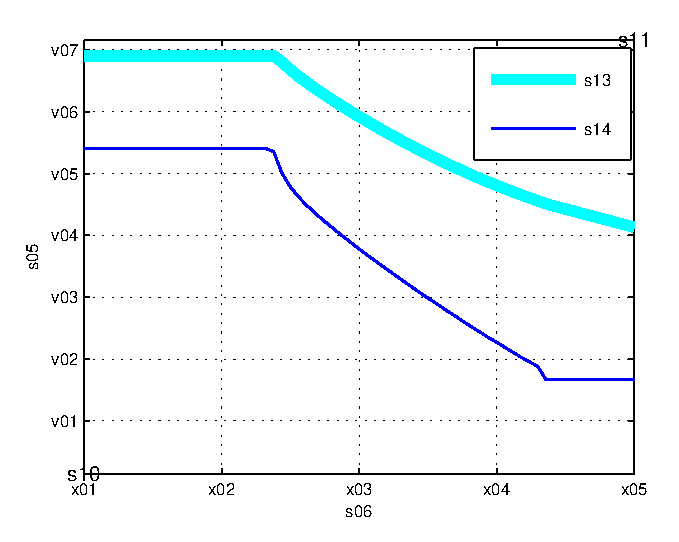
\includegraphics{fig_opt_thr_vs_SNR_AWGN.eps}}%
%\end{psfrags}%
%
% End fig_opt_thr_vs_SNR_AWGN.tex
\end{document}
% See http://www.mathworks.de/matlabcentral/fileexchange/loadFile.do?objectId=4638
% for recent versions of laprint.m.
%
% created by:           LaPrint version 3.16 (13.9.2004)
% created on:           11-Oct-2015 14:32:29
% eps bounding box:     12 cm x 9 cm
% comment:              
%
%\begin{psfrags}%
%\psfragscanon%
%
% text strings:
\psfrag{s05}[b][b]{\fontsize{8}{12}\fontseries{m}\mathversion{normal}\fontshape{n}\selectfont \color[rgb]{0,0,0}\setlength{\tabcolsep}{0pt}\begin{tabular}{c}$\rs(\testpr,  \testpr, \ttsen)$ [bits/sec/Hz]\end{tabular}}%
\psfrag{s06}[t][t]{\fontsize{8}{12}\fontseries{m}\mathversion{normal}\fontshape{n}\selectfont \color[rgb]{0,0,0}\setlength{\tabcolsep}{0pt}\begin{tabular}{c}$\phpth$ [dB]\end{tabular}}%
\psfrag{s10}[][]{\fontsize{10}{15}\fontseries{m}\mathversion{normal}\fontshape{n}\selectfont \color[rgb]{0,0,0}\setlength{\tabcolsep}{0pt}\begin{tabular}{c} \end{tabular}}%
\psfrag{s11}[][]{\fontsize{10}{15}\fontseries{m}\mathversion{normal}\fontshape{n}\selectfont \color[rgb]{0,0,0}\setlength{\tabcolsep}{0pt}\begin{tabular}{c} \end{tabular}}%
\psfrag{s12}[l][l]{\fontsize{8}{12}\fontseries{m}\mathversion{normal}\fontshape{n}\selectfont \color[rgb]{0,0,0}EM}%
\psfrag{s13}[l][l]{\fontsize{8}{12}\fontseries{m}\mathversion{normal}\fontshape{n}\selectfont \color[rgb]{0,0,0}IM}%
\psfrag{s14}[l][l]{\fontsize{8}{12}\fontseries{m}\mathversion{normal}\fontshape{n}\selectfont \color[rgb]{0,0,0}EM}%
%
% axes font properties:
\fontsize{8}{12}\fontseries{m}\mathversion{normal}%
\fontshape{n}\selectfont%
%
% xticklabels:
\psfrag{x01}[t][t]{-110}%
\psfrag{x02}[t][t]{-105}%
\psfrag{x03}[t][t]{-100}%
\psfrag{x04}[t][t]{-95}%
\psfrag{x05}[t][t]{-90}%
%
% yticklabels:
\psfrag{v01}[r][r]{2.2}%
\psfrag{v02}[r][r]{2.4}%
\psfrag{v03}[r][r]{2.6}%
\psfrag{v04}[r][r]{2.8}%
\psfrag{v05}[r][r]{3}%
\psfrag{v06}[r][r]{3.2}%
\psfrag{v07}[r][r]{3.4}%
%
% Figure:
%\resizebox{6cm}{!}{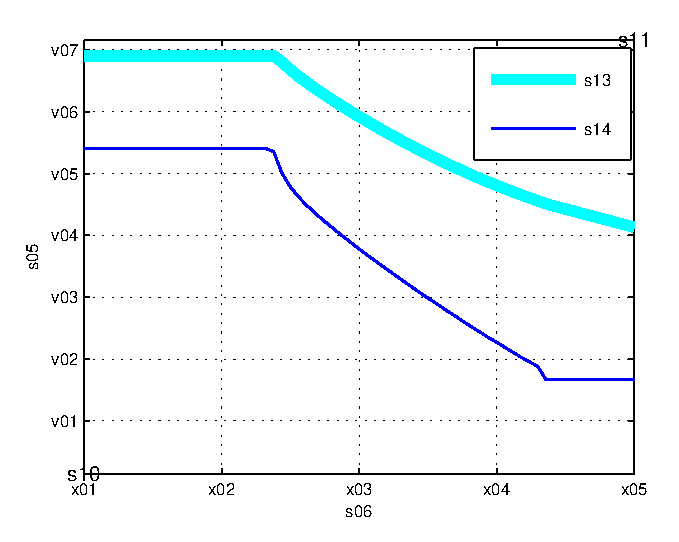
\includegraphics{fig_opt_thr_vs_SNR_AWGN.eps}}%
%\end{psfrags}%
%
% End fig_opt_thr_vs_SNR_AWGN.tex

\centering
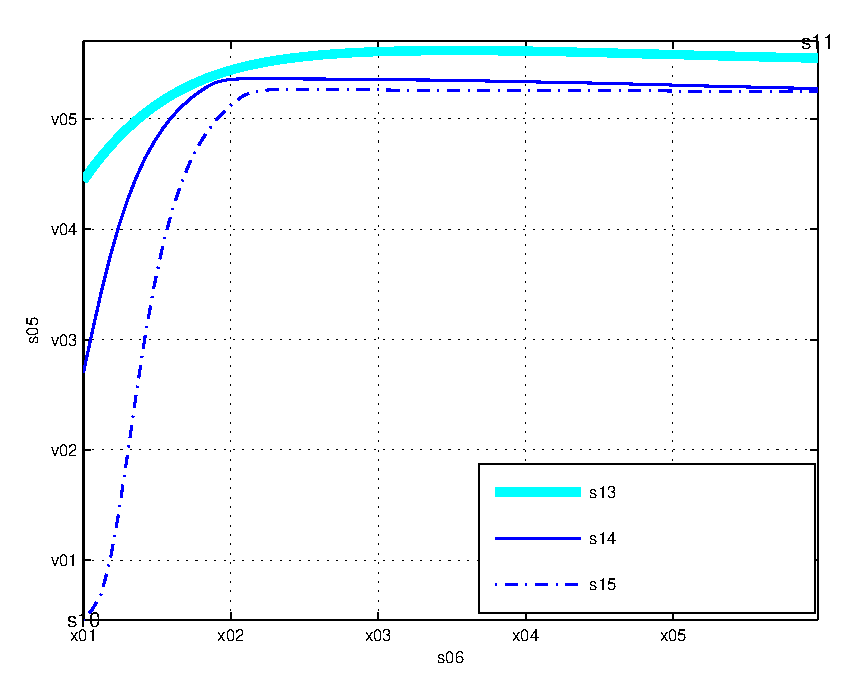
\includegraphics[width= \figscale]{figures/fig_opt_thr_vs_SNR_AWGN}
\caption{\tc{Secondary throughput versus $\snrrcvd$ with $\tau\sub{est} = \SI{5}{ms}$ for the deterministic channel.}}
\label{fig_IS:optT_snr}
%\vspace{-0.7cm}
\end{figure}

Hereafter, the theoretical expressions are considered for the analysis, in addition, the IS is operated at the suitable sensing time. Next, the variation in the achievable throughput $\rs(\test, \ttsen)$ against the received signal to noise ratio $\snrrcvd$ at the ST with $\test = \SI{5}{ms}$ is considered, \tc{refer to} \figurename~\ref{fig_IS:optT_snr}. For $\snrrcvd < -\SI{10}{dB}$, the estimation model incurs a significant performance loss. This clearly reveals that the ideal model overestimates the performance of the IS. \tc{From the previous discussion, it is concluded that the inclusion of the average and the outage constraints (depicted by the proposed framework) precisely tackles the uncertainty in the interference at the PR, arising due to channel estimation, without considerably degrading the performance of the IS.} 


\begin{figure}[!ht]
\centering
\subfloat[]{
%% Add psfrag entries
% This file is generated by the MATLAB m-file laprint.m. It can be included
% into LaTeX documents using the packages graphicx, color and psfrag.
% It is accompanied by a postscript file. A sample LaTeX file is:
%    \documentclass{article}\usepackage{graphicx,color,psfrag}
%    \begin{document}% This file is generated by the MATLAB m-file laprint.m. It can be included
% into LaTeX documents using the packages graphicx, color and psfrag.
% It is accompanied by a postscript file. A sample LaTeX file is:
%    \documentclass{article}\usepackage{graphicx,color,psfrag}
%    \begin{document}% This file is generated by the MATLAB m-file laprint.m. It can be included
% into LaTeX documents using the packages graphicx, color and psfrag.
% It is accompanied by a postscript file. A sample LaTeX file is:
%    \documentclass{article}\usepackage{graphicx,color,psfrag}
%    \begin{document}\input{fig_opt_thr_vs_est_time_sen_time_ac_AWGN}\end{document}
% See http://www.mathworks.de/matlabcentral/fileexchange/loadFile.do?objectId=4638
% for recent versions of laprint.m.
%
% created by:           LaPrint version 3.16 (13.9.2004)
% created on:           11-Nov-2015 10:11:34
% eps bounding box:     16 cm x 12 cm
% comment:              
%
%\begin{psfrags}%
%\psfragscanon%
%
% text strings:
\psfrag{s02}[b][b]{\fontsize{8}{12}\fontseries{m}\mathversion{normal}\fontshape{n}\selectfont \color[rgb]{0,0,0}\setlength{\tabcolsep}{0pt}\begin{tabular}{c}$\trs(\test,\tsen)$ [bits/sec/Hz]\end{tabular}}%
\psfrag{s03}[lt][lt]{\fontsize{8}{12}\fontseries{m}\mathversion{normal}\fontshape{n}\selectfont \color[rgb]{0,0,0}\setlength{\tabcolsep}{0pt}\begin{tabular}{l}$\tsen$ [ms]\end{tabular}}%
\psfrag{s04}[rt][rt]{\fontsize{8}{12}\fontseries{m}\mathversion{normal}\fontshape{n}\selectfont \color[rgb]{0,0,0}\setlength{\tabcolsep}{0pt}\begin{tabular}{r}$\test$ [ms]\end{tabular}}%
%
% axes font properties:
\fontsize{8}{12}\fontseries{m}\mathversion{normal}%
\fontshape{n}\selectfont%
%
% xticklabels:
\psfrag{x01}[t][t]{0}%
\psfrag{x02}[t][t]{5}%
\psfrag{x03}[t][t]{10}%
\psfrag{x04}[t][t]{15}%
\psfrag{x05}[t][t]{20}%
\psfrag{x06}[t][t]{25}%
%
% yticklabels:
\psfrag{v01}[r][r]{0}%
\psfrag{v02}[r][r]{5}%
\psfrag{v03}[r][r]{10}%
%
% zticklabels:
\psfrag{z01}[r][r]{0}%
\psfrag{z02}[r][r]{0.5}%
\psfrag{z03}[r][r]{1}%
\psfrag{z04}[r][r]{1.5}%
\psfrag{z05}[r][r]{2}%
\psfrag{z06}[r][r]{2.5}%
\psfrag{z07}[r][r]{3}%
%
% Figure:
%\resizebox{8cm}{!}{\includegraphics{fig_opt_thr_vs_est_time_sen_time_ac_AWGN.eps}}%
%\end{psfrags}%
%
% End fig_opt_thr_vs_est_time_sen_time_ac_AWGN.tex
\end{document}
% See http://www.mathworks.de/matlabcentral/fileexchange/loadFile.do?objectId=4638
% for recent versions of laprint.m.
%
% created by:           LaPrint version 3.16 (13.9.2004)
% created on:           11-Nov-2015 10:11:34
% eps bounding box:     16 cm x 12 cm
% comment:              
%
%\begin{psfrags}%
%\psfragscanon%
%
% text strings:
\psfrag{s02}[b][b]{\fontsize{8}{12}\fontseries{m}\mathversion{normal}\fontshape{n}\selectfont \color[rgb]{0,0,0}\setlength{\tabcolsep}{0pt}\begin{tabular}{c}$\trs(\test,\tsen)$ [bits/sec/Hz]\end{tabular}}%
\psfrag{s03}[lt][lt]{\fontsize{8}{12}\fontseries{m}\mathversion{normal}\fontshape{n}\selectfont \color[rgb]{0,0,0}\setlength{\tabcolsep}{0pt}\begin{tabular}{l}$\tsen$ [ms]\end{tabular}}%
\psfrag{s04}[rt][rt]{\fontsize{8}{12}\fontseries{m}\mathversion{normal}\fontshape{n}\selectfont \color[rgb]{0,0,0}\setlength{\tabcolsep}{0pt}\begin{tabular}{r}$\test$ [ms]\end{tabular}}%
%
% axes font properties:
\fontsize{8}{12}\fontseries{m}\mathversion{normal}%
\fontshape{n}\selectfont%
%
% xticklabels:
\psfrag{x01}[t][t]{0}%
\psfrag{x02}[t][t]{5}%
\psfrag{x03}[t][t]{10}%
\psfrag{x04}[t][t]{15}%
\psfrag{x05}[t][t]{20}%
\psfrag{x06}[t][t]{25}%
%
% yticklabels:
\psfrag{v01}[r][r]{0}%
\psfrag{v02}[r][r]{5}%
\psfrag{v03}[r][r]{10}%
%
% zticklabels:
\psfrag{z01}[r][r]{0}%
\psfrag{z02}[r][r]{0.5}%
\psfrag{z03}[r][r]{1}%
\psfrag{z04}[r][r]{1.5}%
\psfrag{z05}[r][r]{2}%
\psfrag{z06}[r][r]{2.5}%
\psfrag{z07}[r][r]{3}%
%
% Figure:
%\resizebox{8cm}{!}{\includegraphics{fig_opt_thr_vs_est_time_sen_time_ac_AWGN.eps}}%
%\end{psfrags}%
%
% End fig_opt_thr_vs_est_time_sen_time_ac_AWGN.tex
\end{document}
% See http://www.mathworks.de/matlabcentral/fileexchange/loadFile.do?objectId=4638
% for recent versions of laprint.m.
%
% created by:           LaPrint version 3.16 (13.9.2004)
% created on:           11-Nov-2015 10:11:34
% eps bounding box:     16 cm x 12 cm
% comment:              
%
%\begin{psfrags}%
%\psfragscanon%
%
% text strings:
\psfrag{s02}[b][b]{\fontsize{8}{12}\fontseries{m}\mathversion{normal}\fontshape{n}\selectfont \color[rgb]{0,0,0}\setlength{\tabcolsep}{0pt}\begin{tabular}{c}$\trs(\test,\tsen)$ [bits/sec/Hz]\end{tabular}}%
\psfrag{s03}[lt][lt]{\fontsize{8}{12}\fontseries{m}\mathversion{normal}\fontshape{n}\selectfont \color[rgb]{0,0,0}\setlength{\tabcolsep}{0pt}\begin{tabular}{l}$\tsen$ [ms]\end{tabular}}%
\psfrag{s04}[rt][rt]{\fontsize{8}{12}\fontseries{m}\mathversion{normal}\fontshape{n}\selectfont \color[rgb]{0,0,0}\setlength{\tabcolsep}{0pt}\begin{tabular}{r}$\test$ [ms]\end{tabular}}%
%
% axes font properties:
\fontsize{8}{12}\fontseries{m}\mathversion{normal}%
\fontshape{n}\selectfont%
%
% xticklabels:
\psfrag{x01}[t][t]{0}%
\psfrag{x02}[t][t]{5}%
\psfrag{x03}[t][t]{10}%
\psfrag{x04}[t][t]{15}%
\psfrag{x05}[t][t]{20}%
\psfrag{x06}[t][t]{25}%
%
% yticklabels:
\psfrag{v01}[r][r]{0}%
\psfrag{v02}[r][r]{5}%
\psfrag{v03}[r][r]{10}%
%
% zticklabels:
\psfrag{z01}[r][r]{0}%
\psfrag{z02}[r][r]{0.5}%
\psfrag{z03}[r][r]{1}%
\psfrag{z04}[r][r]{1.5}%
\psfrag{z05}[r][r]{2}%
\psfrag{z06}[r][r]{2.5}%
\psfrag{z07}[r][r]{3}%
%
% Figure:
%\resizebox{8cm}{!}{\includegraphics{fig_opt_thr_vs_est_time_sen_time_ac_AWGN.eps}}%
%\end{psfrags}%
%
% End fig_opt_thr_vs_est_time_sen_time_ac_AWGN.tex

\centering
\begin{tikzpicture}[scale=1]
\node[anchor=south west,inner sep=0] (image) at (0,0)
{
\includegraphics[width= \figscale]{figures/fig_opt_thr_vs_est_time_sen_time_ac_AWGN}
};
\begin{scope}[x={(image.south east)},y={(image.north west)}]
%\draw[black,->] (0.6,0.44) node[above=0.0,  font=\scriptsize] {$\mpd \in \{0.05,0.10,0.15\}$} -- (0.56,0.33);
\draw[black,->] (0.389,0.83) -- (0.389,0.656);
\node[draw=none, font=\scriptsize] at (0.389, 0.86) {$\rs(\ttest, \ttsen)$};
 
%\draw[help lines,xstep=.1,ystep=.1] (0,0) grid (1,1);
%\foreach \x in {0,1,...,9} { \node [anchor=north] at (\x/10,0) {0.\x}; }
%\foreach \y in {0,1,...,9} { \node [anchor=east] at (0,\y/10) {0.\y}; }
\end{scope}
\end{tikzpicture}

\label{fig_IS:EST_ac}}
\hfil
\subfloat[]{
%% Add psfrag entries
% This file is generated by the MATLAB m-file laprint.m. It can be included
% into LaTeX documents using the packages graphicx, color and psfrag.
% It is accompanied by a postscript file. A sample LaTeX file is:
%    \documentclass{article}\usepackage{graphicx,color,psfrag}
%    \begin{document}% This file is generated by the MATLAB m-file laprint.m. It can be included
% into LaTeX documents using the packages graphicx, color and psfrag.
% It is accompanied by a postscript file. A sample LaTeX file is:
%    \documentclass{article}\usepackage{graphicx,color,psfrag}
%    \begin{document}% This file is generated by the MATLAB m-file laprint.m. It can be included
% into LaTeX documents using the packages graphicx, color and psfrag.
% It is accompanied by a postscript file. A sample LaTeX file is:
%    \documentclass{article}\usepackage{graphicx,color,psfrag}
%    \begin{document}\input{fig_opt_thr_vs_est_time_sen_time_oc_AWGN}\end{document}
% See http://www.mathworks.de/matlabcentral/fileexchange/loadFile.do?objectId=4638
% for recent versions of laprint.m.
%
% created by:           LaPrint version 3.16 (13.9.2004)
% created on:           11-Nov-2015 10:11:33
% eps bounding box:     16 cm x 12 cm
% comment:              
%
%\begin{psfrags}%
%\psfragscanon%
%
% text strings:
\psfrag{s02}[b][b]{\fontsize{8}{12}\fontseries{m}\mathversion{normal}\fontshape{n}\selectfont \color[rgb]{0,0,0}\setlength{\tabcolsep}{0pt}\begin{tabular}{c}$\trs(\test,\tsen)$ [bits/sec/Hz]\end{tabular}}%
\psfrag{s03}[lt][lt]{\fontsize{8}{12}\fontseries{m}\mathversion{normal}\fontshape{n}\selectfont \color[rgb]{0,0,0}\setlength{\tabcolsep}{0pt}\begin{tabular}{l}$\tsen$ [ms]\end{tabular}}%
\psfrag{s04}[rt][rt]{\fontsize{8}{12}\fontseries{m}\mathversion{normal}\fontshape{n}\selectfont \color[rgb]{0,0,0}\setlength{\tabcolsep}{0pt}\begin{tabular}{r}$\test$ [ms]\end{tabular}}%
%
% axes font properties:
\fontsize{8}{12}\fontseries{m}\mathversion{normal}%
\fontshape{n}\selectfont%
%
% xticklabels:
\psfrag{x01}[t][t]{0}%
\psfrag{x02}[t][t]{5}%
\psfrag{x03}[t][t]{10}%
\psfrag{x04}[t][t]{15}%
\psfrag{x05}[t][t]{20}%
\psfrag{x06}[t][t]{25}%
%
% yticklabels:
\psfrag{v01}[r][r]{0}%
\psfrag{v02}[r][r]{5}%
\psfrag{v03}[r][r]{10}%
%
% zticklabels:
\psfrag{z01}[r][r]{0}%
\psfrag{z02}[r][r]{0.5}%
\psfrag{z03}[r][r]{1}%
\psfrag{z04}[r][r]{1.5}%
\psfrag{z05}[r][r]{2}%
\psfrag{z06}[r][r]{2.5}%
\psfrag{z07}[r][r]{3}%
%
% Figure:
%\resizebox{8cm}{!}{\includegraphics{fig_opt_thr_vs_est_time_sen_time_oc_AWGN.eps}}%
%\end{psfrags}%
%
% End fig_opt_thr_vs_est_time_sen_time_oc_AWGN.tex
\end{document}
% See http://www.mathworks.de/matlabcentral/fileexchange/loadFile.do?objectId=4638
% for recent versions of laprint.m.
%
% created by:           LaPrint version 3.16 (13.9.2004)
% created on:           11-Nov-2015 10:11:33
% eps bounding box:     16 cm x 12 cm
% comment:              
%
%\begin{psfrags}%
%\psfragscanon%
%
% text strings:
\psfrag{s02}[b][b]{\fontsize{8}{12}\fontseries{m}\mathversion{normal}\fontshape{n}\selectfont \color[rgb]{0,0,0}\setlength{\tabcolsep}{0pt}\begin{tabular}{c}$\trs(\test,\tsen)$ [bits/sec/Hz]\end{tabular}}%
\psfrag{s03}[lt][lt]{\fontsize{8}{12}\fontseries{m}\mathversion{normal}\fontshape{n}\selectfont \color[rgb]{0,0,0}\setlength{\tabcolsep}{0pt}\begin{tabular}{l}$\tsen$ [ms]\end{tabular}}%
\psfrag{s04}[rt][rt]{\fontsize{8}{12}\fontseries{m}\mathversion{normal}\fontshape{n}\selectfont \color[rgb]{0,0,0}\setlength{\tabcolsep}{0pt}\begin{tabular}{r}$\test$ [ms]\end{tabular}}%
%
% axes font properties:
\fontsize{8}{12}\fontseries{m}\mathversion{normal}%
\fontshape{n}\selectfont%
%
% xticklabels:
\psfrag{x01}[t][t]{0}%
\psfrag{x02}[t][t]{5}%
\psfrag{x03}[t][t]{10}%
\psfrag{x04}[t][t]{15}%
\psfrag{x05}[t][t]{20}%
\psfrag{x06}[t][t]{25}%
%
% yticklabels:
\psfrag{v01}[r][r]{0}%
\psfrag{v02}[r][r]{5}%
\psfrag{v03}[r][r]{10}%
%
% zticklabels:
\psfrag{z01}[r][r]{0}%
\psfrag{z02}[r][r]{0.5}%
\psfrag{z03}[r][r]{1}%
\psfrag{z04}[r][r]{1.5}%
\psfrag{z05}[r][r]{2}%
\psfrag{z06}[r][r]{2.5}%
\psfrag{z07}[r][r]{3}%
%
% Figure:
%\resizebox{8cm}{!}{\includegraphics{fig_opt_thr_vs_est_time_sen_time_oc_AWGN.eps}}%
%\end{psfrags}%
%
% End fig_opt_thr_vs_est_time_sen_time_oc_AWGN.tex
\end{document}
% See http://www.mathworks.de/matlabcentral/fileexchange/loadFile.do?objectId=4638
% for recent versions of laprint.m.
%
% created by:           LaPrint version 3.16 (13.9.2004)
% created on:           11-Nov-2015 10:11:33
% eps bounding box:     16 cm x 12 cm
% comment:              
%
%\begin{psfrags}%
%\psfragscanon%
%
% text strings:
\psfrag{s02}[b][b]{\fontsize{8}{12}\fontseries{m}\mathversion{normal}\fontshape{n}\selectfont \color[rgb]{0,0,0}\setlength{\tabcolsep}{0pt}\begin{tabular}{c}$\trs(\test,\tsen)$ [bits/sec/Hz]\end{tabular}}%
\psfrag{s03}[lt][lt]{\fontsize{8}{12}\fontseries{m}\mathversion{normal}\fontshape{n}\selectfont \color[rgb]{0,0,0}\setlength{\tabcolsep}{0pt}\begin{tabular}{l}$\tsen$ [ms]\end{tabular}}%
\psfrag{s04}[rt][rt]{\fontsize{8}{12}\fontseries{m}\mathversion{normal}\fontshape{n}\selectfont \color[rgb]{0,0,0}\setlength{\tabcolsep}{0pt}\begin{tabular}{r}$\test$ [ms]\end{tabular}}%
%
% axes font properties:
\fontsize{8}{12}\fontseries{m}\mathversion{normal}%
\fontshape{n}\selectfont%
%
% xticklabels:
\psfrag{x01}[t][t]{0}%
\psfrag{x02}[t][t]{5}%
\psfrag{x03}[t][t]{10}%
\psfrag{x04}[t][t]{15}%
\psfrag{x05}[t][t]{20}%
\psfrag{x06}[t][t]{25}%
%
% yticklabels:
\psfrag{v01}[r][r]{0}%
\psfrag{v02}[r][r]{5}%
\psfrag{v03}[r][r]{10}%
%
% zticklabels:
\psfrag{z01}[r][r]{0}%
\psfrag{z02}[r][r]{0.5}%
\psfrag{z03}[r][r]{1}%
\psfrag{z04}[r][r]{1.5}%
\psfrag{z05}[r][r]{2}%
\psfrag{z06}[r][r]{2.5}%
\psfrag{z07}[r][r]{3}%
%
% Figure:
%\resizebox{8cm}{!}{\includegraphics{fig_opt_thr_vs_est_time_sen_time_oc_AWGN.eps}}%
%\end{psfrags}%
%
% End fig_opt_thr_vs_est_time_sen_time_oc_AWGN.tex

\centering
\begin{tikzpicture}[scale=1]
\node[anchor=south west,inner sep=0] (image) at (0,0)
{
\includegraphics[width= \figscale]{figures/fig_opt_thr_vs_est_time_sen_time_oc_AWGN}
};
\begin{scope}[x={(image.south east)},y={(image.north west)}]
%\draw[black,->] (0.6,0.44) node[above=0.0,  font=\scriptsize] {$\mpd \in \{0.05,0.10,0.15\}$} -- (0.56,0.33);
\draw[black,->] (0.353,0.83) -- (0.353,0.699);
\node[draw=none, font=\scriptsize] at (0.353, 0.86) {$\rs(\ttest, \ttsen)$};
 
%\draw[help lines,xstep=.1,ystep=.1] (0,0) grid (1,1);
%\foreach \x in {0,1,...,9} { \node [anchor=north] at (\x/10,0) {0.\x}; }
%\foreach \y in {0,1,...,9} { \node [anchor=east] at (0,\y/10) {0.\y}; }
\end{scope}
\end{tikzpicture}
\label{fig_IS:EST_oc}}
\vspace{4mm}
\caption{\tc{Estimation-sensing-throughput tradeoff for the estimation model for (a) average constraint and (b) outage constraint with $\mpd = 0.05$.}}
\label{fig_IS:EST}
%\vspace{-0.7cm}
\end{figure}


Upon maximizing the secondary throughput, it is interesting to analyze the variation of the secondary throughput with the estimation time. Corresponding to the estimation model, \figurename~\ref{fig_IS:EST} illustrates a tradeoff among the estimation time, the sensing time and the secondary throughput, \tc{refer to} Remark \ref{rem_IS:rem1}. \tc{From \figurename~\ref{fig_IS:EST}, it can be noticed that the function $\rs(\test, \tsen)$ is well-behaved in the region $0 < \test \le \tsen \le T$ and consists of a global maximum, yielding the achievable secondary throughput. 

This tradeoff depicted by the proposed framework, further presented in \figurename~\ref{fig_IS:optT_test}, can be explained from the fact that low values of the estimation time result in large variations in $\epd$.} To counteract and satisfy the average and the outage constraints, the corresponding thresholds shift to a lower value. This causes an increase in $\pfa$, thereby increasing the sensing-throughput curvature. As a result, the suitable sensing time is obtained at a higher value. However, beyond a certain value ($\ttest$), a further increase in the estimation time slightly contributes to the performance improvement and largely consumes the time resources. As a consequence to the estimation-sensing-throughput tradeoff, the suitable estimation time that yields an achievable throughput $\trs(\ttest,\ttsen)$ is determined. 

\begin{figure}[!t]

%% Add psfrag entries
% This file is generated by the MATLAB m-file laprint.m. It can be included
% into LaTeX documents using the packages graphicx, color and psfrag.
% It is accompanied by a postscript file. A sample LaTeX file is:
%    \documentclass{article}\usepackage{graphicx,color,psfrag}
%    \begin{document}% This file is generated by the MATLAB m-file laprint.m. It can be included
% into LaTeX documents using the packages graphicx, color and psfrag.
% It is accompanied by a postscript file. A sample LaTeX file is:
%    \documentclass{article}\usepackage{graphicx,color,psfrag}
%    \begin{document}% This file is generated by the MATLAB m-file laprint.m. It can be included
% into LaTeX documents using the packages graphicx, color and psfrag.
% It is accompanied by a postscript file. A sample LaTeX file is:
%    \documentclass{article}\usepackage{graphicx,color,psfrag}
%    \begin{document}\input{fig_opt_thr_vs_est_time_diff_mu_AWGN}\end{document}
% See http://www.mathworks.de/matlabcentral/fileexchange/loadFile.do?objectId=4638
% for recent versions of laprint.m.
%
% created by:           LaPrint version 3.16 (13.9.2004)
% created on:           12-Jul-2016 15:03:36
% eps bounding box:     16 cm x 12 cm
% comment:              
%
%\begin{psfrags}%
%\psfragscanon%
%
% text strings:
\psfrag{s05}[b][b]{\fontsize{8}{12}\fontseries{m}\mathversion{normal}\fontshape{n}\selectfont \color[rgb]{0,0,0}\setlength{\tabcolsep}{0pt}\begin{tabular}{c}$\trs(\test,\ttsen)$ [bits/sec/Hz]\end{tabular}}%
\psfrag{s06}[t][t]{\fontsize{8}{12}\fontseries{m}\mathversion{normal}\fontshape{n}\selectfont \color[rgb]{0,0,0}\setlength{\tabcolsep}{0pt}\begin{tabular}{c}$\test$ [ms]\end{tabular}}%
\psfrag{s10}[][]{\fontsize{10}{15}\fontseries{m}\mathversion{normal}\fontshape{n}\selectfont \color[rgb]{0,0,0}\setlength{\tabcolsep}{0pt}\begin{tabular}{c} \end{tabular}}%
\psfrag{s11}[][]{\fontsize{10}{15}\fontseries{m}\mathversion{normal}\fontshape{n}\selectfont \color[rgb]{0,0,0}\setlength{\tabcolsep}{0pt}\begin{tabular}{c} \end{tabular}}%
\psfrag{s12}[l][l]{\fontsize{8}{12}\fontseries{m}\mathversion{normal}\fontshape{n}\selectfont \color[rgb]{0,0,0}$\trs(\ttest,\ttsen)$}%
\psfrag{s13}[l][l]{\fontsize{8}{12}\fontseries{m}\mathversion{normal}\fontshape{n}\selectfont \color[rgb]{0,0,0}IM}%
\psfrag{s14}[l][l]{\fontsize{8}{12}\fontseries{m}\mathversion{normal}\fontshape{n}\selectfont \color[rgb]{0,0,0}EM-AC, Problem 1}%
\psfrag{s15}[l][l]{\fontsize{8}{12}\fontseries{m}\mathversion{normal}\fontshape{n}\selectfont \color[rgb]{0,0,0}EM-OC, Problem 2}%
\psfrag{s16}[l][l]{\fontsize{8}{12}\fontseries{m}\mathversion{normal}\fontshape{n}\selectfont \color[rgb]{0,0,0}Corollary 1}%
\psfrag{s17}[l][l]{\fontsize{8}{12}\fontseries{m}\mathversion{normal}\fontshape{n}\selectfont \color[rgb]{0,0,0}$\trs(\ttest,\ttsen)$}%
%
% axes font properties:
\fontsize{8}{12}\fontseries{m}\mathversion{normal}%
\fontshape{n}\selectfont%
%
% xticklabels:
\psfrag{x01}[t][t]{1}%
\psfrag{x02}[t][t]{2}%
\psfrag{x03}[t][t]{3}%
\psfrag{x04}[t][t]{4}%
\psfrag{x05}[t][t]{5}%
\psfrag{x06}[t][t]{6}%
\psfrag{x07}[t][t]{7}%
\psfrag{x08}[t][t]{8}%
\psfrag{x09}[t][t]{9}%
\psfrag{x10}[t][t]{10}%
%
% yticklabels:
\psfrag{v01}[r][r]{1.8}%
\psfrag{v02}[r][r]{1.9}%
\psfrag{v03}[r][r]{2}%
\psfrag{v04}[r][r]{2.1}%
\psfrag{v05}[r][r]{2.2}%
\psfrag{v06}[r][r]{2.3}%
\psfrag{v07}[r][r]{2.4}%
\psfrag{v08}[r][r]{2.5}%
\psfrag{v09}[r][r]{2.6}%
\psfrag{v10}[r][r]{2.7}%
%
% Figure:
%\resizebox{8cm}{!}{\includegraphics{fig_opt_thr_vs_est_time_diff_mu_AWGN.eps}}%
%\end{psfrags}%
%
% End fig_opt_thr_vs_est_time_diff_mu_AWGN.tex
\end{document}
% See http://www.mathworks.de/matlabcentral/fileexchange/loadFile.do?objectId=4638
% for recent versions of laprint.m.
%
% created by:           LaPrint version 3.16 (13.9.2004)
% created on:           12-Jul-2016 15:03:36
% eps bounding box:     16 cm x 12 cm
% comment:              
%
%\begin{psfrags}%
%\psfragscanon%
%
% text strings:
\psfrag{s05}[b][b]{\fontsize{8}{12}\fontseries{m}\mathversion{normal}\fontshape{n}\selectfont \color[rgb]{0,0,0}\setlength{\tabcolsep}{0pt}\begin{tabular}{c}$\trs(\test,\ttsen)$ [bits/sec/Hz]\end{tabular}}%
\psfrag{s06}[t][t]{\fontsize{8}{12}\fontseries{m}\mathversion{normal}\fontshape{n}\selectfont \color[rgb]{0,0,0}\setlength{\tabcolsep}{0pt}\begin{tabular}{c}$\test$ [ms]\end{tabular}}%
\psfrag{s10}[][]{\fontsize{10}{15}\fontseries{m}\mathversion{normal}\fontshape{n}\selectfont \color[rgb]{0,0,0}\setlength{\tabcolsep}{0pt}\begin{tabular}{c} \end{tabular}}%
\psfrag{s11}[][]{\fontsize{10}{15}\fontseries{m}\mathversion{normal}\fontshape{n}\selectfont \color[rgb]{0,0,0}\setlength{\tabcolsep}{0pt}\begin{tabular}{c} \end{tabular}}%
\psfrag{s12}[l][l]{\fontsize{8}{12}\fontseries{m}\mathversion{normal}\fontshape{n}\selectfont \color[rgb]{0,0,0}$\trs(\ttest,\ttsen)$}%
\psfrag{s13}[l][l]{\fontsize{8}{12}\fontseries{m}\mathversion{normal}\fontshape{n}\selectfont \color[rgb]{0,0,0}IM}%
\psfrag{s14}[l][l]{\fontsize{8}{12}\fontseries{m}\mathversion{normal}\fontshape{n}\selectfont \color[rgb]{0,0,0}EM-AC, Problem 1}%
\psfrag{s15}[l][l]{\fontsize{8}{12}\fontseries{m}\mathversion{normal}\fontshape{n}\selectfont \color[rgb]{0,0,0}EM-OC, Problem 2}%
\psfrag{s16}[l][l]{\fontsize{8}{12}\fontseries{m}\mathversion{normal}\fontshape{n}\selectfont \color[rgb]{0,0,0}Corollary 1}%
\psfrag{s17}[l][l]{\fontsize{8}{12}\fontseries{m}\mathversion{normal}\fontshape{n}\selectfont \color[rgb]{0,0,0}$\trs(\ttest,\ttsen)$}%
%
% axes font properties:
\fontsize{8}{12}\fontseries{m}\mathversion{normal}%
\fontshape{n}\selectfont%
%
% xticklabels:
\psfrag{x01}[t][t]{1}%
\psfrag{x02}[t][t]{2}%
\psfrag{x03}[t][t]{3}%
\psfrag{x04}[t][t]{4}%
\psfrag{x05}[t][t]{5}%
\psfrag{x06}[t][t]{6}%
\psfrag{x07}[t][t]{7}%
\psfrag{x08}[t][t]{8}%
\psfrag{x09}[t][t]{9}%
\psfrag{x10}[t][t]{10}%
%
% yticklabels:
\psfrag{v01}[r][r]{1.8}%
\psfrag{v02}[r][r]{1.9}%
\psfrag{v03}[r][r]{2}%
\psfrag{v04}[r][r]{2.1}%
\psfrag{v05}[r][r]{2.2}%
\psfrag{v06}[r][r]{2.3}%
\psfrag{v07}[r][r]{2.4}%
\psfrag{v08}[r][r]{2.5}%
\psfrag{v09}[r][r]{2.6}%
\psfrag{v10}[r][r]{2.7}%
%
% Figure:
%\resizebox{8cm}{!}{\includegraphics{fig_opt_thr_vs_est_time_diff_mu_AWGN.eps}}%
%\end{psfrags}%
%
% End fig_opt_thr_vs_est_time_diff_mu_AWGN.tex
\end{document}
% See http://www.mathworks.de/matlabcentral/fileexchange/loadFile.do?objectId=4638
% for recent versions of laprint.m.
%
% created by:           LaPrint version 3.16 (13.9.2004)
% created on:           12-Jul-2016 15:03:36
% eps bounding box:     16 cm x 12 cm
% comment:              
%
%\begin{psfrags}%
%\psfragscanon%
%
% text strings:
\psfrag{s05}[b][b]{\fontsize{8}{12}\fontseries{m}\mathversion{normal}\fontshape{n}\selectfont \color[rgb]{0,0,0}\setlength{\tabcolsep}{0pt}\begin{tabular}{c}$\trs(\test,\ttsen)$ [bits/sec/Hz]\end{tabular}}%
\psfrag{s06}[t][t]{\fontsize{8}{12}\fontseries{m}\mathversion{normal}\fontshape{n}\selectfont \color[rgb]{0,0,0}\setlength{\tabcolsep}{0pt}\begin{tabular}{c}$\test$ [ms]\end{tabular}}%
\psfrag{s10}[][]{\fontsize{10}{15}\fontseries{m}\mathversion{normal}\fontshape{n}\selectfont \color[rgb]{0,0,0}\setlength{\tabcolsep}{0pt}\begin{tabular}{c} \end{tabular}}%
\psfrag{s11}[][]{\fontsize{10}{15}\fontseries{m}\mathversion{normal}\fontshape{n}\selectfont \color[rgb]{0,0,0}\setlength{\tabcolsep}{0pt}\begin{tabular}{c} \end{tabular}}%
\psfrag{s12}[l][l]{\fontsize{8}{12}\fontseries{m}\mathversion{normal}\fontshape{n}\selectfont \color[rgb]{0,0,0}$\trs(\ttest,\ttsen)$}%
\psfrag{s13}[l][l]{\fontsize{8}{12}\fontseries{m}\mathversion{normal}\fontshape{n}\selectfont \color[rgb]{0,0,0}IM}%
\psfrag{s14}[l][l]{\fontsize{8}{12}\fontseries{m}\mathversion{normal}\fontshape{n}\selectfont \color[rgb]{0,0,0}EM-AC, Problem 1}%
\psfrag{s15}[l][l]{\fontsize{8}{12}\fontseries{m}\mathversion{normal}\fontshape{n}\selectfont \color[rgb]{0,0,0}EM-OC, Problem 2}%
\psfrag{s16}[l][l]{\fontsize{8}{12}\fontseries{m}\mathversion{normal}\fontshape{n}\selectfont \color[rgb]{0,0,0}Corollary 1}%
\psfrag{s17}[l][l]{\fontsize{8}{12}\fontseries{m}\mathversion{normal}\fontshape{n}\selectfont \color[rgb]{0,0,0}$\trs(\ttest,\ttsen)$}%
%
% axes font properties:
\fontsize{8}{12}\fontseries{m}\mathversion{normal}%
\fontshape{n}\selectfont%
%
% xticklabels:
\psfrag{x01}[t][t]{1}%
\psfrag{x02}[t][t]{2}%
\psfrag{x03}[t][t]{3}%
\psfrag{x04}[t][t]{4}%
\psfrag{x05}[t][t]{5}%
\psfrag{x06}[t][t]{6}%
\psfrag{x07}[t][t]{7}%
\psfrag{x08}[t][t]{8}%
\psfrag{x09}[t][t]{9}%
\psfrag{x10}[t][t]{10}%
%
% yticklabels:
\psfrag{v01}[r][r]{1.8}%
\psfrag{v02}[r][r]{1.9}%
\psfrag{v03}[r][r]{2}%
\psfrag{v04}[r][r]{2.1}%
\psfrag{v05}[r][r]{2.2}%
\psfrag{v06}[r][r]{2.3}%
\psfrag{v07}[r][r]{2.4}%
\psfrag{v08}[r][r]{2.5}%
\psfrag{v09}[r][r]{2.6}%
\psfrag{v10}[r][r]{2.7}%
%
% Figure:
%\resizebox{8cm}{!}{\includegraphics{fig_opt_thr_vs_est_time_diff_mu_AWGN.eps}}%
%\end{psfrags}%
%
% End fig_opt_thr_vs_est_time_diff_mu_AWGN.tex

\centering
\begin{tikzpicture}[scale=1]
\node[anchor=south west,inner sep=0] (image) at (0,0)
{
\includegraphics[width= \figscale]{figures/fig_opt_thr_vs_est_time_diff_mu_AWGN}
};
\begin{scope}[x={(image.south east)},y={(image.north west)}]
\draw[black,->] (0.25,0.64) -- (0.18,0.84);
\node[draw=none, font=\scriptsize] at (0.35, 0.58) {$\mpd \in \{0.05,0.10,0.15\}$};
 
%\draw[black,->] (0.25,0.6) node[below =12.0,right=-20.0,  font=\scriptsize] {$\mpd \in \{0.05,0.10,0.15\}$} -- (0.18,0.8);

%\draw[help lines,xstep=.1,ystep=.1] (0,0) grid (1,1);
%\foreach \x in {0,1,...,9} { \node [anchor=north] at (\x/10,0) {0.\x}; }
%\foreach \y in {0,1,...,9} { \node [anchor=east] at (0,\y/10) {0.\y}; }
\end{scope}
\end{tikzpicture}

\caption{\tc{Estimation-sensing-throughput tradeoff for the average and the outage constraints with $\snrrcvd = \SI{-10}{dB}$, where the secondary throughput is maximized over the sensing time, $\trs(\test,\ttsen)$.}} %The estimation-sensing-throughput tradeoff is utilized to determine a suitable estimation time $\ttest$ that maximizes the throughput, $\trs(\ttest,\ttsen)$.}}
\label{fig_IS:optT_test}
%\vspace{-0.7cm}
\end{figure}

Besides that, the variation in the secondary throughput for different values of the outage constraint is illustrated, refer to \figurename~\ref{fig_IS:optT_test}. It is observed that for the selected choice of $\mpd$, the outage constraint is severe as compared to the average constraint, hence, results in a lower secondary throughput or achieves a greater performance degradation. Thus, depending on the nature of the policy (aggressive or conservative) followed by the regulatory bodies towards the interference at the primary system, it is possible to define $\mpd$ accordingly during the system design. \tc{Moreover, it is observed that the alternative approach proposed in Corollary \ref{cor_IS:cor1} does not present any noticeable performance difference depicted in terms of the achievable throughput corresponding to the one characterized in Problems \ref{th_IS:th1} and \ref{th_IS:th2}. 
}

\begin{figure}[!ht]
\centering
%\subfloat[]{
% This file is generated by the MATLAB m-file laprint.m. It can be included
% into LaTeX documents using the packages graphicx, color and psfrag.
% It is accompanied by a postscript file. A sample LaTeX file is:
%    \documentclass{article}\usepackage{graphicx,color,psfrag}
%    \begin{document}% This file is generated by the MATLAB m-file laprint.m. It can be included
% into LaTeX documents using the packages graphicx, color and psfrag.
% It is accompanied by a postscript file. A sample LaTeX file is:
%    \documentclass{article}\usepackage{graphicx,color,psfrag}
%    \begin{document}% This file is generated by the MATLAB m-file laprint.m. It can be included
% into LaTeX documents using the packages graphicx, color and psfrag.
% It is accompanied by a postscript file. A sample LaTeX file is:
%    \documentclass{article}\usepackage{graphicx,color,psfrag}
%    \begin{document}\input{fig_P_d_vs_est_time_diff_mu_AWGN}\end{document}
% See http://www.mathworks.de/matlabcentral/fileexchange/loadFile.do?objectId=4638
% for recent versions of laprint.m.
%
% created by:           LaPrint version 3.16 (13.9.2004)
% created on:           10-Nov-2015 13:50:43
% eps bounding box:     16 cm x 12 cm
% comment:              
%
%\begin{psfrags}%
%\psfragscanon%
%
% text strings:
\psfrag{s05}[b][b]{\fontsize{8}{12}\fontseries{m}\mathversion{normal}\fontshape{n}\selectfont \color[rgb]{0,0,0}\setlength{\tabcolsep}{0pt}\begin{tabular}{c}$\e{\pd}{\pd}$\end{tabular}}%
\psfrag{s06}[t][t]{\fontsize{8}{12}\fontseries{m}\mathversion{normal}\fontshape{n}\selectfont \color[rgb]{0,0,0}\setlength{\tabcolsep}{0pt}\begin{tabular}{c}$\test$ [ms]\end{tabular}}%
\psfrag{s10}[][]{\fontsize{10}{15}\fontseries{m}\mathversion{normal}\fontshape{n}\selectfont \color[rgb]{0,0,0}\setlength{\tabcolsep}{0pt}\begin{tabular}{c} \end{tabular}}%
\psfrag{s11}[][]{\fontsize{10}{15}\fontseries{m}\mathversion{normal}\fontshape{n}\selectfont \color[rgb]{0,0,0}\setlength{\tabcolsep}{0pt}\begin{tabular}{c} \end{tabular}}%
\psfrag{s12}[l][l]{\fontsize{8}{12}\fontseries{m}\mathversion{normal}\fontshape{n}\selectfont \color[rgb]{0,0,0}Corollary 1}%
\psfrag{s13}[l][l]{\fontsize{8}{12}\fontseries{m}\mathversion{normal}\fontshape{n}\selectfont \color[rgb]{0,0,0}IM}%
\psfrag{s14}[l][l]{\fontsize{8}{12}\fontseries{m}\mathversion{normal}\fontshape{n}\selectfont \color[rgb]{0,0,0}EM-AC, Thm. 1}%
\psfrag{s15}[l][l]{\fontsize{8}{12}\fontseries{m}\mathversion{normal}\fontshape{n}\selectfont \color[rgb]{0,0,0}EM-OC, Thm. 2}%
\psfrag{s16}[l][l]{\fontsize{8}{12}\fontseries{m}\mathversion{normal}\fontshape{n}\selectfont \color[rgb]{0,0,0}Corollary 1}%
%
% axes font properties:
\fontsize{8}{12}\fontseries{m}\mathversion{normal}%
\fontshape{n}\selectfont%
%
% xticklabels:
\psfrag{x01}[t][t]{1}%
\psfrag{x02}[t][t]{2}%
\psfrag{x03}[t][t]{3}%
\psfrag{x04}[t][t]{4}%
\psfrag{x05}[t][t]{5}%
\psfrag{x06}[t][t]{6}%
\psfrag{x07}[t][t]{7}%
\psfrag{x08}[t][t]{8}%
\psfrag{x09}[t][t]{9}%
\psfrag{x10}[t][t]{10}%
%
% yticklabels:
\psfrag{v01}[r][r]{0.8}%
\psfrag{v02}[r][r]{0.82}%
\psfrag{v03}[r][r]{0.84}%
\psfrag{v04}[r][r]{0.86}%
\psfrag{v05}[r][r]{0.88}%
\psfrag{v06}[r][r]{0.9}%
\psfrag{v07}[r][r]{0.92}%
\psfrag{v08}[r][r]{0.94}%
\psfrag{v09}[r][r]{0.96}%
\psfrag{v10}[r][r]{0.98}%
\psfrag{v11}[r][r]{1}%
%
% Figure:
%\resizebox{8cm}{!}{\includegraphics{fig_P_d_vs_est_time_diff_mu_AWGN.eps}}%
%\end{psfrags}%
%
% End fig_P_d_vs_est_time_diff_mu_AWGN.tex
\end{document}
% See http://www.mathworks.de/matlabcentral/fileexchange/loadFile.do?objectId=4638
% for recent versions of laprint.m.
%
% created by:           LaPrint version 3.16 (13.9.2004)
% created on:           10-Nov-2015 13:50:43
% eps bounding box:     16 cm x 12 cm
% comment:              
%
%\begin{psfrags}%
%\psfragscanon%
%
% text strings:
\psfrag{s05}[b][b]{\fontsize{8}{12}\fontseries{m}\mathversion{normal}\fontshape{n}\selectfont \color[rgb]{0,0,0}\setlength{\tabcolsep}{0pt}\begin{tabular}{c}$\e{\pd}{\pd}$\end{tabular}}%
\psfrag{s06}[t][t]{\fontsize{8}{12}\fontseries{m}\mathversion{normal}\fontshape{n}\selectfont \color[rgb]{0,0,0}\setlength{\tabcolsep}{0pt}\begin{tabular}{c}$\test$ [ms]\end{tabular}}%
\psfrag{s10}[][]{\fontsize{10}{15}\fontseries{m}\mathversion{normal}\fontshape{n}\selectfont \color[rgb]{0,0,0}\setlength{\tabcolsep}{0pt}\begin{tabular}{c} \end{tabular}}%
\psfrag{s11}[][]{\fontsize{10}{15}\fontseries{m}\mathversion{normal}\fontshape{n}\selectfont \color[rgb]{0,0,0}\setlength{\tabcolsep}{0pt}\begin{tabular}{c} \end{tabular}}%
\psfrag{s12}[l][l]{\fontsize{8}{12}\fontseries{m}\mathversion{normal}\fontshape{n}\selectfont \color[rgb]{0,0,0}Corollary 1}%
\psfrag{s13}[l][l]{\fontsize{8}{12}\fontseries{m}\mathversion{normal}\fontshape{n}\selectfont \color[rgb]{0,0,0}IM}%
\psfrag{s14}[l][l]{\fontsize{8}{12}\fontseries{m}\mathversion{normal}\fontshape{n}\selectfont \color[rgb]{0,0,0}EM-AC, Thm. 1}%
\psfrag{s15}[l][l]{\fontsize{8}{12}\fontseries{m}\mathversion{normal}\fontshape{n}\selectfont \color[rgb]{0,0,0}EM-OC, Thm. 2}%
\psfrag{s16}[l][l]{\fontsize{8}{12}\fontseries{m}\mathversion{normal}\fontshape{n}\selectfont \color[rgb]{0,0,0}Corollary 1}%
%
% axes font properties:
\fontsize{8}{12}\fontseries{m}\mathversion{normal}%
\fontshape{n}\selectfont%
%
% xticklabels:
\psfrag{x01}[t][t]{1}%
\psfrag{x02}[t][t]{2}%
\psfrag{x03}[t][t]{3}%
\psfrag{x04}[t][t]{4}%
\psfrag{x05}[t][t]{5}%
\psfrag{x06}[t][t]{6}%
\psfrag{x07}[t][t]{7}%
\psfrag{x08}[t][t]{8}%
\psfrag{x09}[t][t]{9}%
\psfrag{x10}[t][t]{10}%
%
% yticklabels:
\psfrag{v01}[r][r]{0.8}%
\psfrag{v02}[r][r]{0.82}%
\psfrag{v03}[r][r]{0.84}%
\psfrag{v04}[r][r]{0.86}%
\psfrag{v05}[r][r]{0.88}%
\psfrag{v06}[r][r]{0.9}%
\psfrag{v07}[r][r]{0.92}%
\psfrag{v08}[r][r]{0.94}%
\psfrag{v09}[r][r]{0.96}%
\psfrag{v10}[r][r]{0.98}%
\psfrag{v11}[r][r]{1}%
%
% Figure:
%\resizebox{8cm}{!}{\includegraphics{fig_P_d_vs_est_time_diff_mu_AWGN.eps}}%
%\end{psfrags}%
%
% End fig_P_d_vs_est_time_diff_mu_AWGN.tex
\end{document}
% See http://www.mathworks.de/matlabcentral/fileexchange/loadFile.do?objectId=4638
% for recent versions of laprint.m.
%
% created by:           LaPrint version 3.16 (13.9.2004)
% created on:           10-Nov-2015 13:50:43
% eps bounding box:     16 cm x 12 cm
% comment:              
%
%\begin{psfrags}%
%\psfragscanon%
%
% text strings:
\psfrag{s05}[b][b]{\fontsize{8}{12}\fontseries{m}\mathversion{normal}\fontshape{n}\selectfont \color[rgb]{0,0,0}\setlength{\tabcolsep}{0pt}\begin{tabular}{c}$\e{\pd}{\pd}$\end{tabular}}%
\psfrag{s06}[t][t]{\fontsize{8}{12}\fontseries{m}\mathversion{normal}\fontshape{n}\selectfont \color[rgb]{0,0,0}\setlength{\tabcolsep}{0pt}\begin{tabular}{c}$\test$ [ms]\end{tabular}}%
\psfrag{s10}[][]{\fontsize{10}{15}\fontseries{m}\mathversion{normal}\fontshape{n}\selectfont \color[rgb]{0,0,0}\setlength{\tabcolsep}{0pt}\begin{tabular}{c} \end{tabular}}%
\psfrag{s11}[][]{\fontsize{10}{15}\fontseries{m}\mathversion{normal}\fontshape{n}\selectfont \color[rgb]{0,0,0}\setlength{\tabcolsep}{0pt}\begin{tabular}{c} \end{tabular}}%
\psfrag{s12}[l][l]{\fontsize{8}{12}\fontseries{m}\mathversion{normal}\fontshape{n}\selectfont \color[rgb]{0,0,0}Corollary 1}%
\psfrag{s13}[l][l]{\fontsize{8}{12}\fontseries{m}\mathversion{normal}\fontshape{n}\selectfont \color[rgb]{0,0,0}IM}%
\psfrag{s14}[l][l]{\fontsize{8}{12}\fontseries{m}\mathversion{normal}\fontshape{n}\selectfont \color[rgb]{0,0,0}EM-AC, Thm. 1}%
\psfrag{s15}[l][l]{\fontsize{8}{12}\fontseries{m}\mathversion{normal}\fontshape{n}\selectfont \color[rgb]{0,0,0}EM-OC, Thm. 2}%
\psfrag{s16}[l][l]{\fontsize{8}{12}\fontseries{m}\mathversion{normal}\fontshape{n}\selectfont \color[rgb]{0,0,0}Corollary 1}%
%
% axes font properties:
\fontsize{8}{12}\fontseries{m}\mathversion{normal}%
\fontshape{n}\selectfont%
%
% xticklabels:
\psfrag{x01}[t][t]{1}%
\psfrag{x02}[t][t]{2}%
\psfrag{x03}[t][t]{3}%
\psfrag{x04}[t][t]{4}%
\psfrag{x05}[t][t]{5}%
\psfrag{x06}[t][t]{6}%
\psfrag{x07}[t][t]{7}%
\psfrag{x08}[t][t]{8}%
\psfrag{x09}[t][t]{9}%
\psfrag{x10}[t][t]{10}%
%
% yticklabels:
\psfrag{v01}[r][r]{0.8}%
\psfrag{v02}[r][r]{0.82}%
\psfrag{v03}[r][r]{0.84}%
\psfrag{v04}[r][r]{0.86}%
\psfrag{v05}[r][r]{0.88}%
\psfrag{v06}[r][r]{0.9}%
\psfrag{v07}[r][r]{0.92}%
\psfrag{v08}[r][r]{0.94}%
\psfrag{v09}[r][r]{0.96}%
\psfrag{v10}[r][r]{0.98}%
\psfrag{v11}[r][r]{1}%
%
% Figure:
%\resizebox{8cm}{!}{\includegraphics{fig_P_d_vs_est_time_diff_mu_AWGN.eps}}%
%\end{psfrags}%
%
% End fig_P_d_vs_est_time_diff_mu_AWGN.tex

\begin{tikzpicture}[scale=1]
\node[anchor=south west,inner sep=0] (image) at (0,0)
{
\includegraphics[width = \figscale]{figures/fig_P_d_vs_est_time_diff_mu_AWGN} 
};
\begin{scope}[x={(image.south east)},y={(image.north west)}]
\draw[black,->] (0.25,0.68) -- (0.14,0.92);
\node[draw=none,font=\scriptsize] at (0.28,0.62) {$\mpd \in \{0.05,0.10,0.15\}$}; 

%\draw[help lines,xstep=.1,ystep=.1] (0,0) grid (1,1);
%\foreach \x in {0,1,...,9} { \node [anchor=north] at (\x/10,0) {0.\x}; }
%\foreach \y in {0,1,...,9} { \node [anchor=east] at (0,\y/10) {0.\y}; }
\end{scope}
\end{tikzpicture}
\caption{Variation of $\e{\epd}{\epd}$ versus the $\test$, where the secondary throughput is maximized over the sensing time, $\trs(\test,\ttsen)$.} 
\label{fig_IS:pd_test}%}
\end{figure}

%\hfil
%\subfloat[]{
\begin{figure}
\centering
% This file is generated by the MATLAB m-file laprint.m. It can be included
% into LaTeX documents using the packages graphicx, color and psfrag.
% It is accompanied by a postscript file. A sample LaTeX file is:
%    \documentclass{article}\usepackage{graphicx,color,psfrag}
%    \begin{document}% This file is generated by the MATLAB m-file laprint.m. It can be included
% into LaTeX documents using the packages graphicx, color and psfrag.
% It is accompanied by a postscript file. A sample LaTeX file is:
%    \documentclass{article}\usepackage{graphicx,color,psfrag}
%    \begin{document}% This file is generated by the MATLAB m-file laprint.m. It can be included
% into LaTeX documents using the packages graphicx, color and psfrag.
% It is accompanied by a postscript file. A sample LaTeX file is:
%    \documentclass{article}\usepackage{graphicx,color,psfrag}
%    \begin{document}\input{fig_P_f_vs_est_time_diff_mu_AWGN}\end{document}
% See http://www.mathworks.de/matlabcentral/fileexchange/loadFile.do?objectId=4638
% for recent versions of laprint.m.
%
% created by:           LaPrint version 3.16 (13.9.2004)
% created on:           10-Nov-2015 13:50:44
% eps bounding box:     16 cm x 12 cm
% comment:              
%
%\begin{psfrags}%
%\psfragscanon%
%
% text strings:
\psfrag{s05}[b][b]{\fontsize{8}{12}\fontseries{m}\mathversion{normal}\fontshape{n}\selectfont \color[rgb]{0,0,0}\setlength{\tabcolsep}{0pt}\begin{tabular}{c}$\pfa$\end{tabular}}%
\psfrag{s06}[t][t]{\fontsize{8}{12}\fontseries{m}\mathversion{normal}\fontshape{n}\selectfont \color[rgb]{0,0,0}\setlength{\tabcolsep}{0pt}\begin{tabular}{c}$\test$ = [ms]\end{tabular}}%
\psfrag{s10}[][]{\fontsize{10}{15}\fontseries{m}\mathversion{normal}\fontshape{n}\selectfont \color[rgb]{0,0,0}\setlength{\tabcolsep}{0pt}\begin{tabular}{c} \end{tabular}}%
\psfrag{s11}[][]{\fontsize{10}{15}\fontseries{m}\mathversion{normal}\fontshape{n}\selectfont \color[rgb]{0,0,0}\setlength{\tabcolsep}{0pt}\begin{tabular}{c} \end{tabular}}%
\psfrag{s12}[l][l]{\fontsize{8}{12}\fontseries{m}\mathversion{normal}\fontshape{n}\selectfont \color[rgb]{0,0,0}Corollary 1}%
\psfrag{s13}[l][l]{\fontsize{8}{12}\fontseries{m}\mathversion{normal}\fontshape{n}\selectfont \color[rgb]{0,0,0}IM}%
\psfrag{s14}[l][l]{\fontsize{8}{12}\fontseries{m}\mathversion{normal}\fontshape{n}\selectfont \color[rgb]{0,0,0}EM-AC, Thm. 1}%
\psfrag{s15}[l][l]{\fontsize{8}{12}\fontseries{m}\mathversion{normal}\fontshape{n}\selectfont \color[rgb]{0,0,0}EM-OC, Thm. 2}%
\psfrag{s16}[l][l]{\fontsize{8}{12}\fontseries{m}\mathversion{normal}\fontshape{n}\selectfont \color[rgb]{0,0,0}Corollary 1}%
%
% axes font properties:
\fontsize{8}{12}\fontseries{m}\mathversion{normal}%
\fontshape{n}\selectfont%
%
% xticklabels:
\psfrag{x01}[t][t]{1}%
\psfrag{x02}[t][t]{2}%
\psfrag{x03}[t][t]{3}%
\psfrag{x04}[t][t]{4}%
\psfrag{x05}[t][t]{5}%
\psfrag{x06}[t][t]{6}%
\psfrag{x07}[t][t]{7}%
\psfrag{x08}[t][t]{8}%
\psfrag{x09}[t][t]{9}%
\psfrag{x10}[t][t]{10}%
%
% yticklabels:
\psfrag{v01}[r][r]{$10^{-4}$}%
\psfrag{v02}[r][r]{$10^{-3}$}%
\psfrag{v03}[r][r]{$10^{-2}$}%
\psfrag{v04}[r][r]{$10^{-1}$}%
%
% Figure:
%\resizebox{8cm}{!}{\includegraphics{fig_P_f_vs_est_time_diff_mu_AWGN.eps}}%
%\end{psfrags}%
%
% End fig_P_f_vs_est_time_diff_mu_AWGN.tex
\end{document}
% See http://www.mathworks.de/matlabcentral/fileexchange/loadFile.do?objectId=4638
% for recent versions of laprint.m.
%
% created by:           LaPrint version 3.16 (13.9.2004)
% created on:           10-Nov-2015 13:50:44
% eps bounding box:     16 cm x 12 cm
% comment:              
%
%\begin{psfrags}%
%\psfragscanon%
%
% text strings:
\psfrag{s05}[b][b]{\fontsize{8}{12}\fontseries{m}\mathversion{normal}\fontshape{n}\selectfont \color[rgb]{0,0,0}\setlength{\tabcolsep}{0pt}\begin{tabular}{c}$\pfa$\end{tabular}}%
\psfrag{s06}[t][t]{\fontsize{8}{12}\fontseries{m}\mathversion{normal}\fontshape{n}\selectfont \color[rgb]{0,0,0}\setlength{\tabcolsep}{0pt}\begin{tabular}{c}$\test$ = [ms]\end{tabular}}%
\psfrag{s10}[][]{\fontsize{10}{15}\fontseries{m}\mathversion{normal}\fontshape{n}\selectfont \color[rgb]{0,0,0}\setlength{\tabcolsep}{0pt}\begin{tabular}{c} \end{tabular}}%
\psfrag{s11}[][]{\fontsize{10}{15}\fontseries{m}\mathversion{normal}\fontshape{n}\selectfont \color[rgb]{0,0,0}\setlength{\tabcolsep}{0pt}\begin{tabular}{c} \end{tabular}}%
\psfrag{s12}[l][l]{\fontsize{8}{12}\fontseries{m}\mathversion{normal}\fontshape{n}\selectfont \color[rgb]{0,0,0}Corollary 1}%
\psfrag{s13}[l][l]{\fontsize{8}{12}\fontseries{m}\mathversion{normal}\fontshape{n}\selectfont \color[rgb]{0,0,0}IM}%
\psfrag{s14}[l][l]{\fontsize{8}{12}\fontseries{m}\mathversion{normal}\fontshape{n}\selectfont \color[rgb]{0,0,0}EM-AC, Thm. 1}%
\psfrag{s15}[l][l]{\fontsize{8}{12}\fontseries{m}\mathversion{normal}\fontshape{n}\selectfont \color[rgb]{0,0,0}EM-OC, Thm. 2}%
\psfrag{s16}[l][l]{\fontsize{8}{12}\fontseries{m}\mathversion{normal}\fontshape{n}\selectfont \color[rgb]{0,0,0}Corollary 1}%
%
% axes font properties:
\fontsize{8}{12}\fontseries{m}\mathversion{normal}%
\fontshape{n}\selectfont%
%
% xticklabels:
\psfrag{x01}[t][t]{1}%
\psfrag{x02}[t][t]{2}%
\psfrag{x03}[t][t]{3}%
\psfrag{x04}[t][t]{4}%
\psfrag{x05}[t][t]{5}%
\psfrag{x06}[t][t]{6}%
\psfrag{x07}[t][t]{7}%
\psfrag{x08}[t][t]{8}%
\psfrag{x09}[t][t]{9}%
\psfrag{x10}[t][t]{10}%
%
% yticklabels:
\psfrag{v01}[r][r]{$10^{-4}$}%
\psfrag{v02}[r][r]{$10^{-3}$}%
\psfrag{v03}[r][r]{$10^{-2}$}%
\psfrag{v04}[r][r]{$10^{-1}$}%
%
% Figure:
%\resizebox{8cm}{!}{\includegraphics{fig_P_f_vs_est_time_diff_mu_AWGN.eps}}%
%\end{psfrags}%
%
% End fig_P_f_vs_est_time_diff_mu_AWGN.tex
\end{document}
% See http://www.mathworks.de/matlabcentral/fileexchange/loadFile.do?objectId=4638
% for recent versions of laprint.m.
%
% created by:           LaPrint version 3.16 (13.9.2004)
% created on:           10-Nov-2015 13:50:44
% eps bounding box:     16 cm x 12 cm
% comment:              
%
%\begin{psfrags}%
%\psfragscanon%
%
% text strings:
\psfrag{s05}[b][b]{\fontsize{8}{12}\fontseries{m}\mathversion{normal}\fontshape{n}\selectfont \color[rgb]{0,0,0}\setlength{\tabcolsep}{0pt}\begin{tabular}{c}$\pfa$\end{tabular}}%
\psfrag{s06}[t][t]{\fontsize{8}{12}\fontseries{m}\mathversion{normal}\fontshape{n}\selectfont \color[rgb]{0,0,0}\setlength{\tabcolsep}{0pt}\begin{tabular}{c}$\test$ = [ms]\end{tabular}}%
\psfrag{s10}[][]{\fontsize{10}{15}\fontseries{m}\mathversion{normal}\fontshape{n}\selectfont \color[rgb]{0,0,0}\setlength{\tabcolsep}{0pt}\begin{tabular}{c} \end{tabular}}%
\psfrag{s11}[][]{\fontsize{10}{15}\fontseries{m}\mathversion{normal}\fontshape{n}\selectfont \color[rgb]{0,0,0}\setlength{\tabcolsep}{0pt}\begin{tabular}{c} \end{tabular}}%
\psfrag{s12}[l][l]{\fontsize{8}{12}\fontseries{m}\mathversion{normal}\fontshape{n}\selectfont \color[rgb]{0,0,0}Corollary 1}%
\psfrag{s13}[l][l]{\fontsize{8}{12}\fontseries{m}\mathversion{normal}\fontshape{n}\selectfont \color[rgb]{0,0,0}IM}%
\psfrag{s14}[l][l]{\fontsize{8}{12}\fontseries{m}\mathversion{normal}\fontshape{n}\selectfont \color[rgb]{0,0,0}EM-AC, Thm. 1}%
\psfrag{s15}[l][l]{\fontsize{8}{12}\fontseries{m}\mathversion{normal}\fontshape{n}\selectfont \color[rgb]{0,0,0}EM-OC, Thm. 2}%
\psfrag{s16}[l][l]{\fontsize{8}{12}\fontseries{m}\mathversion{normal}\fontshape{n}\selectfont \color[rgb]{0,0,0}Corollary 1}%
%
% axes font properties:
\fontsize{8}{12}\fontseries{m}\mathversion{normal}%
\fontshape{n}\selectfont%
%
% xticklabels:
\psfrag{x01}[t][t]{1}%
\psfrag{x02}[t][t]{2}%
\psfrag{x03}[t][t]{3}%
\psfrag{x04}[t][t]{4}%
\psfrag{x05}[t][t]{5}%
\psfrag{x06}[t][t]{6}%
\psfrag{x07}[t][t]{7}%
\psfrag{x08}[t][t]{8}%
\psfrag{x09}[t][t]{9}%
\psfrag{x10}[t][t]{10}%
%
% yticklabels:
\psfrag{v01}[r][r]{$10^{-4}$}%
\psfrag{v02}[r][r]{$10^{-3}$}%
\psfrag{v03}[r][r]{$10^{-2}$}%
\psfrag{v04}[r][r]{$10^{-1}$}%
%
% Figure:
%\resizebox{8cm}{!}{\includegraphics{fig_P_f_vs_est_time_diff_mu_AWGN.eps}}%
%\end{psfrags}%
%
% End fig_P_f_vs_est_time_diff_mu_AWGN.tex

\begin{tikzpicture}[scale=1]
\node[anchor=south west,inner sep=0] (image) at (0,0)
{
\includegraphics[width = \figscale]{figures/fig_P_f_vs_est_time_diff_mu_AWGN} 
};
\begin{scope}[x={(image.south east)},y={(image.north west)}]
%\draw[black,->] (0.6,0.44) node[above=0.0,  font=\scriptsize] {$\mpd \in \{0.05,0.10,0.15\}$} -- (0.56,0.33);
\draw[black,->] (0.75,0.47) -- (0.6,0.33);
\node[draw=none, rotate=-50, font=\scriptsize] at (0.78,0.5) {$\mpd \in \{0.05,0.10,0.15\}$}; 

%\draw[help lines,xstep=.1,ystep=.1] (0,0) grid (1,1);
%\foreach \x in {0,1,...,9} { \node [anchor=north] at (\x/10,0) {0.\x}; }
%\foreach \y in {0,1,...,9} { \node [anchor=east] at (0,\y/10) {0.\y}; }
\end{scope}
\end{tikzpicture}

%\vspace{0.3cm}
\caption{Variation of $\pfa$ versus the $\test$, where the secondary throughput is maximized over the sensing time, $\trs(\test,\ttsen)$.} 
\label{fig_IS:pf_tsen}%}
%\label{fig_IS:ROC_test}
%\vspace{-0.9cm}
\end{figure}

To procure further insights, the variations of expected $\epd$ and $\pfa$ with the estimation time are studied. From \figurename~\ref{fig_IS:pd_test}, it is observed that the expected $\epd$ corresponding to the outage constraint is strictly above the desired level $\pdd$ for all values of the estimation time. However, for lower values of the estimation time, this margin reduces. This is based on the fact that lower estimation time shifts the probability mass of $\pd$ to a lower value, \tc{refer to} \figurename~\ref{fig_IS:CDF_pd_test}. %On the other side, \figurename~\ref{fig_IS:pf_tsen} illustrates $\pfa$, thereby revealing the performance loss incurred by the IS for the mentioned cases. Clearly, for $\test < \SI{3}{ms}$ depicts a large deviation from the ideal scenario. 
%Besides that, based on the previous discussion, it was analyzed that $\pfa$ accounts for a large contribution to the throughput. 

\tc{According to \figurename~\ref{fig_IS:pf_tsen}, the system notices a considerable improvement in $\pfa$ at small values of $\test$, which saturates for a certain period and falls drastically beyond a certain value. To understand this, it is important to study the dynamics between the estimation and the sensing time. Low $\test$ increases the variations in the detection probability, these variations are compensated by an increase in the suitable sensing time, and vice versa. The performance improves until a maximum ($\ttest$, $\ttsen$) is reached, beyond this, the time resources (allocated in terms of the sensing and the estimation time) contribute more in improving the detector's performance (in terms of $\pfa$ as $\pd$ is already constrained) and less in reducing the variations due to the channel estimation.}%further justification to the variation of $\trs(\test,\ttsen)$ against $\test$ characterized as estimation-sensing-throughput tradeoff depicted in \figurename~\ref{fig_IS:optT_test}.  

\subsection{Random Channel} %\label{ssec_IS:ran_na}
\index{Channel!random channel}
In contrast to the deterministic scenario, the choice of the system parameters is slightly modified, $\snrrcvd = \SI{0}{dB}$, $\snrpt = \SI{0}{dB}$, $\snrso = \SI{10}{dB}$, $\spo = \ptranpt = \SI{0}{dBm}$, $\ptranst = -\SI{10}{dBm}$, $\pho = 1 - \phz = 0.2$, $\test = \SI{1}{ms}$. This is done to illustrate the effectiveness of the proposed approach for the random channel. In addition, the performance of the IS under the following fading scenarios is evaluated: (i) severe fading $m = 1$ (Rayleigh fading\footnote{\tc{Please note that the objective here is to consider the impact of severity in fading on the performance of the US with regard to the channel estimation. The value $m = 1$, which corresponds to Rayleigh fading, is an obvious representative of a severe fading scenario.}}) and (ii) mild fading $m = 1.5$. 

\begin{figure}[!ht]
\centering
%% Add psfrag entries
% This file is generated by the MATLAB m-file laprint.m. It can be included
% into LaTeX documents using the packages graphicx, color and psfrag.
% It is accompanied by a postscript file. A sample LaTeX file is:
%    \documentclass{article}\usepackage{graphicx,color,psfrag}
%    \begin{document}% This file is generated by the MATLAB m-file laprint.m. It can be included
% into LaTeX documents using the packages graphicx, color and psfrag.
% It is accompanied by a postscript file. A sample LaTeX file is:
%    \documentclass{article}\usepackage{graphicx,color,psfrag}
%    \begin{document}% This file is generated by the MATLAB m-file laprint.m. It can be included
% into LaTeX documents using the packages graphicx, color and psfrag.
% It is accompanied by a postscript file. A sample LaTeX file is:
%    \documentclass{article}\usepackage{graphicx,color,psfrag}
%    \begin{document}\input{fig_thr_sen_time_tradeoff_fading}\end{document}
% See http://www.mathworks.de/matlabcentral/fileexchange/loadFile.do?objectId=4638
% for recent versions of laprint.m.
%
% created by:           LaPrint version 3.16 (13.9.2004)
% created on:           09-Feb-2016 17:41:49
% eps bounding box:     16 cm x 12 cm
% comment:              
%
%\begin{psfrags}%
%\psfragscanon%
%
% text strings:
\psfrag{s05}[b][b]{\fontsize{8}{12}\fontseries{m}\mathversion{normal}\fontshape{n}\selectfont \color[rgb]{0,0,0}\setlength{\tabcolsep}{0pt}\begin{tabular}{c}$\rs(\test = \SI{1}{ms}, \tsen)$ [bits/sec/Hz]\end{tabular}}%
\psfrag{s06}[t][t]{\fontsize{8}{12}\fontseries{m}\mathversion{normal}\fontshape{n}\selectfont \color[rgb]{0,0,0}\setlength{\tabcolsep}{0pt}\begin{tabular}{c}$\tsen$ [ms]\end{tabular}}%
\psfrag{s10}[][]{\fontsize{10}{15}\fontseries{m}\mathversion{normal}\fontshape{n}\selectfont \color[rgb]{0,0,0}\setlength{\tabcolsep}{0pt}\begin{tabular}{c} \end{tabular}}%
\psfrag{s11}[][]{\fontsize{10}{15}\fontseries{m}\mathversion{normal}\fontshape{n}\selectfont \color[rgb]{0,0,0}\setlength{\tabcolsep}{0pt}\begin{tabular}{c} \end{tabular}}%
\psfrag{s12}[l][l]{\fontsize{8}{12}\fontseries{m}\mathversion{normal}\fontshape{n}\selectfont \color[rgb]{0,0,0}Simulated}%
\psfrag{s13}[l][l]{\fontsize{8}{12}\fontseries{m}\mathversion{normal}\fontshape{n}\selectfont \color[rgb]{0,0,0}IM, Thm. 1}%
\psfrag{s14}[l][l]{\fontsize{8}{12}\fontseries{m}\mathversion{normal}\fontshape{n}\selectfont \color[rgb]{0,0,0}EM, Thm. 2}%
\psfrag{s15}[l][l]{\fontsize{8}{12}\fontseries{m}\mathversion{normal}\fontshape{n}\selectfont \color[rgb]{0,0,0}$\trs(\test,\ttsen)$}%
\psfrag{s16}[l][l]{\fontsize{8}{12}\fontseries{m}\mathversion{normal}\fontshape{n}\selectfont \color[rgb]{0,0,0}Simulated}%
%
% axes font properties:
\fontsize{8}{12}\fontseries{m}\mathversion{normal}%
\fontshape{n}\selectfont%
%
% xticklabels:
\psfrag{x01}[t][t]{0}%
\psfrag{x02}[t][t]{5}%
\psfrag{x03}[t][t]{10}%
\psfrag{x04}[t][t]{15}%
%
% yticklabels:
\psfrag{v01}[r][r]{0}%
\psfrag{v02}[r][r]{0.5}%
\psfrag{v03}[r][r]{1}%
\psfrag{v04}[r][r]{1.5}%
\psfrag{v05}[r][r]{2}%
%
% Figure:
%\resizebox{8cm}{!}{\includegraphics{fig_thr_sen_time_tradeoff_fading.eps}}%
%\end{psfrags}%
%
% End fig_thr_sen_time_tradeoff_fading.tex
\end{document}
% See http://www.mathworks.de/matlabcentral/fileexchange/loadFile.do?objectId=4638
% for recent versions of laprint.m.
%
% created by:           LaPrint version 3.16 (13.9.2004)
% created on:           09-Feb-2016 17:41:49
% eps bounding box:     16 cm x 12 cm
% comment:              
%
%\begin{psfrags}%
%\psfragscanon%
%
% text strings:
\psfrag{s05}[b][b]{\fontsize{8}{12}\fontseries{m}\mathversion{normal}\fontshape{n}\selectfont \color[rgb]{0,0,0}\setlength{\tabcolsep}{0pt}\begin{tabular}{c}$\rs(\test = \SI{1}{ms}, \tsen)$ [bits/sec/Hz]\end{tabular}}%
\psfrag{s06}[t][t]{\fontsize{8}{12}\fontseries{m}\mathversion{normal}\fontshape{n}\selectfont \color[rgb]{0,0,0}\setlength{\tabcolsep}{0pt}\begin{tabular}{c}$\tsen$ [ms]\end{tabular}}%
\psfrag{s10}[][]{\fontsize{10}{15}\fontseries{m}\mathversion{normal}\fontshape{n}\selectfont \color[rgb]{0,0,0}\setlength{\tabcolsep}{0pt}\begin{tabular}{c} \end{tabular}}%
\psfrag{s11}[][]{\fontsize{10}{15}\fontseries{m}\mathversion{normal}\fontshape{n}\selectfont \color[rgb]{0,0,0}\setlength{\tabcolsep}{0pt}\begin{tabular}{c} \end{tabular}}%
\psfrag{s12}[l][l]{\fontsize{8}{12}\fontseries{m}\mathversion{normal}\fontshape{n}\selectfont \color[rgb]{0,0,0}Simulated}%
\psfrag{s13}[l][l]{\fontsize{8}{12}\fontseries{m}\mathversion{normal}\fontshape{n}\selectfont \color[rgb]{0,0,0}IM, Thm. 1}%
\psfrag{s14}[l][l]{\fontsize{8}{12}\fontseries{m}\mathversion{normal}\fontshape{n}\selectfont \color[rgb]{0,0,0}EM, Thm. 2}%
\psfrag{s15}[l][l]{\fontsize{8}{12}\fontseries{m}\mathversion{normal}\fontshape{n}\selectfont \color[rgb]{0,0,0}$\trs(\test,\ttsen)$}%
\psfrag{s16}[l][l]{\fontsize{8}{12}\fontseries{m}\mathversion{normal}\fontshape{n}\selectfont \color[rgb]{0,0,0}Simulated}%
%
% axes font properties:
\fontsize{8}{12}\fontseries{m}\mathversion{normal}%
\fontshape{n}\selectfont%
%
% xticklabels:
\psfrag{x01}[t][t]{0}%
\psfrag{x02}[t][t]{5}%
\psfrag{x03}[t][t]{10}%
\psfrag{x04}[t][t]{15}%
%
% yticklabels:
\psfrag{v01}[r][r]{0}%
\psfrag{v02}[r][r]{0.5}%
\psfrag{v03}[r][r]{1}%
\psfrag{v04}[r][r]{1.5}%
\psfrag{v05}[r][r]{2}%
%
% Figure:
%\resizebox{8cm}{!}{\includegraphics{fig_thr_sen_time_tradeoff_fading.eps}}%
%\end{psfrags}%
%
% End fig_thr_sen_time_tradeoff_fading.tex
\end{document}
% See http://www.mathworks.de/matlabcentral/fileexchange/loadFile.do?objectId=4638
% for recent versions of laprint.m.
%
% created by:           LaPrint version 3.16 (13.9.2004)
% created on:           09-Feb-2016 17:41:49
% eps bounding box:     16 cm x 12 cm
% comment:              
%
%\begin{psfrags}%
%\psfragscanon%
%
% text strings:
\psfrag{s05}[b][b]{\fontsize{8}{12}\fontseries{m}\mathversion{normal}\fontshape{n}\selectfont \color[rgb]{0,0,0}\setlength{\tabcolsep}{0pt}\begin{tabular}{c}$\rs(\test = \SI{1}{ms}, \tsen)$ [bits/sec/Hz]\end{tabular}}%
\psfrag{s06}[t][t]{\fontsize{8}{12}\fontseries{m}\mathversion{normal}\fontshape{n}\selectfont \color[rgb]{0,0,0}\setlength{\tabcolsep}{0pt}\begin{tabular}{c}$\tsen$ [ms]\end{tabular}}%
\psfrag{s10}[][]{\fontsize{10}{15}\fontseries{m}\mathversion{normal}\fontshape{n}\selectfont \color[rgb]{0,0,0}\setlength{\tabcolsep}{0pt}\begin{tabular}{c} \end{tabular}}%
\psfrag{s11}[][]{\fontsize{10}{15}\fontseries{m}\mathversion{normal}\fontshape{n}\selectfont \color[rgb]{0,0,0}\setlength{\tabcolsep}{0pt}\begin{tabular}{c} \end{tabular}}%
\psfrag{s12}[l][l]{\fontsize{8}{12}\fontseries{m}\mathversion{normal}\fontshape{n}\selectfont \color[rgb]{0,0,0}Simulated}%
\psfrag{s13}[l][l]{\fontsize{8}{12}\fontseries{m}\mathversion{normal}\fontshape{n}\selectfont \color[rgb]{0,0,0}IM, Thm. 1}%
\psfrag{s14}[l][l]{\fontsize{8}{12}\fontseries{m}\mathversion{normal}\fontshape{n}\selectfont \color[rgb]{0,0,0}EM, Thm. 2}%
\psfrag{s15}[l][l]{\fontsize{8}{12}\fontseries{m}\mathversion{normal}\fontshape{n}\selectfont \color[rgb]{0,0,0}$\trs(\test,\ttsen)$}%
\psfrag{s16}[l][l]{\fontsize{8}{12}\fontseries{m}\mathversion{normal}\fontshape{n}\selectfont \color[rgb]{0,0,0}Simulated}%
%
% axes font properties:
\fontsize{8}{12}\fontseries{m}\mathversion{normal}%
\fontshape{n}\selectfont%
%
% xticklabels:
\psfrag{x01}[t][t]{0}%
\psfrag{x02}[t][t]{5}%
\psfrag{x03}[t][t]{10}%
\psfrag{x04}[t][t]{15}%
%
% yticklabels:
\psfrag{v01}[r][r]{0}%
\psfrag{v02}[r][r]{0.5}%
\psfrag{v03}[r][r]{1}%
\psfrag{v04}[r][r]{1.5}%
\psfrag{v05}[r][r]{2}%
%
% Figure:
%\resizebox{8cm}{!}{\includegraphics{fig_thr_sen_time_tradeoff_fading.eps}}%
%\end{psfrags}%
%
% End fig_thr_sen_time_tradeoff_fading.tex


\begin{tikzpicture}[scale=1]
\node[anchor=south west,inner sep=0] (image) at (0,0)
{
        \includegraphics[width= \figscale]{figures/fig_thr_sen_time_tradeoff_fading}
};
\begin{scope}[x={(image.south east)},y={(image.north west)}]

%\node[draw,fill=gray!10,font=\small] (senid) at (0.232,0.83) {$\trs$};
%\draw[black, ->] (senid.north) -- (0.232,0.93);
%\node[draw,fill=gray!10,font=\small] (senac) at (0.378,0.882) {$\trsac$};
%\draw[black, ->] (senac.east) -- (0.478,0.882);
%\node[draw,fill=gray!10,font=\small] (senoc) at (0.614,0.733) {$\trsoc$};
%\draw[black, ->] (senoc.north) -- (0.614,0.833);

\draw[black,thick,<->] (0.082,0.12) --  node[above, font=\small] {$\test$} (0.14,0.12);
\draw (0.82,0.8) arc(-160:160:0.007 and 0.021);
\node[draw, fill=gray!10, font=\scriptsize] (text4) at (0.72,0.74) {$m = 1$};
\draw[black, ->] (text4.east) -- (0.82,0.795);

\draw (0.38,0.907) arc(-160:160:0.007 and 0.021);
\node[draw, fill=gray!10, font=\scriptsize] (text5) at (0.27,0.847) {$m = 1.5$};
\draw[black, ->] (text5.east) -- (0.38,0.902);

%\draw[help lines,xstep=.1,ystep=.1] (0,0) grid (1,1);
%\foreach \x in {0,1,...,9} { \node [anchor=north] at (\x/10,0) {0.\x}; }
%\foreach \y in {0,1,...,9} { \node [anchor=east] at (0,\y/10) {0.\y}; }
\end{scope}
\end{tikzpicture}
\caption{\tc{Sensing-throughput tradeoff for the ideal model (IM) and estimation model (EM), $\snrrcvd = \SI{0}{dB}$, $\test = \SI{1}{ms}$ and $\mpd = 0.05$.}}
\label{fig_IS:ST_gen_fad}
%\vspace{-0.4cm}
\end{figure}


\begin{figure}[!t]

%% Add psfrag entries
% This file is generated by the MATLAB m-file laprint.m. It can be included
% into LaTeX documents using the packages graphicx, color and psfrag.
% It is accompanied by a postscript file. A sample LaTeX file is:
%    \documentclass{article}\usepackage{graphicx,color,psfrag}
%    \begin{document}% This file is generated by the MATLAB m-file laprint.m. It can be included
% into LaTeX documents using the packages graphicx, color and psfrag.
% It is accompanied by a postscript file. A sample LaTeX file is:
%    \documentclass{article}\usepackage{graphicx,color,psfrag}
%    \begin{document}% This file is generated by the MATLAB m-file laprint.m. It can be included
% into LaTeX documents using the packages graphicx, color and psfrag.
% It is accompanied by a postscript file. A sample LaTeX file is:
%    \documentclass{article}\usepackage{graphicx,color,psfrag}
%    \begin{document}\input{fig_opt_thr_vs_SNR_fading}\end{document}
% See http://www.mathworks.de/matlabcentral/fileexchange/loadFile.do?objectId=4638
% for recent versions of laprint.m.
%
% created by:           LaPrint version 3.16 (13.9.2004)
% created on:           10-Feb-2016 15:50:39
% eps bounding box:     16 cm x 12 cm
% comment:              
%
%\begin{psfrags}%
%\psfragscanon%
%
% text strings:
\psfrag{s05}[b][b]{\fontsize{8}{12}\fontseries{m}\mathversion{normal}\fontshape{n}\selectfont \color[rgb]{0,0,0}\setlength{\tabcolsep}{0pt}\begin{tabular}{c}$\rs(\test,\ttsen)$\end{tabular}}%
\psfrag{s06}[t][t]{\fontsize{8}{12}\fontseries{m}\mathversion{normal}\fontshape{n}\selectfont \color[rgb]{0,0,0}\setlength{\tabcolsep}{0pt}\begin{tabular}{c}$\snrrcvd$ [dB]\end{tabular}}%
\psfrag{s10}[][]{\fontsize{10}{15}\fontseries{m}\mathversion{normal}\fontshape{n}\selectfont \color[rgb]{0,0,0}\setlength{\tabcolsep}{0pt}\begin{tabular}{c} \end{tabular}}%
\psfrag{s11}[][]{\fontsize{10}{15}\fontseries{m}\mathversion{normal}\fontshape{n}\selectfont \color[rgb]{0,0,0}\setlength{\tabcolsep}{0pt}\begin{tabular}{c} \end{tabular}}%
\psfrag{s12}[l][l]{\fontsize{8}{12}\fontseries{m}\mathversion{normal}\fontshape{n}\selectfont \color[rgb]{0,0,0}EM, Thm. 2}%
\psfrag{s13}[l][l]{\fontsize{8}{12}\fontseries{m}\mathversion{normal}\fontshape{n}\selectfont \color[rgb]{0,0,0}IM, Thm. 1}%
\psfrag{s14}[l][l]{\fontsize{8}{12}\fontseries{m}\mathversion{normal}\fontshape{n}\selectfont \color[rgb]{0,0,0}EM, Thm. 2}%
%
% axes font properties:
\fontsize{8}{12}\fontseries{m}\mathversion{normal}%
\fontshape{n}\selectfont%
%
% xticklabels:
\psfrag{x01}[t][t]{-15}%
\psfrag{x02}[t][t]{-10}%
\psfrag{x03}[t][t]{-5}%
\psfrag{x04}[t][t]{0}%
\psfrag{x05}[t][t]{5}%
\psfrag{x06}[t][t]{10}%
%
% yticklabels:
\psfrag{v01}[r][r]{0}%
\psfrag{v02}[r][r]{0.5}%
\psfrag{v03}[r][r]{1}%
\psfrag{v04}[r][r]{1.5}%
\psfrag{v05}[r][r]{2}%
\psfrag{v06}[r][r]{2.5}%
%
% Figure:
%\resizebox{8cm}{!}{\includegraphics{fig_opt_thr_vs_SNR_fading.eps}}%
%\end{psfrags}%
%
% End fig_opt_thr_vs_SNR_fading.tex
\end{document}
% See http://www.mathworks.de/matlabcentral/fileexchange/loadFile.do?objectId=4638
% for recent versions of laprint.m.
%
% created by:           LaPrint version 3.16 (13.9.2004)
% created on:           10-Feb-2016 15:50:39
% eps bounding box:     16 cm x 12 cm
% comment:              
%
%\begin{psfrags}%
%\psfragscanon%
%
% text strings:
\psfrag{s05}[b][b]{\fontsize{8}{12}\fontseries{m}\mathversion{normal}\fontshape{n}\selectfont \color[rgb]{0,0,0}\setlength{\tabcolsep}{0pt}\begin{tabular}{c}$\rs(\test,\ttsen)$\end{tabular}}%
\psfrag{s06}[t][t]{\fontsize{8}{12}\fontseries{m}\mathversion{normal}\fontshape{n}\selectfont \color[rgb]{0,0,0}\setlength{\tabcolsep}{0pt}\begin{tabular}{c}$\snrrcvd$ [dB]\end{tabular}}%
\psfrag{s10}[][]{\fontsize{10}{15}\fontseries{m}\mathversion{normal}\fontshape{n}\selectfont \color[rgb]{0,0,0}\setlength{\tabcolsep}{0pt}\begin{tabular}{c} \end{tabular}}%
\psfrag{s11}[][]{\fontsize{10}{15}\fontseries{m}\mathversion{normal}\fontshape{n}\selectfont \color[rgb]{0,0,0}\setlength{\tabcolsep}{0pt}\begin{tabular}{c} \end{tabular}}%
\psfrag{s12}[l][l]{\fontsize{8}{12}\fontseries{m}\mathversion{normal}\fontshape{n}\selectfont \color[rgb]{0,0,0}EM, Thm. 2}%
\psfrag{s13}[l][l]{\fontsize{8}{12}\fontseries{m}\mathversion{normal}\fontshape{n}\selectfont \color[rgb]{0,0,0}IM, Thm. 1}%
\psfrag{s14}[l][l]{\fontsize{8}{12}\fontseries{m}\mathversion{normal}\fontshape{n}\selectfont \color[rgb]{0,0,0}EM, Thm. 2}%
%
% axes font properties:
\fontsize{8}{12}\fontseries{m}\mathversion{normal}%
\fontshape{n}\selectfont%
%
% xticklabels:
\psfrag{x01}[t][t]{-15}%
\psfrag{x02}[t][t]{-10}%
\psfrag{x03}[t][t]{-5}%
\psfrag{x04}[t][t]{0}%
\psfrag{x05}[t][t]{5}%
\psfrag{x06}[t][t]{10}%
%
% yticklabels:
\psfrag{v01}[r][r]{0}%
\psfrag{v02}[r][r]{0.5}%
\psfrag{v03}[r][r]{1}%
\psfrag{v04}[r][r]{1.5}%
\psfrag{v05}[r][r]{2}%
\psfrag{v06}[r][r]{2.5}%
%
% Figure:
%\resizebox{8cm}{!}{\includegraphics{fig_opt_thr_vs_SNR_fading.eps}}%
%\end{psfrags}%
%
% End fig_opt_thr_vs_SNR_fading.tex
\end{document}
% See http://www.mathworks.de/matlabcentral/fileexchange/loadFile.do?objectId=4638
% for recent versions of laprint.m.
%
% created by:           LaPrint version 3.16 (13.9.2004)
% created on:           10-Feb-2016 15:50:39
% eps bounding box:     16 cm x 12 cm
% comment:              
%
%\begin{psfrags}%
%\psfragscanon%
%
% text strings:
\psfrag{s05}[b][b]{\fontsize{8}{12}\fontseries{m}\mathversion{normal}\fontshape{n}\selectfont \color[rgb]{0,0,0}\setlength{\tabcolsep}{0pt}\begin{tabular}{c}$\rs(\test,\ttsen)$\end{tabular}}%
\psfrag{s06}[t][t]{\fontsize{8}{12}\fontseries{m}\mathversion{normal}\fontshape{n}\selectfont \color[rgb]{0,0,0}\setlength{\tabcolsep}{0pt}\begin{tabular}{c}$\snrrcvd$ [dB]\end{tabular}}%
\psfrag{s10}[][]{\fontsize{10}{15}\fontseries{m}\mathversion{normal}\fontshape{n}\selectfont \color[rgb]{0,0,0}\setlength{\tabcolsep}{0pt}\begin{tabular}{c} \end{tabular}}%
\psfrag{s11}[][]{\fontsize{10}{15}\fontseries{m}\mathversion{normal}\fontshape{n}\selectfont \color[rgb]{0,0,0}\setlength{\tabcolsep}{0pt}\begin{tabular}{c} \end{tabular}}%
\psfrag{s12}[l][l]{\fontsize{8}{12}\fontseries{m}\mathversion{normal}\fontshape{n}\selectfont \color[rgb]{0,0,0}EM, Thm. 2}%
\psfrag{s13}[l][l]{\fontsize{8}{12}\fontseries{m}\mathversion{normal}\fontshape{n}\selectfont \color[rgb]{0,0,0}IM, Thm. 1}%
\psfrag{s14}[l][l]{\fontsize{8}{12}\fontseries{m}\mathversion{normal}\fontshape{n}\selectfont \color[rgb]{0,0,0}EM, Thm. 2}%
%
% axes font properties:
\fontsize{8}{12}\fontseries{m}\mathversion{normal}%
\fontshape{n}\selectfont%
%
% xticklabels:
\psfrag{x01}[t][t]{-15}%
\psfrag{x02}[t][t]{-10}%
\psfrag{x03}[t][t]{-5}%
\psfrag{x04}[t][t]{0}%
\psfrag{x05}[t][t]{5}%
\psfrag{x06}[t][t]{10}%
%
% yticklabels:
\psfrag{v01}[r][r]{0}%
\psfrag{v02}[r][r]{0.5}%
\psfrag{v03}[r][r]{1}%
\psfrag{v04}[r][r]{1.5}%
\psfrag{v05}[r][r]{2}%
\psfrag{v06}[r][r]{2.5}%
%
% Figure:
%\resizebox{8cm}{!}{\includegraphics{fig_opt_thr_vs_SNR_fading.eps}}%
%\end{psfrags}%
%
% End fig_opt_thr_vs_SNR_fading.tex

\centering
\begin{tikzpicture}[scale=1]
\node[anchor=south west,inner sep=0] (image) at (0,0)
{
\includegraphics[width= \figscale]{figures/fig_opt_thr_vs_SNR_fading.eps}
};
\begin{scope}[x={(image.south east)},y={(image.north west)}]


\draw (0.84,0.86) arc(-160:160:0.009 and 0.027);
\node[draw, fill=gray!10, font=\scriptsize] (text4) at (0.84,0.81) {$m = 1$};
%\draw[black, ->] (text4.east) -- (0.54,0.735);

\draw (0.53,0.85) arc(-160:160:0.009 and 0.027);
\node[draw, fill=gray!10, font=\scriptsize] (text5) at (0.53,0.92) {$m = 1.5$};
%\draw[black, ->] (text5.east) -- (0.302,0.913);


%\draw[black,->] (0.25,0.64) node[below =12.0,right=-20.0,  font=\scriptsize] {$\mpd \in \{0.05,0.10,0.15\}$} -- (0.18,0.84);
%%\draw[black,->] (0.25,0.6) node[below =12.0,right=-20.0,  font=\scriptsize] {$\mpd \in \{0.05,0.10,0.15\}$} -- (0.18,0.8);
%
%%\draw[help lines,xstep=.1,ystep=.1] (0,0) grid (1,1);
%%\foreach \x in {0,1,...,9} { \node [anchor=north] at (\x/10,0) {0.\x}; }
%%\foreach \y in {0,1,...,9} { \node [anchor=east] at (0,\y/10) {0.\y}; }
\end{scope}
\end{tikzpicture}
\caption{Secondary throughput versus $\snrrcvd$ with $\test = \SI{1}{ms}$ for the random channel.}
\label{fig_IS:optT_SNR_fad}
%\vspace{-0.4cm}
\end{figure}

\begin{figure}[!ht]
\centering
\subfloat[]{
%% Add psfrag entries
% This file is generated by the MATLAB m-file laprint.m. It can be included
% into LaTeX documents using the packages graphicx, color and psfrag.
% It is accompanied by a postscript file. A sample LaTeX file is:
%    \documentclass{article}\usepackage{graphicx,color,psfrag}
%    \begin{document}% This file is generated by the MATLAB m-file laprint.m. It can be included
% into LaTeX documents using the packages graphicx, color and psfrag.
% It is accompanied by a postscript file. A sample LaTeX file is:
%    \documentclass{article}\usepackage{graphicx,color,psfrag}
%    \begin{document}% This file is generated by the MATLAB m-file laprint.m. It can be included
% into LaTeX documents using the packages graphicx, color and psfrag.
% It is accompanied by a postscript file. A sample LaTeX file is:
%    \documentclass{article}\usepackage{graphicx,color,psfrag}
%    \begin{document}\input{fig_opt_thr_vs_est_time_sen_time_fading_m_1}\end{document}
% See http://www.mathworks.de/matlabcentral/fileexchange/loadFile.do?objectId=4638
% for recent versions of laprint.m.
%
% created by:           LaPrint version 3.16 (13.9.2004)
% created on:           08-Feb-2016 18:47:37
% eps bounding box:     16 cm x 12 cm
% comment:              
%
%\begin{psfrags}%
%\psfragscanon%
%
% text strings:
\psfrag{s02}[b][b]{\fontsize{8}{12}\fontseries{m}\mathversion{normal}\fontshape{n}\selectfont \color[rgb]{0,0,0}\setlength{\tabcolsep}{0pt}\begin{tabular}{c}$\trs(\test,\tsen)$ [bits/sec/Hz]\end{tabular}}%
\psfrag{s03}[lt][lt]{\fontsize{8}{12}\fontseries{m}\mathversion{normal}\fontshape{n}\selectfont \color[rgb]{0,0,0}\setlength{\tabcolsep}{0pt}\begin{tabular}{l}$\tsen$ [ms]\end{tabular}}%
\psfrag{s04}[rt][rt]{\fontsize{8}{12}\fontseries{m}\mathversion{normal}\fontshape{n}\selectfont \color[rgb]{0,0,0}\setlength{\tabcolsep}{0pt}\begin{tabular}{r}$\test$ [ms]\end{tabular}}%
%
% axes font properties:
\fontsize{8}{12}\fontseries{m}\mathversion{normal}%
\fontshape{n}\selectfont%
%
% xticklabels:
\psfrag{x01}[t][t]{5}%
\psfrag{x02}[t][t]{10}%
\psfrag{x03}[t][t]{15}%
\psfrag{x04}[t][t]{20}%
\psfrag{x05}[t][t]{25}%
%
% yticklabels:
\psfrag{v01}[r][r]{2}%
\psfrag{v02}[r][r]{4}%
\psfrag{v03}[r][r]{6}%
\psfrag{v04}[r][r]{8}%
\psfrag{v05}[r][r]{10}%
\psfrag{v06}[r][r]{12}%
%
% zticklabels:
\psfrag{z01}[r][r]{0}%
\psfrag{z02}[r][r]{0.5}%
\psfrag{z03}[r][r]{1}%
\psfrag{z04}[r][r]{1.5}%
\psfrag{z05}[r][r]{2}%
%
% Figure:
%\resizebox{8cm}{!}{\includegraphics{fig_opt_thr_vs_est_time_sen_time_fading_m_1.eps}}%
%\end{psfrags}%
%
% End fig_opt_thr_vs_est_time_sen_time_fading_m_1.tex
\end{document}
% See http://www.mathworks.de/matlabcentral/fileexchange/loadFile.do?objectId=4638
% for recent versions of laprint.m.
%
% created by:           LaPrint version 3.16 (13.9.2004)
% created on:           08-Feb-2016 18:47:37
% eps bounding box:     16 cm x 12 cm
% comment:              
%
%\begin{psfrags}%
%\psfragscanon%
%
% text strings:
\psfrag{s02}[b][b]{\fontsize{8}{12}\fontseries{m}\mathversion{normal}\fontshape{n}\selectfont \color[rgb]{0,0,0}\setlength{\tabcolsep}{0pt}\begin{tabular}{c}$\trs(\test,\tsen)$ [bits/sec/Hz]\end{tabular}}%
\psfrag{s03}[lt][lt]{\fontsize{8}{12}\fontseries{m}\mathversion{normal}\fontshape{n}\selectfont \color[rgb]{0,0,0}\setlength{\tabcolsep}{0pt}\begin{tabular}{l}$\tsen$ [ms]\end{tabular}}%
\psfrag{s04}[rt][rt]{\fontsize{8}{12}\fontseries{m}\mathversion{normal}\fontshape{n}\selectfont \color[rgb]{0,0,0}\setlength{\tabcolsep}{0pt}\begin{tabular}{r}$\test$ [ms]\end{tabular}}%
%
% axes font properties:
\fontsize{8}{12}\fontseries{m}\mathversion{normal}%
\fontshape{n}\selectfont%
%
% xticklabels:
\psfrag{x01}[t][t]{5}%
\psfrag{x02}[t][t]{10}%
\psfrag{x03}[t][t]{15}%
\psfrag{x04}[t][t]{20}%
\psfrag{x05}[t][t]{25}%
%
% yticklabels:
\psfrag{v01}[r][r]{2}%
\psfrag{v02}[r][r]{4}%
\psfrag{v03}[r][r]{6}%
\psfrag{v04}[r][r]{8}%
\psfrag{v05}[r][r]{10}%
\psfrag{v06}[r][r]{12}%
%
% zticklabels:
\psfrag{z01}[r][r]{0}%
\psfrag{z02}[r][r]{0.5}%
\psfrag{z03}[r][r]{1}%
\psfrag{z04}[r][r]{1.5}%
\psfrag{z05}[r][r]{2}%
%
% Figure:
%\resizebox{8cm}{!}{\includegraphics{fig_opt_thr_vs_est_time_sen_time_fading_m_1.eps}}%
%\end{psfrags}%
%
% End fig_opt_thr_vs_est_time_sen_time_fading_m_1.tex
\end{document}
% See http://www.mathworks.de/matlabcentral/fileexchange/loadFile.do?objectId=4638
% for recent versions of laprint.m.
%
% created by:           LaPrint version 3.16 (13.9.2004)
% created on:           08-Feb-2016 18:47:37
% eps bounding box:     16 cm x 12 cm
% comment:              
%
%\begin{psfrags}%
%\psfragscanon%
%
% text strings:
\psfrag{s02}[b][b]{\fontsize{8}{12}\fontseries{m}\mathversion{normal}\fontshape{n}\selectfont \color[rgb]{0,0,0}\setlength{\tabcolsep}{0pt}\begin{tabular}{c}$\trs(\test,\tsen)$ [bits/sec/Hz]\end{tabular}}%
\psfrag{s03}[lt][lt]{\fontsize{8}{12}\fontseries{m}\mathversion{normal}\fontshape{n}\selectfont \color[rgb]{0,0,0}\setlength{\tabcolsep}{0pt}\begin{tabular}{l}$\tsen$ [ms]\end{tabular}}%
\psfrag{s04}[rt][rt]{\fontsize{8}{12}\fontseries{m}\mathversion{normal}\fontshape{n}\selectfont \color[rgb]{0,0,0}\setlength{\tabcolsep}{0pt}\begin{tabular}{r}$\test$ [ms]\end{tabular}}%
%
% axes font properties:
\fontsize{8}{12}\fontseries{m}\mathversion{normal}%
\fontshape{n}\selectfont%
%
% xticklabels:
\psfrag{x01}[t][t]{5}%
\psfrag{x02}[t][t]{10}%
\psfrag{x03}[t][t]{15}%
\psfrag{x04}[t][t]{20}%
\psfrag{x05}[t][t]{25}%
%
% yticklabels:
\psfrag{v01}[r][r]{2}%
\psfrag{v02}[r][r]{4}%
\psfrag{v03}[r][r]{6}%
\psfrag{v04}[r][r]{8}%
\psfrag{v05}[r][r]{10}%
\psfrag{v06}[r][r]{12}%
%
% zticklabels:
\psfrag{z01}[r][r]{0}%
\psfrag{z02}[r][r]{0.5}%
\psfrag{z03}[r][r]{1}%
\psfrag{z04}[r][r]{1.5}%
\psfrag{z05}[r][r]{2}%
%
% Figure:
%\resizebox{8cm}{!}{\includegraphics{fig_opt_thr_vs_est_time_sen_time_fading_m_1.eps}}%
%\end{psfrags}%
%
% End fig_opt_thr_vs_est_time_sen_time_fading_m_1.tex

\centering
\begin{tikzpicture}[scale=1]
\node[anchor=south west,inner sep=0] (image) at (0,0)
{
\includegraphics[width= \figscale]{figures/fig_opt_thr_vs_est_time_sen_time_fading_m_1}
};
\begin{scope}[x={(image.south east)},y={(image.north west)}]
%\draw[black,->] (0.6,0.44) node[above=0.0,  font=\scriptsize] {$\mpd \in \{0.05,0.10,0.15\}$} -- (0.56,0.33);
\draw[black,->] (0.44,0.89) -- (0.44,0.762);
\node[draw=none, font=\scriptsize] at (0.44, 0.93) {$\rs(\ttest, \ttsen)$};

%\draw[help lines,xstep=.1,ystep=.1] (0,0) grid (1,1);
%\foreach \x in {0,1,...,9} { \node [anchor=north] at (\x/10,0) {0.\x}; }
%\foreach \y in {0,1,...,9} { \node [anchor=east] at (0,\y/10) {0.\y}; }
\end{scope}
\end{tikzpicture}

\label{fig_IS:EST_m1}}
\hfil
\subfloat[]{
%% Add psfrag entries
% This file is generated by the MATLAB m-file laprint.m. It can be included
% into LaTeX documents using the packages graphicx, color and psfrag.
% It is accompanied by a postscript file. A sample LaTeX file is:
%    \documentclass{article}\usepackage{graphicx,color,psfrag}
%    \begin{document}% This file is generated by the MATLAB m-file laprint.m. It can be included
% into LaTeX documents using the packages graphicx, color and psfrag.
% It is accompanied by a postscript file. A sample LaTeX file is:
%    \documentclass{article}\usepackage{graphicx,color,psfrag}
%    \begin{document}% This file is generated by the MATLAB m-file laprint.m. It can be included
% into LaTeX documents using the packages graphicx, color and psfrag.
% It is accompanied by a postscript file. A sample LaTeX file is:
%    \documentclass{article}\usepackage{graphicx,color,psfrag}
%    \begin{document}\input{fig_opt_thr_vs_est_time_sen_time_fading_m_1_5}\end{document}
% See http://www.mathworks.de/matlabcentral/fileexchange/loadFile.do?objectId=4638
% for recent versions of laprint.m.
%
% created by:           LaPrint version 3.16 (13.9.2004)
% created on:           08-Feb-2016 18:47:36
% eps bounding box:     16 cm x 12 cm
% comment:              
%
%\begin{psfrags}%
%\psfragscanon%
%
% text strings:
\psfrag{s02}[b][b]{\fontsize{8}{12}\fontseries{m}\mathversion{normal}\fontshape{n}\selectfont \color[rgb]{0,0,0}\setlength{\tabcolsep}{0pt}\begin{tabular}{c}$\trs(\test,\tsen)$ [bits/sec/Hz]\end{tabular}}%
\psfrag{s03}[lt][lt]{\fontsize{8}{12}\fontseries{m}\mathversion{normal}\fontshape{n}\selectfont \color[rgb]{0,0,0}\setlength{\tabcolsep}{0pt}\begin{tabular}{l}$\tsen$ [ms]\end{tabular}}%
\psfrag{s04}[rt][rt]{\fontsize{8}{12}\fontseries{m}\mathversion{normal}\fontshape{n}\selectfont \color[rgb]{0,0,0}\setlength{\tabcolsep}{0pt}\begin{tabular}{r}$\test$ [ms]\end{tabular}}%
%
% axes font properties:
\fontsize{8}{12}\fontseries{m}\mathversion{normal}%
\fontshape{n}\selectfont%
%
% xticklabels:
\psfrag{x01}[t][t]{5}%
\psfrag{x02}[t][t]{10}%
\psfrag{x03}[t][t]{15}%
\psfrag{x04}[t][t]{20}%
\psfrag{x05}[t][t]{25}%
%
% yticklabels:
\psfrag{v01}[r][r]{2}%
\psfrag{v02}[r][r]{4}%
\psfrag{v03}[r][r]{6}%
\psfrag{v04}[r][r]{8}%
\psfrag{v05}[r][r]{10}%
\psfrag{v06}[r][r]{12}%
%
% zticklabels:
\psfrag{z01}[r][r]{0}%
\psfrag{z02}[r][r]{0.5}%
\psfrag{z03}[r][r]{1}%
\psfrag{z04}[r][r]{1.5}%
\psfrag{z05}[r][r]{2}%
%
% Figure:
%\resizebox{8cm}{!}{\includegraphics{fig_opt_thr_vs_est_time_sen_time_fading_m_1_5.eps}}%
%\end{psfrags}%
%
% End fig_opt_thr_vs_est_time_sen_time_fading_m_1_5.tex
\end{document}
% See http://www.mathworks.de/matlabcentral/fileexchange/loadFile.do?objectId=4638
% for recent versions of laprint.m.
%
% created by:           LaPrint version 3.16 (13.9.2004)
% created on:           08-Feb-2016 18:47:36
% eps bounding box:     16 cm x 12 cm
% comment:              
%
%\begin{psfrags}%
%\psfragscanon%
%
% text strings:
\psfrag{s02}[b][b]{\fontsize{8}{12}\fontseries{m}\mathversion{normal}\fontshape{n}\selectfont \color[rgb]{0,0,0}\setlength{\tabcolsep}{0pt}\begin{tabular}{c}$\trs(\test,\tsen)$ [bits/sec/Hz]\end{tabular}}%
\psfrag{s03}[lt][lt]{\fontsize{8}{12}\fontseries{m}\mathversion{normal}\fontshape{n}\selectfont \color[rgb]{0,0,0}\setlength{\tabcolsep}{0pt}\begin{tabular}{l}$\tsen$ [ms]\end{tabular}}%
\psfrag{s04}[rt][rt]{\fontsize{8}{12}\fontseries{m}\mathversion{normal}\fontshape{n}\selectfont \color[rgb]{0,0,0}\setlength{\tabcolsep}{0pt}\begin{tabular}{r}$\test$ [ms]\end{tabular}}%
%
% axes font properties:
\fontsize{8}{12}\fontseries{m}\mathversion{normal}%
\fontshape{n}\selectfont%
%
% xticklabels:
\psfrag{x01}[t][t]{5}%
\psfrag{x02}[t][t]{10}%
\psfrag{x03}[t][t]{15}%
\psfrag{x04}[t][t]{20}%
\psfrag{x05}[t][t]{25}%
%
% yticklabels:
\psfrag{v01}[r][r]{2}%
\psfrag{v02}[r][r]{4}%
\psfrag{v03}[r][r]{6}%
\psfrag{v04}[r][r]{8}%
\psfrag{v05}[r][r]{10}%
\psfrag{v06}[r][r]{12}%
%
% zticklabels:
\psfrag{z01}[r][r]{0}%
\psfrag{z02}[r][r]{0.5}%
\psfrag{z03}[r][r]{1}%
\psfrag{z04}[r][r]{1.5}%
\psfrag{z05}[r][r]{2}%
%
% Figure:
%\resizebox{8cm}{!}{\includegraphics{fig_opt_thr_vs_est_time_sen_time_fading_m_1_5.eps}}%
%\end{psfrags}%
%
% End fig_opt_thr_vs_est_time_sen_time_fading_m_1_5.tex
\end{document}
% See http://www.mathworks.de/matlabcentral/fileexchange/loadFile.do?objectId=4638
% for recent versions of laprint.m.
%
% created by:           LaPrint version 3.16 (13.9.2004)
% created on:           08-Feb-2016 18:47:36
% eps bounding box:     16 cm x 12 cm
% comment:              
%
%\begin{psfrags}%
%\psfragscanon%
%
% text strings:
\psfrag{s02}[b][b]{\fontsize{8}{12}\fontseries{m}\mathversion{normal}\fontshape{n}\selectfont \color[rgb]{0,0,0}\setlength{\tabcolsep}{0pt}\begin{tabular}{c}$\trs(\test,\tsen)$ [bits/sec/Hz]\end{tabular}}%
\psfrag{s03}[lt][lt]{\fontsize{8}{12}\fontseries{m}\mathversion{normal}\fontshape{n}\selectfont \color[rgb]{0,0,0}\setlength{\tabcolsep}{0pt}\begin{tabular}{l}$\tsen$ [ms]\end{tabular}}%
\psfrag{s04}[rt][rt]{\fontsize{8}{12}\fontseries{m}\mathversion{normal}\fontshape{n}\selectfont \color[rgb]{0,0,0}\setlength{\tabcolsep}{0pt}\begin{tabular}{r}$\test$ [ms]\end{tabular}}%
%
% axes font properties:
\fontsize{8}{12}\fontseries{m}\mathversion{normal}%
\fontshape{n}\selectfont%
%
% xticklabels:
\psfrag{x01}[t][t]{5}%
\psfrag{x02}[t][t]{10}%
\psfrag{x03}[t][t]{15}%
\psfrag{x04}[t][t]{20}%
\psfrag{x05}[t][t]{25}%
%
% yticklabels:
\psfrag{v01}[r][r]{2}%
\psfrag{v02}[r][r]{4}%
\psfrag{v03}[r][r]{6}%
\psfrag{v04}[r][r]{8}%
\psfrag{v05}[r][r]{10}%
\psfrag{v06}[r][r]{12}%
%
% zticklabels:
\psfrag{z01}[r][r]{0}%
\psfrag{z02}[r][r]{0.5}%
\psfrag{z03}[r][r]{1}%
\psfrag{z04}[r][r]{1.5}%
\psfrag{z05}[r][r]{2}%
%
% Figure:
%\resizebox{8cm}{!}{\includegraphics{fig_opt_thr_vs_est_time_sen_time_fading_m_1_5.eps}}%
%\end{psfrags}%
%
% End fig_opt_thr_vs_est_time_sen_time_fading_m_1_5.tex

\centering
\begin{tikzpicture}[scale=1]
\node[anchor=south west,inner sep=0] (image) at (0,0)
{
\includegraphics[width= \figscale]{figures/fig_opt_thr_vs_est_time_sen_time_fading_m_1_5}
};
\begin{scope}[x={(image.south east)},y={(image.north west)}]
%\draw[black,->] (0.6,0.44) node[above=0.0,  font=\scriptsize] {$\mpd \in \{0.05,0.10,0.15\}$} -- (0.56,0.33);
\draw[black,->] (0.429,0.87) -- (0.429,0.653);
\node[draw=none, font=\scriptsize] at (0.429, 0.9) {$\rs(\ttest, \ttsen)$};

%\draw[help lines,xstep=.1,ystep=.1] (0,0) grid (1,1);
%\foreach \x in {0,1,...,9} { \node [anchor=north] at (\x/10,0) {0.\x}; }
%\foreach \y in {0,1,...,9} { \node [anchor=east] at (0,\y/10) {0.\y}; }
\end{scope}
\end{tikzpicture}
\label{fig_IS:EST_m1_5}}
\vspace{4mm}
\caption{Estimation-sensing-throughput tradeoff for the estimation model for different fading scenarios (a) $m = 1$ (b) $m = 1.5$.} 
\label{fig_IS:EST_fad}
%\vspace{-0.7cm}
\end{figure}



First, the sensing-throughput tradeoff for a certain value of estimation time $\test = \SI{1}{ms}$ is studied, corresponding to the IM and the EM that represent the perfect and the imperfect channel estimation, respectively, refer to \figurename~\ref{fig_IS:ST_gen_fad}. Again like the deterministic channel, it is observed that with the inclusion of $\test$ in the frame structure, the EM procure no throughput at the SR for the time interval $\test$. Furthermore, it is noticed that the suitable sensing time increases with severity in the fading. To further understand the effect of the channel fading on the performance of the IS, the variation of other parameters on the performance of the IS are considered.


After maximizing the secondary throughput for a certain estimation time, the variation of $\rs(\test, \ttsen)$ along the received signal to noise ratio for the different choice of the aforementioned fading scenarios is analyzed. From \figurename~\ref{fig_IS:optT_SNR_fad}, it is evident that the performance degrades severely below $\snrrcvd = \SI{0}{dB}$. More specifically, the performance degradation decreases with the severity in the fading. %This concludes that the scenarios with mild fading and low $\snrrcvd$ are more sensitive to the choice of estimation time. 

Complementing the analysis for the deterministic channel depicted in \figurename~\ref{fig_IS:EST}, \figurename~\ref{fig_IS:EST_fad} presents the variation of the secondary throughput along the estimation and the sensing time. In contrast to the deterministic channel, \figurename~\ref{fig_IS:EST_fad} jointly incorporates the variations due to channel estimation and channel fading. It is clearly noticed that the mild fading scenario are sensitive to the performance degradation around the suitable estimation and the suitable sensing time.




\begin{figure}[!t]

%% Add psfrag entries
% This file is generated by the MATLAB m-file laprint.m. It can be included
% into LaTeX documents using the packages graphicx, color and psfrag.
% It is accompanied by a postscript file. A sample LaTeX file is:
%    \documentclass{article}\usepackage{graphicx,color,psfrag}
%    \begin{document}% This file is generated by the MATLAB m-file laprint.m. It can be included
% into LaTeX documents using the packages graphicx, color and psfrag.
% It is accompanied by a postscript file. A sample LaTeX file is:
%    \documentclass{article}\usepackage{graphicx,color,psfrag}
%    \begin{document}% This file is generated by the MATLAB m-file laprint.m. It can be included
% into LaTeX documents using the packages graphicx, color and psfrag.
% It is accompanied by a postscript file. A sample LaTeX file is:
%    \documentclass{article}\usepackage{graphicx,color,psfrag}
%    \begin{document}\input{fig_opt_thr_vs_est_time_fading}\end{document}
% See http://www.mathworks.de/matlabcentral/fileexchange/loadFile.do?objectId=4638
% for recent versions of laprint.m.
%
% created by:           LaPrint version 3.16 (13.9.2004)
% created on:           03-Feb-2016 21:30:42
% eps bounding box:     16 cm x 12 cm
% comment:              
%
%\begin{psfrags}%
%\psfragscanon%
%
% text strings:
\psfrag{s05}[b][b]{\fontsize{8}{12}\fontseries{m}\mathversion{normal}\fontshape{n}\selectfont \color[rgb]{0,0,0}\setlength{\tabcolsep}{0pt}\begin{tabular}{c}$\rs(\test,\ttsen)$\end{tabular}}%
\psfrag{s06}[t][t]{\fontsize{8}{12}\fontseries{m}\mathversion{normal}\fontshape{n}\selectfont \color[rgb]{0,0,0}\setlength{\tabcolsep}{0pt}\begin{tabular}{c}$\test$ [ms]\end{tabular}}%
\psfrag{s10}[][]{\fontsize{10}{15}\fontseries{m}\mathversion{normal}\fontshape{n}\selectfont \color[rgb]{0,0,0}\setlength{\tabcolsep}{0pt}\begin{tabular}{c} \end{tabular}}%
\psfrag{s11}[][]{\fontsize{10}{15}\fontseries{m}\mathversion{normal}\fontshape{n}\selectfont \color[rgb]{0,0,0}\setlength{\tabcolsep}{0pt}\begin{tabular}{c} \end{tabular}}%
\psfrag{s12}[l][l]{\fontsize{8}{12}\fontseries{m}\mathversion{normal}\fontshape{n}\selectfont \color[rgb]{0,0,0}$\trs(\ttest,\ttsen)$}%
\psfrag{s13}[l][l]{\fontsize{8}{12}\fontseries{m}\mathversion{normal}\fontshape{n}\selectfont \color[rgb]{0,0,0}IM, Thm. 1}%
\psfrag{s14}[l][l]{\fontsize{8}{12}\fontseries{m}\mathversion{normal}\fontshape{n}\selectfont \color[rgb]{0,0,0}EM, Thm. 2}%
\psfrag{s15}[l][l]{\fontsize{8}{12}\fontseries{m}\mathversion{normal}\fontshape{n}\selectfont \color[rgb]{0,0,0}$\trs(\ttest,\ttsen)$}%
%
% axes font properties:
\fontsize{8}{12}\fontseries{m}\mathversion{normal}%
\fontshape{n}\selectfont%
%
% xticklabels:
\psfrag{x01}[t][t]{1}%
\psfrag{x02}[t][t]{2}%
\psfrag{x03}[t][t]{3}%
\psfrag{x04}[t][t]{4}%
\psfrag{x05}[t][t]{5}%
\psfrag{x06}[t][t]{6}%
\psfrag{x07}[t][t]{7}%
\psfrag{x08}[t][t]{8}%
\psfrag{x09}[t][t]{9}%
\psfrag{x10}[t][t]{10}%
\psfrag{x11}[t][t]{11}%
\psfrag{x12}[t][t]{12}%
%
% yticklabels:
\psfrag{v01}[r][r]{1}%
\psfrag{v02}[r][r]{1.2}%
\psfrag{v03}[r][r]{1.4}%
\psfrag{v04}[r][r]{1.6}%
\psfrag{v05}[r][r]{1.8}%
\psfrag{v06}[r][r]{2}%
\psfrag{v07}[r][r]{2.2}%
\psfrag{v08}[r][r]{2.4}%
%
% Figure:
%\resizebox{8cm}{!}{\includegraphics{fig_opt_thr_vs_est_time_fading.eps}}%
%\end{psfrags}%
%
% End fig_opt_thr_vs_est_time_fading.tex
\end{document}
% See http://www.mathworks.de/matlabcentral/fileexchange/loadFile.do?objectId=4638
% for recent versions of laprint.m.
%
% created by:           LaPrint version 3.16 (13.9.2004)
% created on:           03-Feb-2016 21:30:42
% eps bounding box:     16 cm x 12 cm
% comment:              
%
%\begin{psfrags}%
%\psfragscanon%
%
% text strings:
\psfrag{s05}[b][b]{\fontsize{8}{12}\fontseries{m}\mathversion{normal}\fontshape{n}\selectfont \color[rgb]{0,0,0}\setlength{\tabcolsep}{0pt}\begin{tabular}{c}$\rs(\test,\ttsen)$\end{tabular}}%
\psfrag{s06}[t][t]{\fontsize{8}{12}\fontseries{m}\mathversion{normal}\fontshape{n}\selectfont \color[rgb]{0,0,0}\setlength{\tabcolsep}{0pt}\begin{tabular}{c}$\test$ [ms]\end{tabular}}%
\psfrag{s10}[][]{\fontsize{10}{15}\fontseries{m}\mathversion{normal}\fontshape{n}\selectfont \color[rgb]{0,0,0}\setlength{\tabcolsep}{0pt}\begin{tabular}{c} \end{tabular}}%
\psfrag{s11}[][]{\fontsize{10}{15}\fontseries{m}\mathversion{normal}\fontshape{n}\selectfont \color[rgb]{0,0,0}\setlength{\tabcolsep}{0pt}\begin{tabular}{c} \end{tabular}}%
\psfrag{s12}[l][l]{\fontsize{8}{12}\fontseries{m}\mathversion{normal}\fontshape{n}\selectfont \color[rgb]{0,0,0}$\trs(\ttest,\ttsen)$}%
\psfrag{s13}[l][l]{\fontsize{8}{12}\fontseries{m}\mathversion{normal}\fontshape{n}\selectfont \color[rgb]{0,0,0}IM, Thm. 1}%
\psfrag{s14}[l][l]{\fontsize{8}{12}\fontseries{m}\mathversion{normal}\fontshape{n}\selectfont \color[rgb]{0,0,0}EM, Thm. 2}%
\psfrag{s15}[l][l]{\fontsize{8}{12}\fontseries{m}\mathversion{normal}\fontshape{n}\selectfont \color[rgb]{0,0,0}$\trs(\ttest,\ttsen)$}%
%
% axes font properties:
\fontsize{8}{12}\fontseries{m}\mathversion{normal}%
\fontshape{n}\selectfont%
%
% xticklabels:
\psfrag{x01}[t][t]{1}%
\psfrag{x02}[t][t]{2}%
\psfrag{x03}[t][t]{3}%
\psfrag{x04}[t][t]{4}%
\psfrag{x05}[t][t]{5}%
\psfrag{x06}[t][t]{6}%
\psfrag{x07}[t][t]{7}%
\psfrag{x08}[t][t]{8}%
\psfrag{x09}[t][t]{9}%
\psfrag{x10}[t][t]{10}%
\psfrag{x11}[t][t]{11}%
\psfrag{x12}[t][t]{12}%
%
% yticklabels:
\psfrag{v01}[r][r]{1}%
\psfrag{v02}[r][r]{1.2}%
\psfrag{v03}[r][r]{1.4}%
\psfrag{v04}[r][r]{1.6}%
\psfrag{v05}[r][r]{1.8}%
\psfrag{v06}[r][r]{2}%
\psfrag{v07}[r][r]{2.2}%
\psfrag{v08}[r][r]{2.4}%
%
% Figure:
%\resizebox{8cm}{!}{\includegraphics{fig_opt_thr_vs_est_time_fading.eps}}%
%\end{psfrags}%
%
% End fig_opt_thr_vs_est_time_fading.tex
\end{document}
% See http://www.mathworks.de/matlabcentral/fileexchange/loadFile.do?objectId=4638
% for recent versions of laprint.m.
%
% created by:           LaPrint version 3.16 (13.9.2004)
% created on:           03-Feb-2016 21:30:42
% eps bounding box:     16 cm x 12 cm
% comment:              
%
%\begin{psfrags}%
%\psfragscanon%
%
% text strings:
\psfrag{s05}[b][b]{\fontsize{8}{12}\fontseries{m}\mathversion{normal}\fontshape{n}\selectfont \color[rgb]{0,0,0}\setlength{\tabcolsep}{0pt}\begin{tabular}{c}$\rs(\test,\ttsen)$\end{tabular}}%
\psfrag{s06}[t][t]{\fontsize{8}{12}\fontseries{m}\mathversion{normal}\fontshape{n}\selectfont \color[rgb]{0,0,0}\setlength{\tabcolsep}{0pt}\begin{tabular}{c}$\test$ [ms]\end{tabular}}%
\psfrag{s10}[][]{\fontsize{10}{15}\fontseries{m}\mathversion{normal}\fontshape{n}\selectfont \color[rgb]{0,0,0}\setlength{\tabcolsep}{0pt}\begin{tabular}{c} \end{tabular}}%
\psfrag{s11}[][]{\fontsize{10}{15}\fontseries{m}\mathversion{normal}\fontshape{n}\selectfont \color[rgb]{0,0,0}\setlength{\tabcolsep}{0pt}\begin{tabular}{c} \end{tabular}}%
\psfrag{s12}[l][l]{\fontsize{8}{12}\fontseries{m}\mathversion{normal}\fontshape{n}\selectfont \color[rgb]{0,0,0}$\trs(\ttest,\ttsen)$}%
\psfrag{s13}[l][l]{\fontsize{8}{12}\fontseries{m}\mathversion{normal}\fontshape{n}\selectfont \color[rgb]{0,0,0}IM, Thm. 1}%
\psfrag{s14}[l][l]{\fontsize{8}{12}\fontseries{m}\mathversion{normal}\fontshape{n}\selectfont \color[rgb]{0,0,0}EM, Thm. 2}%
\psfrag{s15}[l][l]{\fontsize{8}{12}\fontseries{m}\mathversion{normal}\fontshape{n}\selectfont \color[rgb]{0,0,0}$\trs(\ttest,\ttsen)$}%
%
% axes font properties:
\fontsize{8}{12}\fontseries{m}\mathversion{normal}%
\fontshape{n}\selectfont%
%
% xticklabels:
\psfrag{x01}[t][t]{1}%
\psfrag{x02}[t][t]{2}%
\psfrag{x03}[t][t]{3}%
\psfrag{x04}[t][t]{4}%
\psfrag{x05}[t][t]{5}%
\psfrag{x06}[t][t]{6}%
\psfrag{x07}[t][t]{7}%
\psfrag{x08}[t][t]{8}%
\psfrag{x09}[t][t]{9}%
\psfrag{x10}[t][t]{10}%
\psfrag{x11}[t][t]{11}%
\psfrag{x12}[t][t]{12}%
%
% yticklabels:
\psfrag{v01}[r][r]{1}%
\psfrag{v02}[r][r]{1.2}%
\psfrag{v03}[r][r]{1.4}%
\psfrag{v04}[r][r]{1.6}%
\psfrag{v05}[r][r]{1.8}%
\psfrag{v06}[r][r]{2}%
\psfrag{v07}[r][r]{2.2}%
\psfrag{v08}[r][r]{2.4}%
%
% Figure:
%\resizebox{8cm}{!}{\includegraphics{fig_opt_thr_vs_est_time_fading.eps}}%
%\end{psfrags}%
%
% End fig_opt_thr_vs_est_time_fading.tex

\centering
\begin{tikzpicture}[scale=1]
\node[anchor=south west,inner sep=0] (image) at (0,0)
{
\includegraphics[width= \figscale]{figures/fig_opt_thr_vs_est_time_fading.eps}
};
\begin{scope}[x={(image.south east)},y={(image.north west)}]


\draw (0.54,0.74) arc(-160:160:0.007 and 0.021);
\node[draw, fill=gray!10, font=\scriptsize] (text4) at (0.44,0.68) {$m = 1$};
\draw[black, ->] (text4.east) -- (0.54,0.735);

\draw (0.3,0.92) arc(-160:160:0.009 and 0.027);
\node[draw, fill=gray!10, font=\scriptsize] (text5) at (0.19,0.86) {$m = 1.5$};
\draw[black, ->] (text5.east) -- (0.302,0.913);


%\draw[black,->] (0.25,0.64) node[below =12.0,right=-20.0,  font=\scriptsize] {$\mpd \in \{0.05,0.10,0.15\}$} -- (0.18,0.84);
%%\draw[black,->] (0.25,0.6) node[below =12.0,right=-20.0,  font=\scriptsize] {$\mpd \in \{0.05,0.10,0.15\}$} -- (0.18,0.8);
%
%%\draw[help lines,xstep=.1,ystep=.1] (0,0) grid (1,1);
%%\foreach \x in {0,1,...,9} { \node [anchor=north] at (\x/10,0) {0.\x}; }
%%\foreach \y in {0,1,...,9} { \node [anchor=east] at (0,\y/10) {0.\y}; }
\end{scope}
\end{tikzpicture}
\caption{\tc{Estimation-sensing-throughput tradeoff subject to the random channel with $\snrrcvd = \SI{0}{dB}$, where the throughput is maximized over the sensing time, $\trs(\test,\ttsen)$.}} %Estimation-sensing-throughput tradeoff is utilized to determine a suitable estimation time $\ttest$ that maximizes the throughput, $\trs(\ttest,\ttsen)$.}}
\label{fig_IS:optT_test_fad}
%\vspace{-0.4cm}
\end{figure}
 
 

\begin{figure}[!ht]

%% Add psfrag entries
% This file is generated by the MATLAB m-file laprint.m. It can be included
% into LaTeX documents using the packages graphicx, color and psfrag.
% It is accompanied by a postscript file. A sample LaTeX file is:
%    \documentclass{article}\usepackage{graphicx,color,psfrag}
%    \begin{document}% This file is generated by the MATLAB m-file laprint.m. It can be included
% into LaTeX documents using the packages graphicx, color and psfrag.
% It is accompanied by a postscript file. A sample LaTeX file is:
%    \documentclass{article}\usepackage{graphicx,color,psfrag}
%    \begin{document}% This file is generated by the MATLAB m-file laprint.m. It can be included
% into LaTeX documents using the packages graphicx, color and psfrag.
% It is accompanied by a postscript file. A sample LaTeX file is:
%    \documentclass{article}\usepackage{graphicx,color,psfrag}
%    \begin{document}\input{fig_P_d_vs_est_time_fading}\end{document}
% See http://www.mathworks.de/matlabcentral/fileexchange/loadFile.do?objectId=4638
% for recent versions of laprint.m.
%
% created by:           LaPrint version 3.16 (13.9.2004)
% created on:           03-Feb-2016 21:30:44
% eps bounding box:     16 cm x 12 cm
% comment:              
%
%\begin{psfrags}%
%\psfragscanon%
%
% text strings:
\psfrag{s05}[b][b]{\fontsize{8}{12}\fontseries{m}\mathversion{normal}\fontshape{n}\selectfont \color[rgb]{0,0,0}\setlength{\tabcolsep}{0pt}\begin{tabular}{c}$\e{\pd}{\pd}$\end{tabular}}%
\psfrag{s06}[t][t]{\fontsize{8}{12}\fontseries{m}\mathversion{normal}\fontshape{n}\selectfont \color[rgb]{0,0,0}\setlength{\tabcolsep}{0pt}\begin{tabular}{c}$\test$ [ms]\end{tabular}}%
\psfrag{s10}[][]{\fontsize{10}{15}\fontseries{m}\mathversion{normal}\fontshape{n}\selectfont \color[rgb]{0,0,0}\setlength{\tabcolsep}{0pt}\begin{tabular}{c} \end{tabular}}%
\psfrag{s11}[][]{\fontsize{10}{15}\fontseries{m}\mathversion{normal}\fontshape{n}\selectfont \color[rgb]{0,0,0}\setlength{\tabcolsep}{0pt}\begin{tabular}{c} \end{tabular}}%
\psfrag{s12}[l][l]{\fontsize{8}{12}\fontseries{m}\mathversion{normal}\fontshape{n}\selectfont \color[rgb]{0,0,0}EM, Thm. 2}%
\psfrag{s13}[l][l]{\fontsize{8}{12}\fontseries{m}\mathversion{normal}\fontshape{n}\selectfont \color[rgb]{0,0,0}IM, Thm. 1}%
\psfrag{s14}[l][l]{\fontsize{8}{12}\fontseries{m}\mathversion{normal}\fontshape{n}\selectfont \color[rgb]{0,0,0}EM, Thm. 2}%
%
% axes font properties:
\fontsize{8}{12}\fontseries{m}\mathversion{normal}%
\fontshape{n}\selectfont%
%
% xticklabels:
\psfrag{x01}[t][t]{1}%
\psfrag{x02}[t][t]{2}%
\psfrag{x03}[t][t]{3}%
\psfrag{x04}[t][t]{4}%
\psfrag{x05}[t][t]{5}%
\psfrag{x06}[t][t]{6}%
\psfrag{x07}[t][t]{7}%
\psfrag{x08}[t][t]{8}%
\psfrag{x09}[t][t]{9}%
\psfrag{x10}[t][t]{10}%
\psfrag{x11}[t][t]{11}%
\psfrag{x12}[t][t]{12}%
%
% yticklabels:
\psfrag{v01}[r][r]{0.95}%
\psfrag{v02}[r][r]{0.96}%
\psfrag{v03}[r][r]{0.97}%
\psfrag{v04}[r][r]{0.98}%
%
% Figure:
%\resizebox{8cm}{!}{\includegraphics{fig_P_d_vs_est_time_fading.eps}}%
%\end{psfrags}%
%
% End fig_P_d_vs_est_time_fading.tex
\end{document}
% See http://www.mathworks.de/matlabcentral/fileexchange/loadFile.do?objectId=4638
% for recent versions of laprint.m.
%
% created by:           LaPrint version 3.16 (13.9.2004)
% created on:           03-Feb-2016 21:30:44
% eps bounding box:     16 cm x 12 cm
% comment:              
%
%\begin{psfrags}%
%\psfragscanon%
%
% text strings:
\psfrag{s05}[b][b]{\fontsize{8}{12}\fontseries{m}\mathversion{normal}\fontshape{n}\selectfont \color[rgb]{0,0,0}\setlength{\tabcolsep}{0pt}\begin{tabular}{c}$\e{\pd}{\pd}$\end{tabular}}%
\psfrag{s06}[t][t]{\fontsize{8}{12}\fontseries{m}\mathversion{normal}\fontshape{n}\selectfont \color[rgb]{0,0,0}\setlength{\tabcolsep}{0pt}\begin{tabular}{c}$\test$ [ms]\end{tabular}}%
\psfrag{s10}[][]{\fontsize{10}{15}\fontseries{m}\mathversion{normal}\fontshape{n}\selectfont \color[rgb]{0,0,0}\setlength{\tabcolsep}{0pt}\begin{tabular}{c} \end{tabular}}%
\psfrag{s11}[][]{\fontsize{10}{15}\fontseries{m}\mathversion{normal}\fontshape{n}\selectfont \color[rgb]{0,0,0}\setlength{\tabcolsep}{0pt}\begin{tabular}{c} \end{tabular}}%
\psfrag{s12}[l][l]{\fontsize{8}{12}\fontseries{m}\mathversion{normal}\fontshape{n}\selectfont \color[rgb]{0,0,0}EM, Thm. 2}%
\psfrag{s13}[l][l]{\fontsize{8}{12}\fontseries{m}\mathversion{normal}\fontshape{n}\selectfont \color[rgb]{0,0,0}IM, Thm. 1}%
\psfrag{s14}[l][l]{\fontsize{8}{12}\fontseries{m}\mathversion{normal}\fontshape{n}\selectfont \color[rgb]{0,0,0}EM, Thm. 2}%
%
% axes font properties:
\fontsize{8}{12}\fontseries{m}\mathversion{normal}%
\fontshape{n}\selectfont%
%
% xticklabels:
\psfrag{x01}[t][t]{1}%
\psfrag{x02}[t][t]{2}%
\psfrag{x03}[t][t]{3}%
\psfrag{x04}[t][t]{4}%
\psfrag{x05}[t][t]{5}%
\psfrag{x06}[t][t]{6}%
\psfrag{x07}[t][t]{7}%
\psfrag{x08}[t][t]{8}%
\psfrag{x09}[t][t]{9}%
\psfrag{x10}[t][t]{10}%
\psfrag{x11}[t][t]{11}%
\psfrag{x12}[t][t]{12}%
%
% yticklabels:
\psfrag{v01}[r][r]{0.95}%
\psfrag{v02}[r][r]{0.96}%
\psfrag{v03}[r][r]{0.97}%
\psfrag{v04}[r][r]{0.98}%
%
% Figure:
%\resizebox{8cm}{!}{\includegraphics{fig_P_d_vs_est_time_fading.eps}}%
%\end{psfrags}%
%
% End fig_P_d_vs_est_time_fading.tex
\end{document}
% See http://www.mathworks.de/matlabcentral/fileexchange/loadFile.do?objectId=4638
% for recent versions of laprint.m.
%
% created by:           LaPrint version 3.16 (13.9.2004)
% created on:           03-Feb-2016 21:30:44
% eps bounding box:     16 cm x 12 cm
% comment:              
%
%\begin{psfrags}%
%\psfragscanon%
%
% text strings:
\psfrag{s05}[b][b]{\fontsize{8}{12}\fontseries{m}\mathversion{normal}\fontshape{n}\selectfont \color[rgb]{0,0,0}\setlength{\tabcolsep}{0pt}\begin{tabular}{c}$\e{\pd}{\pd}$\end{tabular}}%
\psfrag{s06}[t][t]{\fontsize{8}{12}\fontseries{m}\mathversion{normal}\fontshape{n}\selectfont \color[rgb]{0,0,0}\setlength{\tabcolsep}{0pt}\begin{tabular}{c}$\test$ [ms]\end{tabular}}%
\psfrag{s10}[][]{\fontsize{10}{15}\fontseries{m}\mathversion{normal}\fontshape{n}\selectfont \color[rgb]{0,0,0}\setlength{\tabcolsep}{0pt}\begin{tabular}{c} \end{tabular}}%
\psfrag{s11}[][]{\fontsize{10}{15}\fontseries{m}\mathversion{normal}\fontshape{n}\selectfont \color[rgb]{0,0,0}\setlength{\tabcolsep}{0pt}\begin{tabular}{c} \end{tabular}}%
\psfrag{s12}[l][l]{\fontsize{8}{12}\fontseries{m}\mathversion{normal}\fontshape{n}\selectfont \color[rgb]{0,0,0}EM, Thm. 2}%
\psfrag{s13}[l][l]{\fontsize{8}{12}\fontseries{m}\mathversion{normal}\fontshape{n}\selectfont \color[rgb]{0,0,0}IM, Thm. 1}%
\psfrag{s14}[l][l]{\fontsize{8}{12}\fontseries{m}\mathversion{normal}\fontshape{n}\selectfont \color[rgb]{0,0,0}EM, Thm. 2}%
%
% axes font properties:
\fontsize{8}{12}\fontseries{m}\mathversion{normal}%
\fontshape{n}\selectfont%
%
% xticklabels:
\psfrag{x01}[t][t]{1}%
\psfrag{x02}[t][t]{2}%
\psfrag{x03}[t][t]{3}%
\psfrag{x04}[t][t]{4}%
\psfrag{x05}[t][t]{5}%
\psfrag{x06}[t][t]{6}%
\psfrag{x07}[t][t]{7}%
\psfrag{x08}[t][t]{8}%
\psfrag{x09}[t][t]{9}%
\psfrag{x10}[t][t]{10}%
\psfrag{x11}[t][t]{11}%
\psfrag{x12}[t][t]{12}%
%
% yticklabels:
\psfrag{v01}[r][r]{0.95}%
\psfrag{v02}[r][r]{0.96}%
\psfrag{v03}[r][r]{0.97}%
\psfrag{v04}[r][r]{0.98}%
%
% Figure:
%\resizebox{8cm}{!}{\includegraphics{fig_P_d_vs_est_time_fading.eps}}%
%\end{psfrags}%
%
% End fig_P_d_vs_est_time_fading.tex

\centering
\begin{tikzpicture}[scale=1]
\node[anchor=south west,inner sep=0] (image) at (0,0)
{
\includegraphics[width= \figscale]{figures/fig_P_d_vs_est_time_fading.eps}
};
\begin{scope}[x={(image.south east)},y={(image.north west)}]
\draw (0.64,0.632) arc(-160:160:0.0095 and 0.0285);
\node[draw, fill=gray!10, font=\scriptsize] (text4) at (0.54,0.572) {$m = 1$};
\draw[black, ->] (text4.east) -- (0.6425,0.624);

\draw (0.12,0.60) arc(-160:160:0.007 and 0.021);
\draw (0.12,0.685) arc(-160:160:0.007 and 0.021);
\node[draw, fill=gray!10, font=\scriptsize] (text5) at (0.34,0.8) {$m = 1.5$};
\draw[black, ->] (text5.west) -- (0.132,0.708);
\draw[black, ->] (text5.west) -- (0.132,0.623);


%\draw[black,->] (0.25,0.64) node[below =12.0,right=-20.0,  font=\scriptsize] {$\mpd \in \{0.05,0.10,0.15\}$} -- (0.18,0.84);
%%\draw[black,->] (0.25,0.6) node[below =12.0,right=-20.0,  font=\scriptsize] {$\mpd \in \{0.05,0.10,0.15\}$} -- (0.18,0.8);
%
%\draw[help lines,xstep=.1,ystep=.1] (0,0) grid (1,1);
%\foreach \x in {0,1,...,9} { \node [anchor=north] at (\x/10,0) {0.\x}; }
%\foreach \y in {0,1,...,9} { \node [anchor=east] at (0,\y/10) {0.\y}; }
\end{scope}
\end{tikzpicture}

\caption{Expected detection probability versus estimation time.}
\label{fig_IS:Pd_test_fad}
%\vspace{-0.4cm}
\end{figure}


\begin{figure}[!ht]
%
%%% Add psfrag entries
% This file is generated by the MATLAB m-file laprint.m. It can be included
% into LaTeX documents using the packages graphicx, color and psfrag.
% It is accompanied by a postscript file. A sample LaTeX file is:
%    \documentclass{article}\usepackage{graphicx,color,psfrag}
%    \begin{document}% This file is generated by the MATLAB m-file laprint.m. It can be included
% into LaTeX documents using the packages graphicx, color and psfrag.
% It is accompanied by a postscript file. A sample LaTeX file is:
%    \documentclass{article}\usepackage{graphicx,color,psfrag}
%    \begin{document}% This file is generated by the MATLAB m-file laprint.m. It can be included
% into LaTeX documents using the packages graphicx, color and psfrag.
% It is accompanied by a postscript file. A sample LaTeX file is:
%    \documentclass{article}\usepackage{graphicx,color,psfrag}
%    \begin{document}\input{fig_P_f_vs_est_time_fading}\end{document}
% See http://www.mathworks.de/matlabcentral/fileexchange/loadFile.do?objectId=4638
% for recent versions of laprint.m.
%
% created by:           LaPrint version 3.16 (13.9.2004)
% created on:           12-Jul-2016 15:21:29
% eps bounding box:     16 cm x 12 cm
% comment:              
%
%\begin{psfrags}%
%\psfragscanon%
%
% text strings:
\psfrag{s05}[b][b]{\fontsize{8}{12}\fontseries{m}\mathversion{normal}\fontshape{n}\selectfont \color[rgb]{0,0,0}\setlength{\tabcolsep}{0pt}\begin{tabular}{c}$\pfa$\end{tabular}}%
\psfrag{s06}[t][t]{\fontsize{8}{12}\fontseries{m}\mathversion{normal}\fontshape{n}\selectfont \color[rgb]{0,0,0}\setlength{\tabcolsep}{0pt}\begin{tabular}{c}$\test$ [ms]\end{tabular}}%
\psfrag{s10}[][]{\fontsize{10}{15}\fontseries{m}\mathversion{normal}\fontshape{n}\selectfont \color[rgb]{0,0,0}\setlength{\tabcolsep}{0pt}\begin{tabular}{c} \end{tabular}}%
\psfrag{s11}[][]{\fontsize{10}{15}\fontseries{m}\mathversion{normal}\fontshape{n}\selectfont \color[rgb]{0,0,0}\setlength{\tabcolsep}{0pt}\begin{tabular}{c} \end{tabular}}%
\psfrag{s12}[l][l]{\fontsize{8}{12}\fontseries{m}\mathversion{normal}\fontshape{n}\selectfont \color[rgb]{0,0,0}EM, Problem 4}%
\psfrag{s13}[l][l]{\fontsize{8}{12}\fontseries{m}\mathversion{normal}\fontshape{n}\selectfont \color[rgb]{0,0,0}IM, Problem 3}%
\psfrag{s14}[l][l]{\fontsize{8}{12}\fontseries{m}\mathversion{normal}\fontshape{n}\selectfont \color[rgb]{0,0,0}EM, Problem 4}%
%
% axes font properties:
\fontsize{8}{12}\fontseries{m}\mathversion{normal}%
\fontshape{n}\selectfont%
%
% xticklabels:
\psfrag{x01}[t][t]{1}%
\psfrag{x02}[t][t]{2}%
\psfrag{x03}[t][t]{3}%
\psfrag{x04}[t][t]{4}%
\psfrag{x05}[t][t]{5}%
\psfrag{x06}[t][t]{6}%
\psfrag{x07}[t][t]{7}%
\psfrag{x08}[t][t]{8}%
\psfrag{x09}[t][t]{9}%
\psfrag{x10}[t][t]{10}%
\psfrag{x11}[t][t]{11}%
%
% yticklabels:
\psfrag{v01}[r][r]{$10^{-4}$}%
\psfrag{v02}[r][r]{$10^{-3}$}%
\psfrag{v03}[r][r]{$10^{-2}$}%
\psfrag{v04}[r][r]{$10^{-1}$}%
\psfrag{v05}[r][r]{$10^{0}$}%
%
% Figure:
%\resizebox{8cm}{!}{\includegraphics{fig_P_f_vs_est_time_fading.eps}}%
%\end{psfrags}%
%
% End fig_P_f_vs_est_time_fading.tex
\end{document}
% See http://www.mathworks.de/matlabcentral/fileexchange/loadFile.do?objectId=4638
% for recent versions of laprint.m.
%
% created by:           LaPrint version 3.16 (13.9.2004)
% created on:           12-Jul-2016 15:21:29
% eps bounding box:     16 cm x 12 cm
% comment:              
%
%\begin{psfrags}%
%\psfragscanon%
%
% text strings:
\psfrag{s05}[b][b]{\fontsize{8}{12}\fontseries{m}\mathversion{normal}\fontshape{n}\selectfont \color[rgb]{0,0,0}\setlength{\tabcolsep}{0pt}\begin{tabular}{c}$\pfa$\end{tabular}}%
\psfrag{s06}[t][t]{\fontsize{8}{12}\fontseries{m}\mathversion{normal}\fontshape{n}\selectfont \color[rgb]{0,0,0}\setlength{\tabcolsep}{0pt}\begin{tabular}{c}$\test$ [ms]\end{tabular}}%
\psfrag{s10}[][]{\fontsize{10}{15}\fontseries{m}\mathversion{normal}\fontshape{n}\selectfont \color[rgb]{0,0,0}\setlength{\tabcolsep}{0pt}\begin{tabular}{c} \end{tabular}}%
\psfrag{s11}[][]{\fontsize{10}{15}\fontseries{m}\mathversion{normal}\fontshape{n}\selectfont \color[rgb]{0,0,0}\setlength{\tabcolsep}{0pt}\begin{tabular}{c} \end{tabular}}%
\psfrag{s12}[l][l]{\fontsize{8}{12}\fontseries{m}\mathversion{normal}\fontshape{n}\selectfont \color[rgb]{0,0,0}EM, Problem 4}%
\psfrag{s13}[l][l]{\fontsize{8}{12}\fontseries{m}\mathversion{normal}\fontshape{n}\selectfont \color[rgb]{0,0,0}IM, Problem 3}%
\psfrag{s14}[l][l]{\fontsize{8}{12}\fontseries{m}\mathversion{normal}\fontshape{n}\selectfont \color[rgb]{0,0,0}EM, Problem 4}%
%
% axes font properties:
\fontsize{8}{12}\fontseries{m}\mathversion{normal}%
\fontshape{n}\selectfont%
%
% xticklabels:
\psfrag{x01}[t][t]{1}%
\psfrag{x02}[t][t]{2}%
\psfrag{x03}[t][t]{3}%
\psfrag{x04}[t][t]{4}%
\psfrag{x05}[t][t]{5}%
\psfrag{x06}[t][t]{6}%
\psfrag{x07}[t][t]{7}%
\psfrag{x08}[t][t]{8}%
\psfrag{x09}[t][t]{9}%
\psfrag{x10}[t][t]{10}%
\psfrag{x11}[t][t]{11}%
%
% yticklabels:
\psfrag{v01}[r][r]{$10^{-4}$}%
\psfrag{v02}[r][r]{$10^{-3}$}%
\psfrag{v03}[r][r]{$10^{-2}$}%
\psfrag{v04}[r][r]{$10^{-1}$}%
\psfrag{v05}[r][r]{$10^{0}$}%
%
% Figure:
%\resizebox{8cm}{!}{\includegraphics{fig_P_f_vs_est_time_fading.eps}}%
%\end{psfrags}%
%
% End fig_P_f_vs_est_time_fading.tex
\end{document}
% See http://www.mathworks.de/matlabcentral/fileexchange/loadFile.do?objectId=4638
% for recent versions of laprint.m.
%
% created by:           LaPrint version 3.16 (13.9.2004)
% created on:           12-Jul-2016 15:21:29
% eps bounding box:     16 cm x 12 cm
% comment:              
%
%\begin{psfrags}%
%\psfragscanon%
%
% text strings:
\psfrag{s05}[b][b]{\fontsize{8}{12}\fontseries{m}\mathversion{normal}\fontshape{n}\selectfont \color[rgb]{0,0,0}\setlength{\tabcolsep}{0pt}\begin{tabular}{c}$\pfa$\end{tabular}}%
\psfrag{s06}[t][t]{\fontsize{8}{12}\fontseries{m}\mathversion{normal}\fontshape{n}\selectfont \color[rgb]{0,0,0}\setlength{\tabcolsep}{0pt}\begin{tabular}{c}$\test$ [ms]\end{tabular}}%
\psfrag{s10}[][]{\fontsize{10}{15}\fontseries{m}\mathversion{normal}\fontshape{n}\selectfont \color[rgb]{0,0,0}\setlength{\tabcolsep}{0pt}\begin{tabular}{c} \end{tabular}}%
\psfrag{s11}[][]{\fontsize{10}{15}\fontseries{m}\mathversion{normal}\fontshape{n}\selectfont \color[rgb]{0,0,0}\setlength{\tabcolsep}{0pt}\begin{tabular}{c} \end{tabular}}%
\psfrag{s12}[l][l]{\fontsize{8}{12}\fontseries{m}\mathversion{normal}\fontshape{n}\selectfont \color[rgb]{0,0,0}EM, Problem 4}%
\psfrag{s13}[l][l]{\fontsize{8}{12}\fontseries{m}\mathversion{normal}\fontshape{n}\selectfont \color[rgb]{0,0,0}IM, Problem 3}%
\psfrag{s14}[l][l]{\fontsize{8}{12}\fontseries{m}\mathversion{normal}\fontshape{n}\selectfont \color[rgb]{0,0,0}EM, Problem 4}%
%
% axes font properties:
\fontsize{8}{12}\fontseries{m}\mathversion{normal}%
\fontshape{n}\selectfont%
%
% xticklabels:
\psfrag{x01}[t][t]{1}%
\psfrag{x02}[t][t]{2}%
\psfrag{x03}[t][t]{3}%
\psfrag{x04}[t][t]{4}%
\psfrag{x05}[t][t]{5}%
\psfrag{x06}[t][t]{6}%
\psfrag{x07}[t][t]{7}%
\psfrag{x08}[t][t]{8}%
\psfrag{x09}[t][t]{9}%
\psfrag{x10}[t][t]{10}%
\psfrag{x11}[t][t]{11}%
%
% yticklabels:
\psfrag{v01}[r][r]{$10^{-4}$}%
\psfrag{v02}[r][r]{$10^{-3}$}%
\psfrag{v03}[r][r]{$10^{-2}$}%
\psfrag{v04}[r][r]{$10^{-1}$}%
\psfrag{v05}[r][r]{$10^{0}$}%
%
% Figure:
%\resizebox{8cm}{!}{\includegraphics{fig_P_f_vs_est_time_fading.eps}}%
%\end{psfrags}%
%
% End fig_P_f_vs_est_time_fading.tex

\centering
\begin{tikzpicture}[scale=1]
\node[anchor=south west,inner sep=0] (image) at (0,0)
{
\includegraphics[width= \figscale]{figures/fig_P_f_vs_est_time_fading.eps}
};
\begin{scope}[x={(image.south east)},y={(image.north west)}]
\draw (0.2,0.53) arc(-160:160:0.009 and 0.027);
\node[draw, fill=gray!10, font=\scriptsize] (text4) at (0.2,0.465) {$m = 1$};
%\draw[black, ->] (text4.east) -- (0.24,0.52);

\draw (0.41,0.665) arc(-160:160:0.009 and 0.027);
\node[draw, fill=gray!10, font=\scriptsize] (text5) at (0.41,0.74) {$m = 1.5$};
%\draw[black, ->] (text5.east) -- (0.312,0.658);


%
%%%\draw[help lines,xstep=.1,ystep=.1] (0,0) grid (1,1);
%%%\foreach \x in {0,1,...,9} { \node [anchor=north] at (\x/10,0) {0.\x}; }
%%%\foreach \y in {0,1,...,9} { \node [anchor=east] at (0,\y/10) {0.\y}; }
\end{scope}
\end{tikzpicture}

\caption{False alarm probability versus estimation time.}
\label{fig_IS:Pf_test_fad}
%%%\vspace{-0.7cm}
\end{figure}

\begin{figure}[!ht]

%% Add psfrag entries
% This file is generated by the MATLAB m-file laprint.m. It can be included
% into LaTeX documents using the packages graphicx, color and psfrag.
% It is accompanied by a postscript file. A sample LaTeX file is:
%    \documentclass{article}\usepackage{graphicx,color,psfrag}
%    \begin{document}% This file is generated by the MATLAB m-file laprint.m. It can be included
% into LaTeX documents using the packages graphicx, color and psfrag.
% It is accompanied by a postscript file. A sample LaTeX file is:
%    \documentclass{article}\usepackage{graphicx,color,psfrag}
%    \begin{document}% This file is generated by the MATLAB m-file laprint.m. It can be included
% into LaTeX documents using the packages graphicx, color and psfrag.
% It is accompanied by a postscript file. A sample LaTeX file is:
%    \documentclass{article}\usepackage{graphicx,color,psfrag}
%    \begin{document}\input{fig_opt_thr_vs_m_fading}\end{document}
% See http://www.mathworks.de/matlabcentral/fileexchange/loadFile.do?objectId=4638
% for recent versions of laprint.m.
%
% created by:           LaPrint version 3.16 (13.9.2004)
% created on:           05-Feb-2016 10:25:21
% eps bounding box:     16 cm x 12 cm
% comment:              
%
%\begin{psfrags}%
%\psfragscanon%
%
% text strings:
\psfrag{s05}[b][b]{\fontsize{8}{12}\fontseries{m}\mathversion{normal}\fontshape{n}\selectfont \color[rgb]{0,0,0}\setlength{\tabcolsep}{0pt}\begin{tabular}{c}$\rs(\ttest, \ttsen)$ [bits/sec/Hz]\end{tabular}}%
\psfrag{s06}[t][t]{\fontsize{8}{12}\fontseries{m}\mathversion{normal}\fontshape{n}\selectfont \color[rgb]{0,0,0}\setlength{\tabcolsep}{0pt}\begin{tabular}{c}Nakagami-$m$ parameter\end{tabular}}%
\psfrag{s10}[][]{\fontsize{10}{15}\fontseries{m}\mathversion{normal}\fontshape{n}\selectfont \color[rgb]{0,0,0}\setlength{\tabcolsep}{0pt}\begin{tabular}{c} \end{tabular}}%
\psfrag{s11}[][]{\fontsize{10}{15}\fontseries{m}\mathversion{normal}\fontshape{n}\selectfont \color[rgb]{0,0,0}\setlength{\tabcolsep}{0pt}\begin{tabular}{c} \end{tabular}}%
\psfrag{s12}[l][l]{\fontsize{8}{12}\fontseries{m}\mathversion{normal}\fontshape{n}\selectfont \color[rgb]{0,0,0}Rayleigh}%
\psfrag{s13}[l][l]{\fontsize{8}{12}\fontseries{m}\mathversion{normal}\fontshape{n}\selectfont \color[rgb]{0,0,0}IM, Thm. 1}%
\psfrag{s14}[l][l]{\fontsize{8}{12}\fontseries{m}\mathversion{normal}\fontshape{n}\selectfont \color[rgb]{0,0,0}EM, Thm. 2}%
\psfrag{s15}[l][l]{\fontsize{8}{12}\fontseries{m}\mathversion{normal}\fontshape{n}\selectfont \color[rgb]{0,0,0}Rayleigh}%
%
% axes font properties:
\fontsize{8}{12}\fontseries{m}\mathversion{normal}%
\fontshape{n}\selectfont%
%
% xticklabels:
\psfrag{x01}[t][t]{$10^{0}$}%
\psfrag{x02}[t][t]{$10^{1}$}%
\psfrag{x03}[t][t]{$10^{2}$}%
%
% yticklabels:
\psfrag{v01}[r][r]{1.8}%
\psfrag{v02}[r][r]{2}%
\psfrag{v03}[r][r]{2.2}%
\psfrag{v04}[r][r]{2.4}%
\psfrag{v05}[r][r]{2.6}%
\psfrag{v06}[r][r]{2.8}%
%
% Figure:
%\resizebox{8cm}{!}{\includegraphics{fig_opt_thr_vs_m_fading.eps}}%
%\end{psfrags}%
%
% End fig_opt_thr_vs_m_fading.tex
\end{document}
% See http://www.mathworks.de/matlabcentral/fileexchange/loadFile.do?objectId=4638
% for recent versions of laprint.m.
%
% created by:           LaPrint version 3.16 (13.9.2004)
% created on:           05-Feb-2016 10:25:21
% eps bounding box:     16 cm x 12 cm
% comment:              
%
%\begin{psfrags}%
%\psfragscanon%
%
% text strings:
\psfrag{s05}[b][b]{\fontsize{8}{12}\fontseries{m}\mathversion{normal}\fontshape{n}\selectfont \color[rgb]{0,0,0}\setlength{\tabcolsep}{0pt}\begin{tabular}{c}$\rs(\ttest, \ttsen)$ [bits/sec/Hz]\end{tabular}}%
\psfrag{s06}[t][t]{\fontsize{8}{12}\fontseries{m}\mathversion{normal}\fontshape{n}\selectfont \color[rgb]{0,0,0}\setlength{\tabcolsep}{0pt}\begin{tabular}{c}Nakagami-$m$ parameter\end{tabular}}%
\psfrag{s10}[][]{\fontsize{10}{15}\fontseries{m}\mathversion{normal}\fontshape{n}\selectfont \color[rgb]{0,0,0}\setlength{\tabcolsep}{0pt}\begin{tabular}{c} \end{tabular}}%
\psfrag{s11}[][]{\fontsize{10}{15}\fontseries{m}\mathversion{normal}\fontshape{n}\selectfont \color[rgb]{0,0,0}\setlength{\tabcolsep}{0pt}\begin{tabular}{c} \end{tabular}}%
\psfrag{s12}[l][l]{\fontsize{8}{12}\fontseries{m}\mathversion{normal}\fontshape{n}\selectfont \color[rgb]{0,0,0}Rayleigh}%
\psfrag{s13}[l][l]{\fontsize{8}{12}\fontseries{m}\mathversion{normal}\fontshape{n}\selectfont \color[rgb]{0,0,0}IM, Thm. 1}%
\psfrag{s14}[l][l]{\fontsize{8}{12}\fontseries{m}\mathversion{normal}\fontshape{n}\selectfont \color[rgb]{0,0,0}EM, Thm. 2}%
\psfrag{s15}[l][l]{\fontsize{8}{12}\fontseries{m}\mathversion{normal}\fontshape{n}\selectfont \color[rgb]{0,0,0}Rayleigh}%
%
% axes font properties:
\fontsize{8}{12}\fontseries{m}\mathversion{normal}%
\fontshape{n}\selectfont%
%
% xticklabels:
\psfrag{x01}[t][t]{$10^{0}$}%
\psfrag{x02}[t][t]{$10^{1}$}%
\psfrag{x03}[t][t]{$10^{2}$}%
%
% yticklabels:
\psfrag{v01}[r][r]{1.8}%
\psfrag{v02}[r][r]{2}%
\psfrag{v03}[r][r]{2.2}%
\psfrag{v04}[r][r]{2.4}%
\psfrag{v05}[r][r]{2.6}%
\psfrag{v06}[r][r]{2.8}%
%
% Figure:
%\resizebox{8cm}{!}{\includegraphics{fig_opt_thr_vs_m_fading.eps}}%
%\end{psfrags}%
%
% End fig_opt_thr_vs_m_fading.tex
\end{document}
% See http://www.mathworks.de/matlabcentral/fileexchange/loadFile.do?objectId=4638
% for recent versions of laprint.m.
%
% created by:           LaPrint version 3.16 (13.9.2004)
% created on:           05-Feb-2016 10:25:21
% eps bounding box:     16 cm x 12 cm
% comment:              
%
%\begin{psfrags}%
%\psfragscanon%
%
% text strings:
\psfrag{s05}[b][b]{\fontsize{8}{12}\fontseries{m}\mathversion{normal}\fontshape{n}\selectfont \color[rgb]{0,0,0}\setlength{\tabcolsep}{0pt}\begin{tabular}{c}$\rs(\ttest, \ttsen)$ [bits/sec/Hz]\end{tabular}}%
\psfrag{s06}[t][t]{\fontsize{8}{12}\fontseries{m}\mathversion{normal}\fontshape{n}\selectfont \color[rgb]{0,0,0}\setlength{\tabcolsep}{0pt}\begin{tabular}{c}Nakagami-$m$ parameter\end{tabular}}%
\psfrag{s10}[][]{\fontsize{10}{15}\fontseries{m}\mathversion{normal}\fontshape{n}\selectfont \color[rgb]{0,0,0}\setlength{\tabcolsep}{0pt}\begin{tabular}{c} \end{tabular}}%
\psfrag{s11}[][]{\fontsize{10}{15}\fontseries{m}\mathversion{normal}\fontshape{n}\selectfont \color[rgb]{0,0,0}\setlength{\tabcolsep}{0pt}\begin{tabular}{c} \end{tabular}}%
\psfrag{s12}[l][l]{\fontsize{8}{12}\fontseries{m}\mathversion{normal}\fontshape{n}\selectfont \color[rgb]{0,0,0}Rayleigh}%
\psfrag{s13}[l][l]{\fontsize{8}{12}\fontseries{m}\mathversion{normal}\fontshape{n}\selectfont \color[rgb]{0,0,0}IM, Thm. 1}%
\psfrag{s14}[l][l]{\fontsize{8}{12}\fontseries{m}\mathversion{normal}\fontshape{n}\selectfont \color[rgb]{0,0,0}EM, Thm. 2}%
\psfrag{s15}[l][l]{\fontsize{8}{12}\fontseries{m}\mathversion{normal}\fontshape{n}\selectfont \color[rgb]{0,0,0}Rayleigh}%
%
% axes font properties:
\fontsize{8}{12}\fontseries{m}\mathversion{normal}%
\fontshape{n}\selectfont%
%
% xticklabels:
\psfrag{x01}[t][t]{$10^{0}$}%
\psfrag{x02}[t][t]{$10^{1}$}%
\psfrag{x03}[t][t]{$10^{2}$}%
%
% yticklabels:
\psfrag{v01}[r][r]{1.8}%
\psfrag{v02}[r][r]{2}%
\psfrag{v03}[r][r]{2.2}%
\psfrag{v04}[r][r]{2.4}%
\psfrag{v05}[r][r]{2.6}%
\psfrag{v06}[r][r]{2.8}%
%
% Figure:
%\resizebox{8cm}{!}{\includegraphics{fig_opt_thr_vs_m_fading.eps}}%
%\end{psfrags}%
%
% End fig_opt_thr_vs_m_fading.tex

\centering
\begin{tikzpicture}[scale=1]
\node[anchor=south west,inner sep=0] (image) at (0,0)
{
\includegraphics[width= \figscale]{figures/fig_opt_thr_vs_m_fading.eps}
};
\begin{scope}[x={(image.south east)},y={(image.north west)}]
%\draw[black,->] (0.25,0.64) node[below =12.0,right=-20.0,  font=\scriptsize] {$\mpd \in \{0.05,0.10,0.15\}$} -- (0.18,0.84);
%%\draw[black,->] (0.25,0.6) node[below =12.0,right=-20.0,  font=\scriptsize] {$\mpd \in \{0.05,0.10,0.15\}$} -- (0.18,0.8);
%
%%\draw[help lines,xstep=.1,ystep=.1] (0,0) grid (1,1);
%%\foreach \x in {0,1,...,9} { \node [anchor=north] at (\x/10,0) {0.\x}; }
%%\foreach \y in {0,1,...,9} { \node [anchor=east] at (0,\y/10) {0.\y}; }
\end{scope}
\end{tikzpicture}

\caption{Variation of the achievable throughput $R(\ttest, \ttsen)$ with Nakagami-$m$ parameter for $\snrrcvd = \SI{0}{dB}$.}
\label{fig_IS:optT_m}
%\vspace{-0.7cm}
\end{figure}

Next, the variation of $\rs(\test, \ttsen)$ along the estimation time is examined, refer to \figurename~\ref{fig_IS:optT_test_fad}. It is noticed that $\trs(\test, \ttsen)$ increases for low values of $\test$ and then decreases beyond $\ttest$. This can be explained as follows, low $\test$ increases the variations in $\epd$, shifting the threshold to lower values, which subsequently increases $\pfa$, hence, degrading the achievable secondary throughput. Beyond $\ttest$, the variations are largely dominated by the channel fading, therefore, the IS observes no improvement by increasing $\test$. From the analysis, it is again depicted that the mild fading scenarios are more sensitive to the performance degradation in terms of the achievable secondary throughput. 

\figurename~\ref{fig_IS:Pd_test_fad} presents the variation of expected detection probability against $\test$. It is indicated that the EM compensates for the variations due to the channel estimation and the channel fading to satisfy the outage constraint. Subsequently, \figurename~\ref{fig_IS:Pf_test_fad} illustrates the performance in terms of the false alarm probability. The random channel case encounters a similar behaviour as depicted by the deterministic channel, where $\pfa$ severely reduces beyond a certain $\test$. Beyond this value of $\test$, since $1 - \pfa \approx 1$, the reduction in $\pfa$ does not influence the performance of the IS in terms of the secondary throughput.  

Lastly, the performance degradation in terms of the achievable secondary throughput $\rs(\ttest, \tsen)$ versus the Nakagami-$m$ parameter (that accounts for severity in the fading) is investigated, refer to \figurename~\ref{fig_IS:optT_m}. For both scenarios, i.e., perfect (IM) and imperfect channel estimation (EM), the performance decreases with the severity in fading. In addition, by comparing the IM and the EM, it can be concluded that, for situations where the variations in the system are largely dominated by the channel estimation (where the interacting channel observe mild fading), the EM notices a greater performance degradation.


%%%%%%%%%%%%%%%%%%%%%%%%%%%%%%%%%%%%%%%%%%%%%%%%%%%%%%%%%%%%%%%%%%%%%%%%%%%%%%%%%%%%%%%%%
\section{Summary} \label{sec_IS:conc}
%%%%%%%%%%%%%%%%%%%%%%%%%%%%%%%%%%%%%%%%%%%%%%%%%%%%%%%%%%%%%%%%%%%%%%%%%%%%%%%%%%%%%%%%%
In this chapter, the performance of cognitive radio as an interweave system is investigated from a deployment perspective. It has been argued that the knowledge of the interacting channels is a key aspect that enables the performance characterization of the interweave system in terms of the sensing-throughput tradeoff. In this regard, a novel framework that facilitates channel estimation and captures the effect of channel estimation in the system model has been proposed. As a major outcome of the analysis, it has been justified that the existing model, illustrating an ideal scenario, disregards the effects such as time allocation and imperfect channel knowledge encountered by the IS due to the inclusion of channel estimation. In this context, the existing model overestimates the performance of the interweave system, and hence, is less suitable for deployment. Moreover, it has been clearly stated that the variations induced in the system, specially in the detection probability, cause uncertain interference. Unless controlled, this uncertain interference may severely degrade the performance of the primary system. To overcome this situation, average and outage constraints as primary user constraints have been employed. As a consequence, for the proposed estimation model, novel expressions for the sensing-throughput tradeoff based on the mentioned constraints have been established. More importantly, by analyzing the estimation-sensing-throughput tradeoff, the suitable estimation time and the suitable sensing time that maximize the secondary throughput have been determined. %In our future work, we plan to extend the proposed analysis for the hybrid cognitive radio system that combines the advantages of interweave and underlay techniques.  

In addition to this, the performance of the interweave systems that incorporate imperfect knowledge of the involved channels, where these channels are subject to Nakagami-$m$ fading is characterized. In this context, an outage constraint that jointly captures the variations in the IS due to channel estimation and channel fading has been employed. Subject to this constraint, a sensing-estimation-throughput tradeoff has been characterized that incorporates channel estimation and channel fading, yielding a maximum secondary throughput at a suitable estimation time and a sensing time. Finally through numerical analysis, it has been concluded that the suitable choice of the estimation time is essential for controlling the performance degradation in terms of the achievable secondary throughput, particularly for scenarios that encounter less severe (mild) fading.

 
%%%%%%%%%%%%%%%%%%%%%%%%%%%%%%%%%%%%%%%%%%%%%%%%%%%%%%%%%%%%%%%%%%%%%%%%%%%%%%%%%%%%%%%%%%
%\appendix[Moment Generating Function]
%%%%%%%%%%%%%%%%%%%%%%%%%%%%%%%%%%%%%%%%%%%%%%%%%%%%%%%%%%%%%%%%%%%%%%%%%%%%%%%%%%%%%%%%%%
%We intend to find the exact closed form expression of the moment generating function (mgf) of $\prcvd$ such that the received SNR $\gamma$ is subjected to small scale fading. To obtain its expression, we first consider the mgf of the received power $\prcvd$ for constant channel, that is $\gamma =$ constant. In this case, $\prcvd$ follows a non central chi-square distribution. The mgf of $\prcvd$ is given as   
%\begin{align}
%m_{\prcvd}(t) &= \frac{\exp\left( \frac{N \gamma t}{1- 2t}\right)}{(1 - 2t)^{N/2}}, 
%\text{where } 2t < N.    
%\label{eq_IS:MGF_WOC} 
%\end{align}
%$N$ is the number of samples used for computing $\prcvd$. \\
%Considering Nakagami-$m$ fading, the probability density function (pdf) of $\gamma$ is given as
%\begin{equation}
%f(x) = \frac{\bar{\gamma}^{-m}}{\Gamma m}  x^{m-1} e^{-\frac{x}{\bar{\gamma}}}
%\label{eq_IS:dis_ch}
%\end{equation}  
%where $\bar{\gamma}$ is the average received SNR and $m$ is the scaling factor. 
%
%Considering the case where $\gamma$ is distributed according to (\ref{eq_IS:dis_ch}), the mgf for the $\prcvd$ is determined as  
%\begin{align}
%m'_{\prcvd}(t) &= \e{\gamma}{m_{\prcvd}(t)},  \nonumber \\ 
%	       &= \int\limits_{0}^{\infty} \frac{\bar{\gamma}^{-m}}{\Gamma m}  x^{m-1} e^{-\frac{x}{\bar{\gamma}}} \frac{\exp\left( \frac{N x t}{1- 2t}\right)}{(1 - 2t)^{N/2}} dx, \nonumber \\
%	       &= \frac{\bar{\gamma}^{-m}}{(1 - 2t)^{N/2}} \left( \frac{1}{\bar{\gamma}} - \frac{N t}{1 -2t} \right)^{-m}, \label{eq_IS:MGF_WC} \\
%\quad & \text{where } {\frac{1}{\bar{\gamma}} - \frac{N t}{1 -2t} > 0} \text{ and } 2t < N. \nonumber
%\end{align}
%Based on (\ref{eq_IS:MGF_WC}) the $n^{\text{th}}$ central moment can be evaluated as
%\begin{align}
%\psi_n &= \e{\prcvd}{ (\prcvd - \e{\prcvd}{\prcvd})^n}, \nonumber  \\ 
%\quad &= \lim_{t\to\infty} \frac{d^n}{dt^n} \log(m'_{\prcvd}(t)). 
%\label{eq_IS:MGF_ME}
%\end{align}
%According to (\ref{eq_IS:MGF_ME}), we obtain the expressions of the first four central moments as follows
%\begin{align}
%\psi_1 &= (1 + m \bar{\gamma}) \sigma^2, \label{eq_IS:MGF_M1} \\ 
%\psi_2 &= \frac{1}{N} (2 + m \bar{\gamma} (4 + \bar{\gamma})) \sigma^4 , \label{eq_IS:MGF_M2} \\ 
%\psi_3 &= \frac{2}{N^2} (4 + m \bar{\gamma} (12 + 6 \bar{\gamma} + \bar{\gamma}^2)) \sigma^6, \label{eq_IS:MGF_M3}  \\ 
%\psi_4 &= \frac{6}{N^3} (8 + m \bar{\gamma} (32 + 24 \bar{\gamma} + 8 \bar{\gamma}^2 + \bar{\gamma}^3)) \sigma^8. \label{eq_IS:MGF_M4}  
%\end{align}

%%%%%%%%%%%%%%%%%%%%%%%%%%%%%%%%%%%%%%%%%%%%%%%%%%%%%%%%%%%%%%%%%%%%%%%%%%%%%%%%%%%%%%%%%
% Appendix
%%%%%%%%%%%%%%%%%%%%%%%%%%%%%%%%%%%%%%%%%%%%%%%%%%%%%%%%%%%%%%%%%%%%%%%%%%%%%%%%%%%%%%%%%
\section{\tc{Solutions}}


\subsection{Solution to Lemma \ref{lm_IS:lem2}} \label{ssec_IS:lem2} 
\begin{IEEEproof}[Solution]
Following the probability density function (pdf) of $\ehs$ in (\ref{eq_IS:ehs}), the pdf of $|\ehs|^2$ is given by $\ncchi2(\ls,2)$, where 2 represents the degrees of freedom and $\ls = \frac{\Ks \phs}{\npo}$ is the non-centrality parameter.
%\begin{align}
%\dhs(x) &= \frac{1}{2} \exp\left[-\frac{1}{2} \left( x + \ls \right)\right] \times \nonumber \\ \quad  & \left( \frac{x}{\ls} \right)^{\frac{2}{4} - \frac{1}{2}} I_{\frac{2}{2}  - 1}  \left( \sqrt{\ls x \lambdas }  \right), \nonumber 
%\end{align}
%\begin{align}
%\dsnrs(x) &= \lambdasinv \frac{1}{2} \exp\left[-\frac{1}{2} \left( x \lambdas + \ls \right)\right] \times \nonumber \\ \quad  & \left( \frac{x}{\ls} \lambdas \right)^{\frac{\Ks}{4} - \frac{1}{2}} I_{\frac{\Ks}{2}  - 1}  \left( \sqrt{\ls x \lambdas }  \right), \nonumber 
%\end{align}
%where $I_{(\cdot)}(\cdot)$ represents the modified Bessel function of first kind \cite{grad}. 

Applying Approximation \ref{ap:ap1} to approximate $\ncchi2(\ls, 2)$ with Gamma distribution $\Gamma(\as, \bs)$ \cite{abramo}. The pdf of $|\ehs|^2$ is characterized as  
\begin{align}
\dphs(x) \approx \frac{1}{\Gamma(\as)} \frac{x^{\as - 1}}{\bs^{\as}} \exp\left(-\frac{x}{\bs}\right), 
\label{eq_IS:dphs}
\end{align}
where
\begin{align}
\as = \frac{(2 + \ls)^2}{(4 + 4\ls)} \text{ and }  \bs = \npo \frac{(4 + 4\ls)}{(2 + \ls)} \label{eq_IS:dphs_para}
\end{align} 
where the parameters $\as$ and $\bs$ in (\ref{eq_IS:dphs_para}) are determined by comparing the first two central moments of the two distributions. 

Following (\ref{eq_IS:dphs}), the pdf of $\frac{\ephs\ptranst}{\nps}$ is given by 
\begin{align}
\dsnrs(x) =  \frac{\ptranst}{\npo} \frac{1}{\Gamma(\as) \left(\frac{\bs \ptranst}{\npo}\right)^{\as}} x^{\as - 1} \exp\left(-\frac{x \nps}{ \bs \ptranst}\right). \label{eq_IS:dsnrs}
\end{align}
Finally, using (\ref{eq_IS:dsnrs}) and substituting $\frac{\ephs\ptranst}{\nps}$ in the expression of $\ecz$, defined in (\ref{eq_IS:ecz}), yields (\ref{eq_IS:den_C0}). 
\end{IEEEproof}

\subsection{Solution to Lemma \ref{lm_IS:lem3}} \label{ssec_IS:lem3} 
\begin{IEEEproof}[Solution]
For simplification, $\left( \frac{|\ehs|^2 \ptranst}{\eprcvdsr} \right)$ in (\ref{eq_IS:Cap1}) is dealt as individual terms $E_1 = \left( \frac{|\ehs|^2 \ptranst}{\npo} \right)$ and $E_2 = \left(\frac{\eprcvdsr}{\npo} \right)$, where $\eco = \log_2 \left(1 + \frac{E_1}{E_2} \right)$, refer to (\ref{eq_IS:eco}). The pdf of the expression $E_1$ is determined in (\ref{eq_IS:dsnrs}).

Following the characterization $\eprcvdsr$ ($\cchi2$ distribution), the pdf of $E_2$ is determined as 
\begin{align}
%\dsnrp(x) &= \frac{\Kp \npo}{\prcvdsr} \frac{1}{ 2^{\frac{\Kp}{2}} \Gamma\left(\frac{\Kp}{2}\right)} \left(x \frac{\Kp \npo}{ \prcvdsr} \right)^{\frac{\Kp}{2} - 1} \exp \left(- x \frac{\Kp \npo}{2 \prcvdsr}  \right) \label{eq_IS:dsnrp}. 
\dsnrp(x) &= \frac{1}{\Gamma(\ap)} \frac{x^{\ap-1}}{\bp^{\ap}} \exp{\left(- \frac{x}{\bs}\right)} \label{eq_IS:dsnrp}, \\   
\text{ where } \ap &= \frac{\tsen \fsam}{2} \text{ and } \bp = \frac{2 \prcvdsr}{\npo \tsen\fsam}. \label{eq_IS:dsnrp_para}
\end{align}
%\dsnrp &= \frac{\Kp}{\sigma^2} \frac{1}{2} \exp\left[-\frac{1}{2} \left( \frac{x \Kp}{\sigma^2} + \lp \right)\right] \left( \frac{x \Kp}{\sigma^2 \ls} \right)^{\frac{\Ks}{4} - \frac{1}{2}} I_{\frac{\Kp}{2}  - 1}  \left( \sqrt{\frac{\lp x \sigma^2}{\Kp} }  \right) \nonumber
%\intertext{Following the approach similar to Lemma \ref{lm_IS:lem2}, we approximate the $\ncchi2(\cdot,\cdot)$ with Gamma distribution $\Gamma (\ap, \bp)$ gives}
%\dsnrp & \approx \frac{1}{\Gamma(\ap)} \frac{x^{\ap - 1}}{\bp^{\ap}} \exp\left(-\frac{x}{\bp}\right). \label{eq_IS:dsnrp} 
%\intertext{Analogous to Lemma \ref{lm_IS:lem2}, the parameters $\ap, \bp$ are determined by comparing the first two central moments.}
Using the characterizations of pdfs $\dsnrs(\cdot)$ and $\dsnrp(\cdot)$, Mellin transform \cite{NIST} is applied to determine the pdf of $\frac{E_1}{E_2}$ as
\begin{align}
\dsnrsp(x) &= \frac{x^{\as - 1} \Gamma(\as + \ap)}{\Gamma(\as) \Gamma(\ap) \bs^{\as} \bp^{\ap}} \left(\frac{1}{\bp} + \frac{x}{\bs}\right)^{(\as + \ap)}. \label{eq_IS:dsnrsp} 
\end{align} 
Finally, substituting the expression $\frac{E_1}{E_2}$ in $\eco$ yields (\ref{eq_IS:den_C1}).
\end{IEEEproof}



\subsection{Solution to Problems \ref{th_IS:th1} and \ref{th_IS:th2}} \label{ssec_IS:th1} 
\begin{IEEEproof}[Solution] 
In order to solve the constrained optimization problems illustrated in Problem \ref{th_IS:th1} and Problem \ref{th_IS:th2}, the following approach is considered. As a first step, the underlying constraint is employed to determine $\mu$ as a function of the $\tsen$ and $\test$. %Its value is substituted in (\ref{eq_IS:pd}) and (\ref{eq_IS:pfa}) to determine $\pfa$ and $\pd$. Finally, replacing $\pd$ and $\pfa$ in (\ref{eq_IS:thr_AC}) and (\ref{eq_IS:thr_OC}), we obtain an expression of the throughput in terms of $\tsen$, $\test$ and the system parameters. As the final step, the distribution functions characterized in Lemma \ref{lm_IS:lem1}, Lemma \ref{lm_IS:lem2} and Lemma \ref{lm_IS:lem3} are utilized to determine an expression of expected throughput in terms of $\test$ and $\tsen$. %Consequently, we evaluate the performance at the ST by characterizing the expected throughput in terms of $\test$ and $\tsen$.  

For the average constraint, the expression $\e{\epd}{\epd}$ in (\ref{eq_IS:AC}) did not lead to a closed form expression, consequently, no analytical expression of $\thrac$ is obtained. In this context, $\thrac$ for the average constraint is procured numerically from (\ref{eq_IS:AC}). 
%\end{coro}
%\begin{coro} \label{coro:coro2}

Next, $\throc$ based on the outage constraint is determined. This is accomplished by combining the expression of $\fpd$ in (\ref{eq_IS:fpd}) with the outage constraint (\ref{eq_IS:OC}) 
\begin{align}
P(\epd \le \pdd) = \fpd(\pdd) \le \mpd. 
\label{eq_IS:int1}
\end{align}
Rearranging (\ref{eq_IS:int1}) gives
\begin{align}
\throc &\ge \frac{4 \prcvdstpt \Gamma^{-1} \left(1 - \mpd, \frac{\test \fsam}{2}\right) \Gamma^{-1} \left(\pdd, \frac{\tsen \fsam}{2}\right)}{ \test \tsen (\fsam)^2  }. 
%\throc &\ge \prcvd \left( 1 + \mathcal{Q}^{-1}(1 - \mpd)\sqrt{\frac{2}{\test \fsam}} \right) \cdot \left( 1 + \mathcal{Q}^{-1}(\pdd)\sqrt{\frac{2}{\tsen \fsam}} \right). 
\label{eq_IS:throc}
\end{align}
%\end{coro}
\tc{Clearly, the random variables $\epd$, and $\ecz$ and $\eco$ are functions of the independent random variables $\eprcvdstpt$, and $|\ehs|^2$ and $\eprcvdsr$, respectively. In this context, the independence property on $\epd$, $\ecz$ and $\eco$ is applied to obtain 
\begin{align}
\e{\epd, \ecz, \eco}{\ecz (1- \pfa) + \eco (1 - \epd)} &= \e{\ecz}{\ecz} (1 - \pfa) + \\ \quad & \e{\eco}{\eco} \e{\epd}{(1 - \epd)}\end{align}
in (\ref{eq_IS:thr_AC}) and (\ref{eq_IS:thr_OC}).} Upon replacing the respective thresholds in $\epd$ and $\pfa$ and evaluating the expectation over $\epd$, $\ecz$ and $\eco$ using the cdfs characterized in Lemma \ref{lm_IS:lem1}, Lemma \ref{lm_IS:lem2} and Lemma \ref{lm_IS:lem3}, the expected throughput as a function of estimation time and sensing time is determined. 
\end{IEEEproof}
}


\index{Interweave system|)}
